\documentclass[letterpaper,12pt,oneside,final]{book}
%%
%%  Gabarit bilingue de mémoire de maîtrise ou thèse de doctorat.
%%  Bilingual template for dissertations and theses @ Polytechnique Montreal.

%%  Normalement, il n'est pas nécessaire de modifier ce document
%%  sauf pour établir le langage (français ou anglais) et pour changer les noms des fichiers à inclure.
%%  Usually, this document needs to be modified only to set up the language (French or English) and to change the names of the files to include.
%%
%%  Version: 2022-06-7
%%
%% Accepte les caractères accentués dans le document (UTF-8).
%% Supports accented characters in the document (UTF-8).
 
% make it a little easier on the eyes
\usepackage{xcolor}
\pagecolor[rgb]{0,0,0} %black
\color[rgb]{0.5,0.5,0.5} %grey
% end revert color, comment before print

\makeatletter
\def\bstctlcite{\@ifnextchar[{\@bstctlcite}{\@bstctlcite[@auxout]}}
\def\@bstctlcite[#1]#2{\@bsphack
 \@for\@citeb:=#2\do{%
   \edef\@citeb{\expandafter\@firstofone\@citeb}%
   \if@filesw\immediate\write\csname #1\endcsname{\string\citation{\@citeb}}\fi}%
 \@esphack}
\makeatother

%% LA COMMANDE SUIVANTE ÉTABLIT LE LANGAGE DE LA THÈSE : ÉCRIRE french POUR UNE THÈSE EN FRANÇAIS
%% THE NEXT COMMAND DETERMINES THE LANGUAGE OF THE THESIS: WRITE english FOR A THESIS IN ENGLISH
\newcommand\Langue{french}            

\usepackage{ifthen}
\usepackage[utf8]{inputenc}
%%
%% Support pour l'anglais et le français (français par défaut).
%% Support for English and French (French by default).

%\usepackage[cyr]{aeguill}
\usepackage{lmodern}      % Police de caractères plus complète et généralement indistinguable visuellement de la police standard de LaTeX (Computer Modern). / A more complete and generally visually indistinguishable font from the standard LaTeX font (Computer Modern).
\usepackage[T1]{fontenc}  % Bon encodage des caractères pour qu'Acrobat Reader reconnaisse les accents et les ligatures telles que ffi. / Good character encoding so that Acrobat Reader recognizes accents and ligatures such as ffi.

\ifthenelse{\equal{\Langue}{english}}{
	\usepackage[french,english]{babel}
}{
	\usepackage[english,french]{babel} 
}

%%
%% Charge le module d'affichage graphique. / Loads the graphics package.
\usepackage{graphicx}
\usepackage{epstopdf}  % Permet d'utiliser des .eps avec pdfLaTeX. / Allows using .eps with pdfLaTeX.
%%
%% Recherche des images dans les répertoires. / Search for images in folders.
\graphicspath{{./images/}{./dia/}{./gnuplot/}}
%%
%% Un float peut apparaître seulement après sa définition, jamais avant. / A float can appear only after its definition, never before.
\usepackage{flafter,placeins}
%%
%% Autres modules. / Other packages.
\usepackage{amsmath,color,soulutf8,longtable,colortbl,setspace,xspace,url,pdflscape,cite}
% \usepackage{tabularray}
%%
%% Support des acronymes. / Support for acronyms.
\usepackage[nolist]{acronym}
\onehalfspacing                % Interligne 1.5. / Line spacing = 1.5.
%%
%% Définition d'un style de page avec seulement le numéro de page à
%% droite. On s'assure aussi que le style de page par défaut soit
%% d'afficher le numéro de page en haut à droite. / Definition of a page 
%% style with only the page number on the right. We also make sure that the 
%% default page style is to display the page number at the top right.
\usepackage{fancyhdr}
\fancypagestyle{pagenumber}{\fancyhf{}\fancyhead[R]{\thepage}}
\renewcommand\headrulewidth{0pt}
\makeatletter
\let\ps@plain=\ps@pagenumber
\makeatother
%%
%% Module qui permet la création des bookmarks dans un fichier PDF. / Package that allows the creation of bookmarks in a PDF file.
%\usepackage[dvipdfm]{hyperref}
\usepackage{hyperref}
\usepackage{caption}  % Hyperlien vers la figure plutôt que son titre. / Hyperlink to the figure rather than its title.
\makeatletter
\providecommand*{\toclevel@compteur}{0}
\makeatother

%% Modules ajoutés (2022) / packages added (2022)
\usepackage{subcaption} % figures & sous figures / figures & subfigures
\usepackage{siunitx} % unites SI / SI units
\usepackage{amssymb} % autres symboles mathematiques / other mathematical symbols
\usepackage[bottom]{footmisc} % pour avoir les notes de bas de page en dessous des figures... / to have the footnotes below the figures
% add by mathben
\usepackage{listings} % Si on veut ajouter des lignes de codes dans le texte / If you want to add lines of code to the text
\usepackage{ragged2e}
\usepackage{tabularx}
\usepackage{textcomp}
\usepackage{xcolor}
\usepackage{tablefootnote}

\definecolor{codegreen}{rgb}{0,0.6,0}
\definecolor{codegray}{rgb}{0.5,0.5,0.5}
\definecolor{codepurple}{rgb}{0.58,0,0.82}
\definecolor{backcolour}{rgb}{0.95,0.95,0.92}
\definecolor{tablegray}{rgb}{0.85,0.85,0.85}

\lstdefinestyle{mystyle}{
    backgroundcolor=\color{backcolour},   
    commentstyle=\color{codegreen},
    keywordstyle=\color{magenta},
    numberstyle=\tiny\color{codegray},
    stringstyle=\color{codepurple},
    basicstyle=\ttfamily\footnotesize,
    breakatwhitespace=false,         
    breaklines=true,                 
    captionpos=b,                    
    keepspaces=true,                 
    numbers=left,                    
    numbersep=5pt,                  
    showspaces=false,                
    showstringspaces=false,
    showtabs=false,                  
    tabsize=2
}
\lstset{style=mystyle}
% \usepackage[utf8]{inputenc}
% \inputencoding{utf8}
%stop add by mathben

%%
%% Définitions spécifiques au format de rédaction de Poly.
%% Here we define the Poly formatting.
\RequirePackage[\Langue]{MemoireThese}
%%
%% Définitions spécifiques à l'étudiant.
%% Student-specific definitions.
%% -----------------------------------
%% ---> À MODIFIER PAR L'ETUDIANT / TO BE MODIFIED BY THE STUDENT <---
%% -----------------------------------
%%
%% Commandes qui affichent le titre du document, le nom de l'auteur, etc.
% Commands that display the document title, the author's name, etc.
\newcommand\monTitre{Génération de code automatisée pour les modules d'un ERP libre, application à la création d’un réseau d’entraide et d'amélioration continue}
\newcommand\monPrenom{Mathieu}
\newcommand\monNom{Benoit}
\newcommand\monDepartement{mathématiques et de génie industriel}  % Department
\newcommand\maDiscipline{Génie industriel}
\newcommand\monDiplome{M}        % (M)aîtrise ou (D)octorat / (M)aster or Ph(D)
\newcommand\anneeDepot{2023}    % Year
\newcommand\moisDepot{mai}       % Month
\newcommand\monSexe{M}           % "M" ou "F" = Gender
\newcommand\PageGarde{N}         % "O" ou "N" = Yes or No
\newcommand\AnnexesPresentes{O}  % "O" ou "N". Indique si le document comprend des annexes. / If the thesis includes annexes = O; if it does not N = No.
\newcommand\mesMotsClef{Générateur,Code,Rétro-ingénierie,Amélioration continue,Autopoïèse,Allopoïèse,Technopoïèse,Odoo,ERP,logiciel libre,AGPL,DevBot}
%%
%%  DEFINITION DU / OF JURY
%%
%%  Pour la définition du jury, les macros suivantes sont definies: / For the definition of the jury, the following macros are defined:
%%  \PresidentJury, \DirecteurRecherche, \CoDirecteurRecherche, \MembreJury, \MembreExterneJury
%%
%%  Toutes les macros prennent 3 paramètres: Sexe (M/F), Nom, Prénom
%%  All the macros have 3 parameters: Gender (M/F), Last name, First name
\newcommand\monJury{\PresidentJury{M}{Trépanier}{Martin}\\
\DirecteurRecherche{M}{Bassetto}{Samuel}\\
% \CoDirecteurRecherche{F}{NTODO}{PTODO}\\
\MembreJury{M}{Beltrame}{Giovanni}
% \MembreExterneJury{M}{Beltrame}{Giovanni}
}

\ifthenelse{\equal{\monDiplome}{M}}{
\newcommand\monSujet{Mémoire de maîtrise}
\newcommand\monDipl{Maîtrise ès sciences appliquées}
}{
\newcommand\monSujet{Thèse de doctorat}
\newcommand\monDipl{Philosophi\ae{} Doctor}
}
%%
%% Informations qui sont stockées dans un fichier PDF.
%% Information that is stored in a PDF file.
\hypersetup{
  pdftitle={\monTitre},
  pdfsubject={\monSujet},
  pdfauthor={\monPrenom{} \monNom},
  pdfkeywords={\mesMotsClef},
  bookmarksnumbered,
  pdfstartview={FitV},
  hidelinks,
  linktoc=all
}

%% Ajoute en 2022 (ajout des titres complets des tables et figure et alignement)
%% Added in 2022 (added full table and figure titles and alignment)
\usepackage[titles]{tocloft}
  \renewcommand{\cftchapleader}{\cftdotfill{\cftsecdotsep}} % dotted chapter leaders

\renewcommand\cfttabindent{0pt}
\renewcommand\cfttabnumwidth{7em}
\renewcommand\cfttabpresnum{\tablename\ }

\renewcommand\cftfigindent{0pt} 
\renewcommand\cftfignumwidth{7em}
\renewcommand\cftfigpresnum{\figurename\ }

\ifthenelse{\equal{\Langue}{english}}{
	\renewcommand\cftchapfont{CHAPTER }
    \renewcommand\cftchappagefont{}
}{
	\renewcommand\cftchapfont{CHAPITRE }
    \renewcommand\cftchappagefont{}
}
%

%%
%% Il y a un document par chapitre du mémoire ou thèse.
%% There is one document per chapter of the thesis or dissertation.

\begin{document}
\bstctlcite{IEEEexample:BSTcontrol}

%%
%% Page de titre du mémoire ou de la thèse.
%% Title page of the dissertation or thesis.
\frontmatter
%% Compte optionellement la page de garde dans la pagination.
%% Optionally counts the cover page in the pagination.
\ifthenelse{\equal{\PageGarde}{O}}{\addtocounter{page}{1}}{}
\thispagestyle{empty}%
\begin{center}%
\vspace*{\stretch{0.1}}
\textbf{POLYTECHNIQUE MONTRÉAL}\\
affiliée à l'Université de Montréal\\
\vspace*{\stretch{1}}
\textbf{\monTitre}\\
\vspace*{\stretch{1}}
\textbf{\MakeUppercase{\monPrenom~\monNom}}\\
Département de~{\monDepartement}\\
\vspace*{\stretch{1}}
\ifthenelse{\equal{\monDiplome}{M}}{Mémoire présenté}{Thèse présentée} en vue de l'obtention du diplôme de~\emph{\monDipl}\\
\maDiscipline\\
\vskip 0.4in
\moisDepot~\anneeDepot
\end{center}%
\vspace*{\stretch{1}}
\copyright~\monPrenom~\monNom, \anneeDepot.
%%
%% Identification des membres du jury.
%% Jury members.
\newpage\thispagestyle{empty}%
\begin{center}%

\vspace*{\stretch{0.1}}
\textbf{POLYTECHNIQUE MONTRÉAL}\\
affiliée à l'Université de Montréal\\
\vspace*{\stretch{2}}
Ce\ifthenelse{\equal{\monDiplome}{M}}{~mémoire intitulé}{tte thèse intitulée} :\\
\vspace*{\stretch{1}}
\textbf{\monTitre}\\
\vspace*{\stretch{1}}
présenté\ifthenelse{\equal{\monDiplome}{M}}{}{e}
par~\textbf{\mbox{\monPrenom~\MakeUppercase{\monNom}}}\\
en vue de l'obtention du diplôme de~\emph{\mbox{\monDipl}}\\
a été dûment accepté\ifthenelse{\equal{\monDiplome}{M}}{}{e} par le jury d'examen constitué de :\end{center}
\vspace*{\stretch{2}}
\monJury
%%
\pagestyle{pagenumber}%
%% Dédicace
%%
%% La dédicace est un hommage que l'auteur souhaite
%% rendre à une ou plusieurs personnes de son choix.
%%
%% The dedication is a tribute to one or more persons of choice.
\ifthenelse{\equal{\Langue}{english}}{
	\chapter*{DEDICATION}\thispagestyle{headings}
	\addcontentsline{toc}{compteur}{DEDICATION}
}{
	\chapter*{DÉDICACE}\thispagestyle{headings}
	\addcontentsline{toc}{compteur}{DÉDICACE}
}

\begin{flushright}
  \itshape
%   À tous mes amis du labos,\\
%   vous me manquerez\ldots
    % À RobotLibre. TODO : fait moi une technopoïèse :)
    À toutes et tous les instigateurs du logiciel libre, ce robot codeur libre est pour vous!
\end{flushright}

          % Dédicace du document.
% Remerciements / Acknowledgements
%
% Grâce aux remerciements, l'auteur attire l'attention du 
% lecteur sur l'aide que certaines personnes lui ont apportée, 
% sur leurs conseils ou sur toute autre forme de contribution 
% lors de la réalisation de son mémoire ou thèse. Le cas 
% échéant, c'est dans cette section que le candidat doit 
% témoigner sa reconnaissance à son directeur de recherche, aux 
% organismes dispensateurs de subventions ou aux entreprises qui
% lui ont accordé des bourses ou des fonds de recherche.

% Through the acknowledgements, the author draws the
% reader's attention to the help that certain people 
% have given them, their advice or any other form of 
% contribution during the completion of the 
% dissertation or thesis. If applicable, it is in 
% this section the candidate should acknowledge the 
% assistance of their advisor, granting agencies or 
% companies that have provided research grants or
% funds.
\ifthenelse{\equal{\Langue}{english}}{
	\chapter*{ACKNOWLEDGEMENTS}\thispagestyle{headings}
	\addcontentsline{toc}{compteur}{ACKNOWLEDGEMENTS}
}{
	\chapter*{REMERCIEMENTS}\thispagestyle{headings}
	\addcontentsline{toc}{compteur}{REMERCIEMENTS}
}
%

\textbf{Samuel Bassetto}

Directeur de recherche en génie industriel, aide à l’amélioration continue en contexte industriel, aide dans la création de lien avec le projet d’étude de l’Accorderie et aux projets similaires.

\textbf{Marie-Michèle Poulin}

Relecture

\textbf{Alexandre Benoit}

Relecture

\textbf{Simon Montigny}

Relecture

\textbf{Hassan Kassi}

Relecture

\textbf{Célia Lignon}

Pour la maquette fait en collaboration avec DOMUS de l’université de Sherbrooke

\textbf{TechnoLibre}

Prêt d’équipement et d'investissement en salaire pour avancer le projet ORE pour le projet d’étude

\textbf{Fondation Trottier}

Financement

\textbf{Réseau Accorderie}

Projet d’étude 1


\textbf{Centre d'excellence sur le partenariat avec les patients et le public}

Projet d’étude 2
     % Remerciements / Acknowledments
% Résumé du mémoire.
% Abstract in French.
%
\chapter*{RÉSUMÉ}\thispagestyle{headings}
\addcontentsline{toc}{compteur}{RÉSUMÉ}

% Introduction
Les programmeurs de progiciels de planification des ressources d’entreprise (ERP) développent les mêmes fonctionnalités d’un système à l’autre avec la même technique d’implémentation d’une fonctionnalité à une autre. Les ERP sont complexes et demandent de longues durées de programmation, les taux d’erreurs sont élevés. L’automatisation d’écriture de code est une solution pour la simplification du travail du programmeur. Un robot logiciel développeur, suivant les bases de l’industrialisation, pourrait être orienté vers les besoins de la communauté et permettrait de développer des fonctionnalités à une vitesse accélérée à l’aide de la rétro-ingénierie. Plus la quantité d’information est disponible, plus le robot sera efficace, tirant tous les avantages du logiciel libre i.e. utiliser, copier, étudier et modifier tout en distribuant sans restriction.

% action


% vision
% La poïèse de la production automatisé sous forme de procédure et de technologie. Pour un robot, la technopoïèse est un système pour fabriquer des technologies pour supporter les actions humanitaires. La robotique est. Son interface doit être de type avec peu ou pas de code (LCNC). Besoin de NLP pour comprendre la communication humaine.

% Présentation en suggestion\footnote{Les guides peuvent être adapté aux nouveaux contextes d'état d'urgence} de guide pour gestionnaire de projet qui doivent être acquise.

Ce mémoire présente et valide un concept d'un auto-reproducteur logiciel utilisant une technique de rétro-ingénierie en Python. La recherche porte sur le développement d'une technologie auto-développeur bonifiée par de l'auto-amélioration avec une technique d'auto-ingénierie et aussi un auto-générateur qui est paramétrable pour démarrer une chaîne de développement sur des modules Odoo. Pour y arriver, nous avons développé plusieurs modules Odoo incluant la génération de code qui permet de générer des modules Odoo à partir de méta-données, d'appliquer de la rétro-ingénierie pour faire de l'auto-reproduction sur un module Odoo pour extraire les méta-données, contenant une interface qui nécessite peu ou pas de code et d'autres pratiques logicielles pour augmenter l'accessibilité. 

Des liaisons ont été faites entre la gestion d'une communauté autour d'un projet technologique libre et le démarrage pour un gestionnaire d'un réseau d'entraide, assisté par un générateur de code automatisé pour mettre en place de l'amélioration continue sur le développement et les habitudes des participants.

Le robot logiciel libre codeur est en première phase de développement incluant la génération de code, l’interface avec l’utilisateur et la rétro-ingénierie pour appliquer de l’amélioration continue orientée au support d’un réseau d’entraide. La machine est présentement limitée à la génération d'application web sur Odoo version 12.0 en utilisant ERPLibre 1.5.0.

L’automatisation du développement de logiciel pourra concrètement permettre l’accélération de création de fonctionnalités et la réduction des coûts de développement. De plus, on peut penser que le générateur de code offrira la possibilité aux chercheurs d’être plus efficaces dans leurs travaux en facilitant le développement de leurs propres outils pouvant mieux tracer, s’interfacer et avoir le contrôle
de leurs données.
%La machine est présentement limitée à la génération d'application web sur Odoo version 12.0 en utilisant ERPLibre 1.5.0. L'auto-poïèse est sur le point d'être terminée, l'allo-poïèse fonctionne bien. Les travaux ne sont pas encore terminés et ce mémoire présente l'état d'avancement des résultats.


% Le résumé est un bref exposé du sujet traité, des objectifs visés, des hypothèses émises, des méthodes expérimentales utilisées et de l'analyse des résultats obtenus. On y présente également les principales conclusions de la recherche ainsi que ses applications éventuelles. En général, un résumé ne dépasse pas trois pages.

% Le résumé doit donner une idée exacte du contenu du mémoire ou de la thèse. Ce ne peut pas être une simple énumération des parties du manuscrit. Le but est de présenter de façon précise et concise la nature, l’envergure de la recherche, les sujets traités, les questions de recherche ou les hypothèses soulevées, les méthodes utilisées, les principaux résultats ainsi que les conclusions retenues. Un résumé ne doit jamais comporter de références ou de figures. 

      % Résumé du sujet en français / Abstract in French
%% Abstract
%%
%% Traduction anglaise fidèle et de qualité du résumé de la recherche écrit en français et non une traduction littérale. 
%%



\chapter*{ABSTRACT}\thispagestyle{headings}
\addcontentsline{toc}{compteur}{ABSTRACT}
%
\begin{otherlanguage}{english}
Enterprise resource planning (ERP) programmers develop the same functionality from one system to another with the same implementation technique from one feature to another. ERPs are complex and require long programming times, and error rates are high. Code writing automation is a solution for simplifying the programmer's work. A software robot developer, following the basics of industrialization, could be oriented towards the needs of the community and would allow to develop functionalities at an accelerated speed with the help of reverse engineering. The more available information is, the more efficient the robot will be, benefiting from all the advantages of free (as freedom) software i.e. use, copy, study and modify while distributing without restriction.

This dissertation presents and validates a concept of a software auto-reproducer using a reverse engineering technique in Python. The research focuses on the development of a self-developing technology enhanced by self-improvement with a self-engineering technique and also an auto-generator that is configurable to start a development chain on Odoo modules. To make this happen, we have developed several Odoo modules including code generation that allows to generate Odoo modules from metadata, apply reverse engineering to auto-reproduce an Odoo module to extract metadata, containing an interface that requires little or no code and other software practices to increase accessibility.

The free (as freedom) software robot coder is in the first phase of development including code generation, user interface and reverse engineering to apply continuous improvement oriented to support a peer support network. The machine is currently limited to web application generation on Odoo version 12.0 using ERPLibre 1.5.0.
% Written in English, the abstract is a brief summary similar to the previous
% section {\selectlanguage{french}(Résumé)}. However, this section is not a
% word for word translation of the abstract in French.

% The abstract is a brief statement of the subject matter, objectives, research questions or hypotheses, experimental methods and analysis of results. It also presents the main research conclusions and their possible applications. In general, an abstract should not exceed three pages.

% The abstract should provide an exact idea of the thesis or dissertation’s contents and it cannot be a simple enumeration of the manuscript’s parts. The goal is to precisely and concisely present the nature and scope of the research. An abstract should never include references or figures. If the thesis or the dissertation is in English, the résumé (French-language abstract) should come first followed by the abstract.

\end{otherlanguage}
          % Résumé du sujet en anglais / Abstract in English

{\setlength{\parskip}{0pt}
%%
%% Table des matières 
%% Table of contents
\ifthenelse{\equal{\Langue}{english}}{
	\renewcommand\contentsname{TABLE OF CONTENTS}
}{
	\renewcommand\contentsname{TABLE DES MATIÈRES}
}
\tableofcontents
%%
%% Liste des tableaux
%% List of tables
\ifthenelse{\equal{\Langue}{english}}{
	\renewcommand\listtablename{LIST OF TABLES}
}{
	\renewcommand\listtablename{LISTE DES TABLEAUX}
}\listoftables
%%
%% Liste des figures
%% List of figures
\ifthenelse{\equal{\Langue}{english}}{
	\renewcommand\listfigurename{LIST OF FIGURES}
}{
	\renewcommand\listfigurename{LISTE DES FIGURES}
}\listoffigures
%%
%% Liste des annexes au besoin.
%% List of appendices, if needed.
}

% Liste des sigles et abbréviations / List of symbols and acronyms
\ifthenelse{\equal{\Langue}{english}}{
	\newcommand\abbrevname{LIST OF SYMBOLS AND ACRONYMS}
}{
	\newcommand\abbrevname{LISTE DES SIGLES ET ABRÉVIATIONS}
}
\chapter*{\abbrevname}
\addcontentsline{toc}{compteur}{\abbrevname}
\pagestyle{pagenumber}
%
\begin{acronym}
  \acro{IETF}{Internet Engineering Task Force}
  \acro{OSI}{Open Systems Interconnection}
\end{acronym}
%
\begin{longtable}{lp{5in}}
AGPL      & GNU Affero General Public License\\
AMD       & Advanced Micro Devices\\
AST       & Abstract Syntax Tree\\
CEPPP     & Centre d'excellence sur le partenariat avec les patients et le public\\
CPU       & Central processing unit\\
DB        & Database\\
ERP       & Progiciel de gestion intégré\\
i18n      & Internationalisation et la localisation\\
JSON      & JavaScript Object Notation\\
LCNC      & Low-Code-No-Code\\
LGPL      & GNU Lesser General Public License\\
MVC       & Modèle-Vue-Contrôleur\\
OCA       & Odoo Community Association\\
ORM       & Object-Relational Mapping\\
PEP       & Python Enhancement Proposal\\
PEP8      & Python Enhancement Proposal 8\\
PHP       & PHP: Hypertext Preprocessor\\
PME       & Petite et moyenne entreprise\\
RAM       & Random-access memory\\
SQL       & Structured Query Language\\
SCSS      & Sass Cascading Style Sheet\\
USD       & United States Dollar\\
XML       & Extensible Markup Language\\

\end{longtable}
       % Liste des sigles et abréviations.
\ifthenelse{\equal{\AnnexesPresentes}{O}}{\listofappendices}{}
\mainmatter
% Dans l'introduction, on présente le problème étudié et les buts
% poursuivis. L'introduction permet de faire connaître le cadre de la
% recherche et d'en préciser le domaine d'application. Elle fournit
% les précisions nécessaires en ce qui concerne le contexte de
% réalisation de la recherche, l'approche envisagée, l'évolution de
% la réalisation. En fait, l'introduction présente au lecteur ce
% qu'il doit savoir pour comprendre la recherche et en connaître la
% portée.
\Chapter{INTRODUCTION}\label{sec:Introduction}  % 10-12 lignes pour introduire le sujet.
Texte en \emph{italique}, \textsc{petites majuscules}, mot \mbox{insécable}.\\
Texte \ul{souligné}, \hl{surligné}, \textbf{gras}.\\
Texte entre ``guillemets''.\\
Police \texttt{monospace}.\\
Un mot courant en réseautique mobile: n\oe{}ud\footnote{Note de bas de page.}.\\
L'objet RSVP \texttt{SENDER\_TEMPLATE}.\\
%Nom d'un auteur: \citeauthor{RFC_IPv4}.\\
Une architecture 32~bits.\\
%%
%%  CONCEPTS DE BASE / BASIC CONCEPTS
%%
\section{Définitions et concepts de base}  % environ 2-3 pages
\begin{flushleft}
1\iere{} utilisation d'un acronyme yeah: \ac{IETF}.\\
2\ieme{} utilisation d'un acronyme: \ac{IETF}.\\ ça ne marche pas
Acronyme au long: \acl{IETF}.\\
\end{flushleft}

\subsection{Une sous-section}
Un URL: \href{http://www.polymtl.ca}{École Polytechnique de Montréal}.

\subsubsection{Une sous-sous-section}
Les besoins des flots de données peuvent être catégorisés selon
quatre paramètres importants \cite{Fraas2010} ou:
\begin{itemize}
\item la fiabilité (acheminement des données avec succès)~;
\item le délai de \mbox{bout-en-bout} de la source vers la destination~;
\item la variation du délai de \mbox{bout-en-bout} (\emph{jitter})~;
\item la bande passante requise (le débit des informations).
\end{itemize}

\paragraph{Le niveau paragraphe} est plus bas encore dans la hiérarchie\ldots
Une citation entre parenthèses \cite{SAHIN2020}.
ou des citations entre parenthèses \cite{Haist2014,Senjian2015,Madani2010}.

\clearpage

%%
%% ELEMENTS DE LA PROBLEMATIQUE
%%
\section{Éléments de la problématique}  % environ 3 pages
La description de \mbox{l'en-tête} commun de RSVP est détaillée ci-dessous:\\
\begin{tabular}{p{1in}p{4.5in}}
&\\ % Ligne vide
\texttt{Ver}: & \texttt{4 bits}\\
          & Version du protocole. La version actuelle est~1.\\[5pt]
\texttt{Flags}: & \texttt{4 bits}\\
          & Aucun Flag n'est défini. L'émetteur doit (\textbf{MUST})
          mettre le champ à zéro et le récepteur doit (\textbf{MUST})
          ignorer ce champ.\\[5pt]
\texttt{Msg Type}: & \texttt{8 bits}\\
          & Type de message\\[5pt]
\texttt{Checksum}: & \texttt{16 bits}\\
          & Complément à un du complément à un de la somme des champs
          de \mbox{l'en-tête}, avec le champ Checksum à~0 pour des
          fins de calcul. La valeur~0 signifie qu'aucun Checksum n'a
          été transmis. Si le résultat du calcul du Checksum donne~0,
          la valeur 0xFFFF doit être stockée dans ce champ.\\[5pt]
\texttt{TTL}: & \texttt{8 bits}\\
          & Valeur originelle du champ \texttt{TTL} utilisée pour
          transmettre ce message.\\[5pt]
\texttt{Reserved}: & \texttt{8 bits}\\
          & Réservé pour usage futur. L'émetteur doit (\textbf{MUST})
          mettre le champ à zéro et le récepteur doit (\textbf{MUST})
          ignorer ce champ.\\[5pt]
\texttt{Length}: & \texttt{16 bits}\\
          & Longueur totale du message en octets, incluant
          \mbox{l'en-tête} commun et tous les objets de longueur
          variable.
\end{tabular}

\subsection{Autres types de structures de données}
L'énumération:
\begin{enumerate}
\item Un item~;
\item Un autre item.
\end{enumerate}


\subsection{Le protocole IPv6}
Voir la Figure~\ref{fig:IPv6} pour plus de détails. Le champs DSCP est
décrit dans le Tableau~\ref{tab:RangesDSCP}.

\begin{figure}[htb]
% [htb] place la figure ici + en haut ou en bas de la page. 
% [htb] places the figure here + top or bottom of the page. 
% Vous pouvez également utiliser [tb] pour placer les figures en haut ou en bas de la page et [p] pour les placer sur une page ne contenant que des flottants (ex. : tableaux, figures).
% You can also use [tb] for placing figures on the top or the bottom of a page and [p] for a figure placed on a page containing only floats (ex.: tables, figures).
% Plus d'informations / More information here: https://www.ctan.org/tex-archive/info/epslatex/english 
\centering
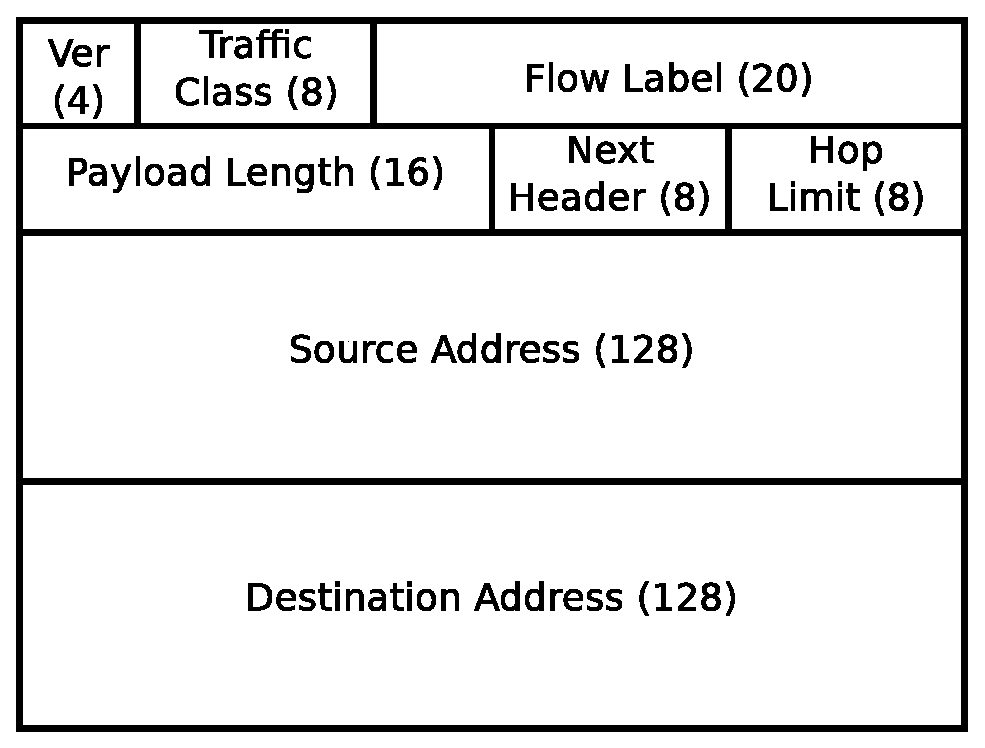
\includegraphics[width=4in]{IPv6_header}
\caption{L'en-tête IPv6}
\label{fig:IPv6}
\end{figure}

\begin{table}[htb]
\caption{Plages de valeurs pour le champ \texttt{DSCP}}
\centering
\begin{tabular}{|c|c|l|}
\hline\rowcolor[gray]{0.8}\color{black}
Plage & Valeurs & Règle d'assignation\\\hline
1 & xxxxx0 & Assignation par une norme de l'IANA\\\hline
2 & xxxx11 & Expérimentation/Usage local\\\hline
3 & xxxx01 & Expérimentation/Usage local (pourrait être jointe à la plage 1)\\\hline
\end{tabular}
\label{tab:RangesDSCP}
\end{table}

% On veut éviter que la figure et le tableau soient placés au-delà de la section courante.
% To prevent the figure and table from being positioned outside of the current section. 
\FloatBarrier


%%
%% OBJECTIFS DE RECHERCHE / RESEARCH OBJECTIVES
%%
\section{Objectifs de recherche}  % 0.5 page
Les objectifs de la recherche sont de concevoir un algorithme $O(n)$.


%%
%% PLAN DU MEMOIRE / THESIS OUTLINE
%%
\section{Plan du mémoire}  % 0.5 page

Voir la Figure~\ref{fig:Layers} pour plus de détails. 

\begin{figure}[htb]
\centering
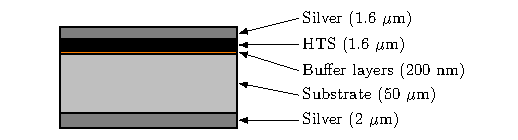
\includegraphics[width=4in]{demo_tikz}
\caption{Couches}
\label{fig:Layers}
\end{figure}


Un tableau : / A table:
\begin{table}[htb]
  \centering
  \caption{Constantes et variables du modèle analytique}
  \begin{tabular}{|c|l|}
    \hline\rowcolor[gray]{0.8}\color{black}
    Symbole         & Description\\\hline
    $\lambda$       & Taux d'arrivée moyen des requêtes de réservation de ressources\\\hline
    $\frac{1}{\mu}$ & Durée moyenne d'une session\\\hline
    $C$             & Capacité d'une cellule (nombre de sessions supportées)\\\hline
    $v_{moy}$       & Vitesse moyenne des MN dans le réseau d'accès\\\hline
    $L$             & Longueur d'un côté d'une cellule carrée\\\hline
    $n$             & Nombre moyen de MN dans une cellule\\\hline
    $\rho$          & Charge d'une cellule\\\hline
    $P_b$           & Probabilité de blocage d'une requête de réservation\\\hline
    $P_f$           & Probabilité d'interruption forcée d'une session\\\hline
    $P_c$           & Probabilité de compléter une session avec succès\\\hline
    $\Delta{}T$     & Délai de transmission\\\hline
  \end{tabular}
  \label{tab:Definitions}
\end{table}

La formule d'\mbox{Erlang-B}:
\begin{equation}
  P_b = \frac{\frac{\rho^C}{C!}}{\sum\limits_{x=0}^{C}\frac{\rho^x}{x!}}
  \label{eq:Pblock}
\end{equation}

Une autre équation : / Another equation:
\begin{equation}
  \begin{split}
    P_c &= (1 - P_b) \times (1 -  P_f)^N\\
        &= (1 - P_b)^{N+1}
  \end{split}
  \label{eq:ProbComplete}
\end{equation}

Enfin, l'expression suivante indique le moment à partir duquel les
réservations de ressources sont en place:
\begin{equation}
  \Delta{}T_{init} =
  \begin{cases}
    2\Delta{}T_{E2E} & \Delta{}T_{wan} > (\Delta{}T_{rad} + \Delta{}T_{net})\\
    \Delta{}T_{E2E} + 3(\Delta{}T_{rad} + \Delta{}T_{net}) & \text{sinon}
  \end{cases}
  \label{eq:InitCost}
\end{equation}

\paragraph{Le taux de paquets perdus} correspond au nombre de paquets
éliminés à cause d'une erreur de \emph{checksum} à un n\oe{}ud
quelconque ou d'une situation de congestion. Le taux de paquets perdus
pour un chemin est déterminé de la façon suivante:
\begin{equation}
  \label{eq:genPLR}
  PLR_P = 1 - \prod_{i=1}^N(1 - PLR_i)
\end{equation}

Toutefois, si les taux d'erreurs sont très faibles, comme c'est
généralement le cas pour des liens optiques, on peut approximer
$PLR_P$ de façon à le transformer en un paramètre additif:
\begin{equation}
  \label{eq:approxPLR}
  \begin{split}
    PLR_{L_1 \oplus L_2} &= 1 - (1 - PLR_1)(1 - PLR_2)\\
    &= 1 - (1 - PLR_2 - PLR_1 + \underbrace{PLR_1
      \times PLR_2}_\text{négligeable})\qquad PLR_1 \ll 1,
    PLR_2 \ll 1\\
    &\approx PLR_1 + PLR_2
  \end{split}
\end{equation}

\clearpage

Une courbe : / A curve:
\begin{figure}[htb]
\centering
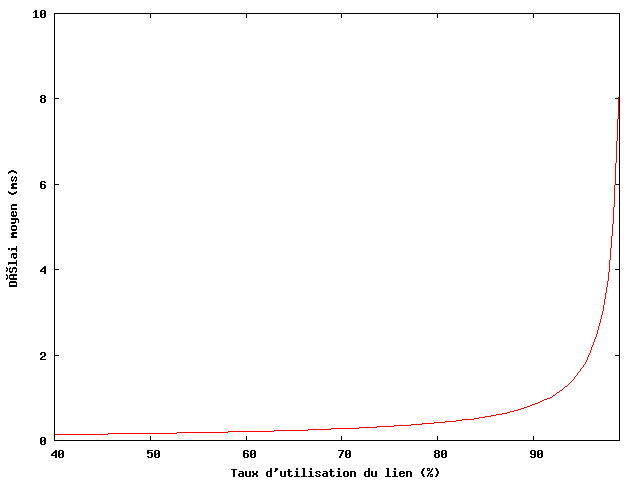
\includegraphics[width=5in]{LinkUsage}
\caption{Délai moyen en fonction du taux d'utilisation d'un lien}
\label{fig:LinkUse}
\end{figure}

\selectlanguage{english}
This paragraph is formatted by \LaTeX{} according to the standard rules of the
English language (\mbox{e.g.} hyphenation).
\selectlanguage{french}

L'arithmétique en virgule flottante peut entraîner des erreurs
d'approximation et il est important d'en être conscient
\cite{Rossi2011}.

De même, les calculs effectués sur une carte graphique (GPU) peuvent
introduire des erreurs d'approximation \cite{DeSantis2002, Cohen2006,
  Thorsson2014, Schirmer2012, Sakai2015, Electrical2006,
  Min2016, Massicotte2013, Kaliouby1987, Daintith2010, Haist2014, Kizza2013,
  Manasreh2011, Brydson1999, Boyce2002}.
       % Introduction au sujet de recherche.
\Chapter{REVUE DE LITTÉRATURE}\label{sec:RevLitt}
% Texte / Text.

\section{Robot logiciel développeur}

La définition de robot logiciel est «Agent intelligent programmé afin d'imiter les capacités d'un être humain dans un système informatique ou afin d'effectuer un ensemble de tâches prédéterminées de manière automatique.»~\cite{robot_logiciel_oqlf_2018} Les autres termes suggérés est «robot informatique» et «robot». Ainsi, un robot développeur, est un robot logiciel orienté au développement logiciel. En anglais, il pourrait être nommé un «DevBot».

La référence à l'aspect social d'un robot logiciel développeur est par exemple l'outillage aux développeurs autour d'un éditeur asynchrone en temps réel tel que CodeBuddy~\cite{10.1145/3287324.3293750} ou CodePilot~\cite{10.5555/1030453.1030540} dans leur développement collaboratif.

Le robot logiciel développeur idéal est «un développeur de logiciels artificiels qui est autonome, adaptable et possède des compétences techniques ainsi que sociales.»~\cite{8823643} Seulement les éléments des compétences techniques et sociales seront discutés dans ce mémoire, le tout orienté sur la plateforme ERPLibre avec de l'amélioration continue sur un réseau d'entraide.

\section{Génération de code}

Utiliser un générateur de code dans un contexte d'application web est efficace, l'auteur Uyanik.B, et a. de l'article «A template-based code generator for web applications»~\cite{SAHIN2020} obtient un gain de performance en temps de développement de 98.95\% et 0 bogue via le générateur de code.

Dans un autre projet de l'auteur Pichidtienthum.S et a. de l'article «»~\cite{9436754}, en ajoutant une interface LCNC sur un générateur de code sur Odoo, on obtient 20\% de réduction de temps pour le développement de module, puis des utilisateurs non développeur peuvent utiliser cet outil pour faire des modules. Ce projet est très similaire à celui expérimenté dans ce mémoire, sauf l'aspect de la rétro-ingénierie qui est manquante avec l'amélioration continue et la gestion d'un réseau d'entraide.

\section{Logiciel Libre et Open Source}

Actuellement, une méthode utilisée pour accélérer le développement, c'est le partage de bibliothèques : une fonctionnalité aurait déjà été programmé et le rendre accessible publiquement permet la réduction d’écriture du code pour réaliser une fonctionnalité souhaitée.

L’Open Source permet aussi de supporter l'interopérabilité~\cite{open_interop_2011}, c’est la capacité de différents logiciels d'interagir et communiquer efficacement entre eux de manière transparente et harmonieuse sans entraves ni obstacles, même s’ils ont été développés par différentes organisations.

D'ailleurs, comme le mentionne l'auteur Hertel.G et a. de l'article «Motivation of software developers in Open Source projects: an Internet-based survey of contributors to the Linux kernel»~\cite{HERTEL20031159}, un des facteurs de motivation important est la perception de l'indispensabilité de ses propres contributions dans une équipe, associé à une évaluation élevée des objectifs de l'équipe et un fort sentiment d'auto-efficacité personnelle. Le générateur de code ne doit pas remplacer l'utilisateur, il doit l'accompagner dans leur développement.

% \section{Logiciel Libre}
% Le logiciel libre entrave l’interopérabilité seulement pour les systèmes non compatibles avec la copyleft. Bien qu’elle prône la liberté du code, elle est restrictive.

% Cette restriction est nécessaire à la protection du développeur et de la communauté. 

\section{Sécurité}

«La morale de l'article~\cite{thompson_trusting_1984}, alors, est assez simple : il est impossible de fonctionner\footnote{D'utiliser et d'avoir confiance sur des technologies} sans faire confiance à quelqu'un. À moins que vous n'ayez écrit tout le code (et je veux dire TOUT le code) vous-même, vous devrez faire confiance à la sécurité d'une partie du processus de traitement du programme.»~\cite{discussion_reflection_trusting_2020} L'automate codeur doit apprendre à développer toute les étapes de programmation sur une machine.

Hors, s'il est nécessaire de faire confiance, peut-on faire confiance lorsqu'on observe des problème de compatibilité de licence libre~\cite{pfeiffer2022license}\cite{8667977}? Le développeur utilise des bibliothèques libres qui utilisent d'autre bibliothèques pas nécessairement libres et qui peuvent contenir des failles de sécurités~\cite{10.1145/3133956.3134048}, sans en être conscient. Le robot codeur doit ainsi être en mesure de faire du développement sur les bibliothèques utilisés.

«Cela suggère que tant que nous ne sommes pas en mesure de rétroconception\footnote{Faire de la rétro-ingénierie sur un développement.} et de contrôler pleinement la fonctionnalité des réseaux neuronaux, il existera un risque inhérent. Même si nous parvenons à résoudre le problème d'alignement et à rendre l'IA conviviale pour l'homme, les attaquants qui obtiennent un accès en écriture aux poids\footnote{Un poids est la valeur numérique d'une neurone dans un réseau de neurones.} pourront implanter leurs portes dérobées.»~\cite{discussion_reflection_trusting_ia_2023} L'automate doit être en mesure de comprendre le fonctionnement du logiciel pour l'étudier.

\section{Les complexités de développer ERP}
% TODO voir article erp en entreprise
% REF implantation d’un ERP en PME

Le développement d’une solution ERP doit supporter plusieurs niveaux~\cite{uqam_erp_benefice_2008} : 
\begin{enumerate}
    \item Évaluation des besoins;
    \item Préparation du projet;
    \begin{enumerate}
        \item Organisation du projet;
        \item Définir les objectifs;
        \item Créer un plan détaillé;
    \end{enumerate}
    \item Dessin d’affaires;
    \begin{enumerate}
        \item Analyser les processus d’affaires actuels;
        \item Maîtrise du système ERP;
        \item Revue des processus;
    \end{enumerate}
    \item Réalisation;
    \begin{enumerate}
        \item Développement technique;
        \item Étude pilote;
    \end{enumerate}
    \item Préparation finale;
    \begin{enumerate}
        \item Réglages et tests;
        \item Éduquer et former la masse critique;
    \end{enumerate}
    \item Mise en production et support;
    \begin{enumerate}
        \item Déploiement des modules ERP;
        \item Améliorer et élargir les systèmes ERP de façon continue;
    \end{enumerate}
\end{enumerate}

Autour de ça, il faut mettre en place une gestion du changement et adapter le développement des affaires.

Plusieurs de ces étapes ne sont pas prises au sérieux, tel que le financement. De plus, l’implantation se fait sur une longue période de temps.

Dans Odoo, le nombre de modules augmente avec le temps et diffère entre les versions, une recherche fastidieuse doit être effectuée pour réduire le temps de développement et à éviter de réinventer la roue.

Il faut adapter les processus des organisations aux fonctionnalités existantes, sinon il est trop coûteux de tout recréer selon les processus de l’entreprise.

En plus de suivre toutes ces étapes, il faut mettre en place une pérennité pour l’amélioration continue sur le projet, cela rend le processus lourd en plus de durer dans le temps.


\section{Logiciel no-code / low-code}

Logiciel no-code / low-code = LCNC

Basé sur des templates de code et une interface qui, au besoin, permet la configuration par du code.

C’est un concept qui permet à l’utilisateur de développer une plateforme en utilisant pas ou peu de code.

% TODO REF A. C. Bock, U. Frank: Low-Code Platform, Bus Inf Syst Eng 63(6):733–740 (2021)
% TODO REF Supporting the understanding and comparison of low-code development platforms

Besoin de : 
\begin{enumerate}
    \item Aspect général;
    \begin{enumerate}
        \item Gestion des rôles et permissions par des groupes utilisateurs ou individuelle;
        \item Mécanisme de déploiement et exportation;
    \end{enumerate}
    \item Perspective d’intéraction;
    \begin{enumerate}
        \item Mécanisme pour changer le design de l’interface utilisateur;
        \item Mécanisme pour coupler l’interface à un modèle et un contrôleur (MVC);
        \item Mécanisme pour faire le rendu visuel sur différents types d’appareils;
    \end{enumerate}
    \item Perspective dynamique;
    \begin{enumerate}
        \item Gestion des processus du système et de la machine;
        \item Composantes de modélisation de processus conceptuel;
        \item Système de gestion des états et des transitions;
    \end{enumerate}
    \item Perspective fonctionnelle;
    \begin{enumerate}
        \item Mécanisme de spécification fonctionnel de base;
        \item Générateur d’algorithme;
        \item Générateur de code de composantes;
        \item Mécanisme d’accès à des API externe;
    \end{enumerate}
    \item Perspective statique;
    \begin{enumerate}
        \item Composante de conception d’un modèle de données;
        \item Composante pour spécifier des structures de données;
        \item Gestion de base de données interne;
        \item Gestion de base de données externes par API;
    \end{enumerate}
\end{enumerate}

Pour supporter une plateforme LCNC :
\begin{enumerate}
    \item Bases de données;
    \item Services externes;
    \item Gestion des modèles de données;
    \item Plateforme collaborative;
    \item Service infonuage (déploiement, audit de performance, gestion des erreurs/traces/événements, gestion des versions);
    \item Générateur de code;
    \item Compilateur et optimiseur de code;
    \item Modeleur d’application;
    \begin{enumerate}
        \item Widget;
        \item Connecteur;
        \item Processus de logique métier;
        \item Capacité de «drag and drop»;
        \item Modèle de données;
        \item Règles de sécurité;
    \end{enumerate}
\end{enumerate}
Critère de qualité d’une plateforme LCNC :
\begin{enumerate}
    \item GUI;
    \item Interoperability support entre services externes et base de données;
    \item Support de la sécurité;
    \item Support d’une plateforme collaborative;
    \item Support sur la réusabilité, pouvoir répété l’utilisation d’une composante dans différents contextes;
    \item Support de la capacité d’un système à maintenir ou à améliorer ses performances;
    \item Mécanisme de spécification de logique du développement des affaires;
    \item Logiciel pour construire des mécanismes;
    \item Support au déploiement;
\end{enumerate}

% \section{Dev ops}
% Démontrer outil
% TODO image dev ops

% La partie générateur de code répond seulement au besoin création de code du dev ops.

\section{Création d’une communauté}

\subsection{Communication non violente}

Réduire les frictions entre les participants du réseau d’entraide. C’est avec la mise en place d’une méthode de communication non violente~\footnote{\url{https://fr.wikipedia.org/wiki/Communication_non_violente}} formalisée par Marshall B. Rosenberg, voir Figure~\ref{fig:communication_non_violente}.

\begin{figure}[htb]
\centering
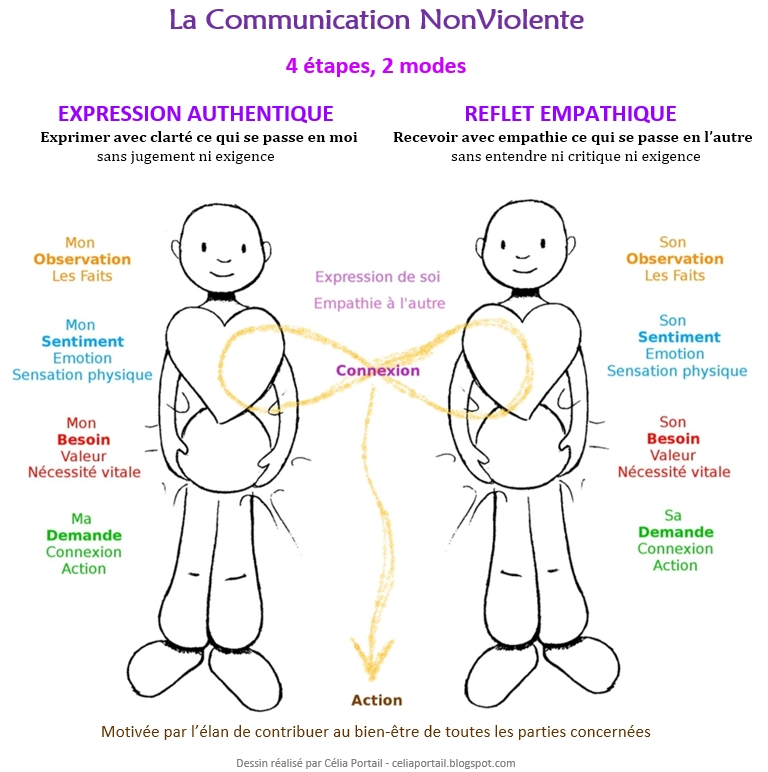
\includegraphics[width=4in]{OSBD_en_CNV.jpg}
\caption{Communication non violente en 4 étapes et 2 modes}
\label{fig:communication_non_violente}
\end{figure}

\subsection{Guide construire une communauté Open Source}
Guide en 4 sections avec des titres indicateurs d’orientation pour un gestionnaire de communauté :

\begin{enumerate}
    \item Mise en place de votre projet pour le succès;
    \item Cultiver votre communauté;
    \item Résoudre les conflits;
    % \item La communauté est le coeur ❤️ de l’open source.
    % \item La communauté est le coeur ❤ de l’open source.
    \item La communauté est le coeur de l’open source.
\end{enumerate}

Il faut :
\begin{enumerate}
    \item rédiger un code de conduite;
    \item proposer la contribution directement sur le projet.
\end{enumerate}
% TODO supporter les autres pages https://opensource.guide/fr/metrics/

Ils n'intègrent ni les aspects de génie industriel qui est vulgarisé avec le guide fusée et ni les critères éthiques de GNU concernant l’hébergement de logiciel.

\subsection{Guide fusée}

Un guide en 7 étapes~\ref{fig:guide_fusee} pour les gestionnaires de projet. Il vous permet de démarrer un projet rapidement qui nécessite une équipe de personnes pour les rendre efficaces dans la réalisation de leurs participations dans le réseau d’entraide.

% REF guide fusée polylabac/cimarlab

\begin{figure}[htb]
\centering
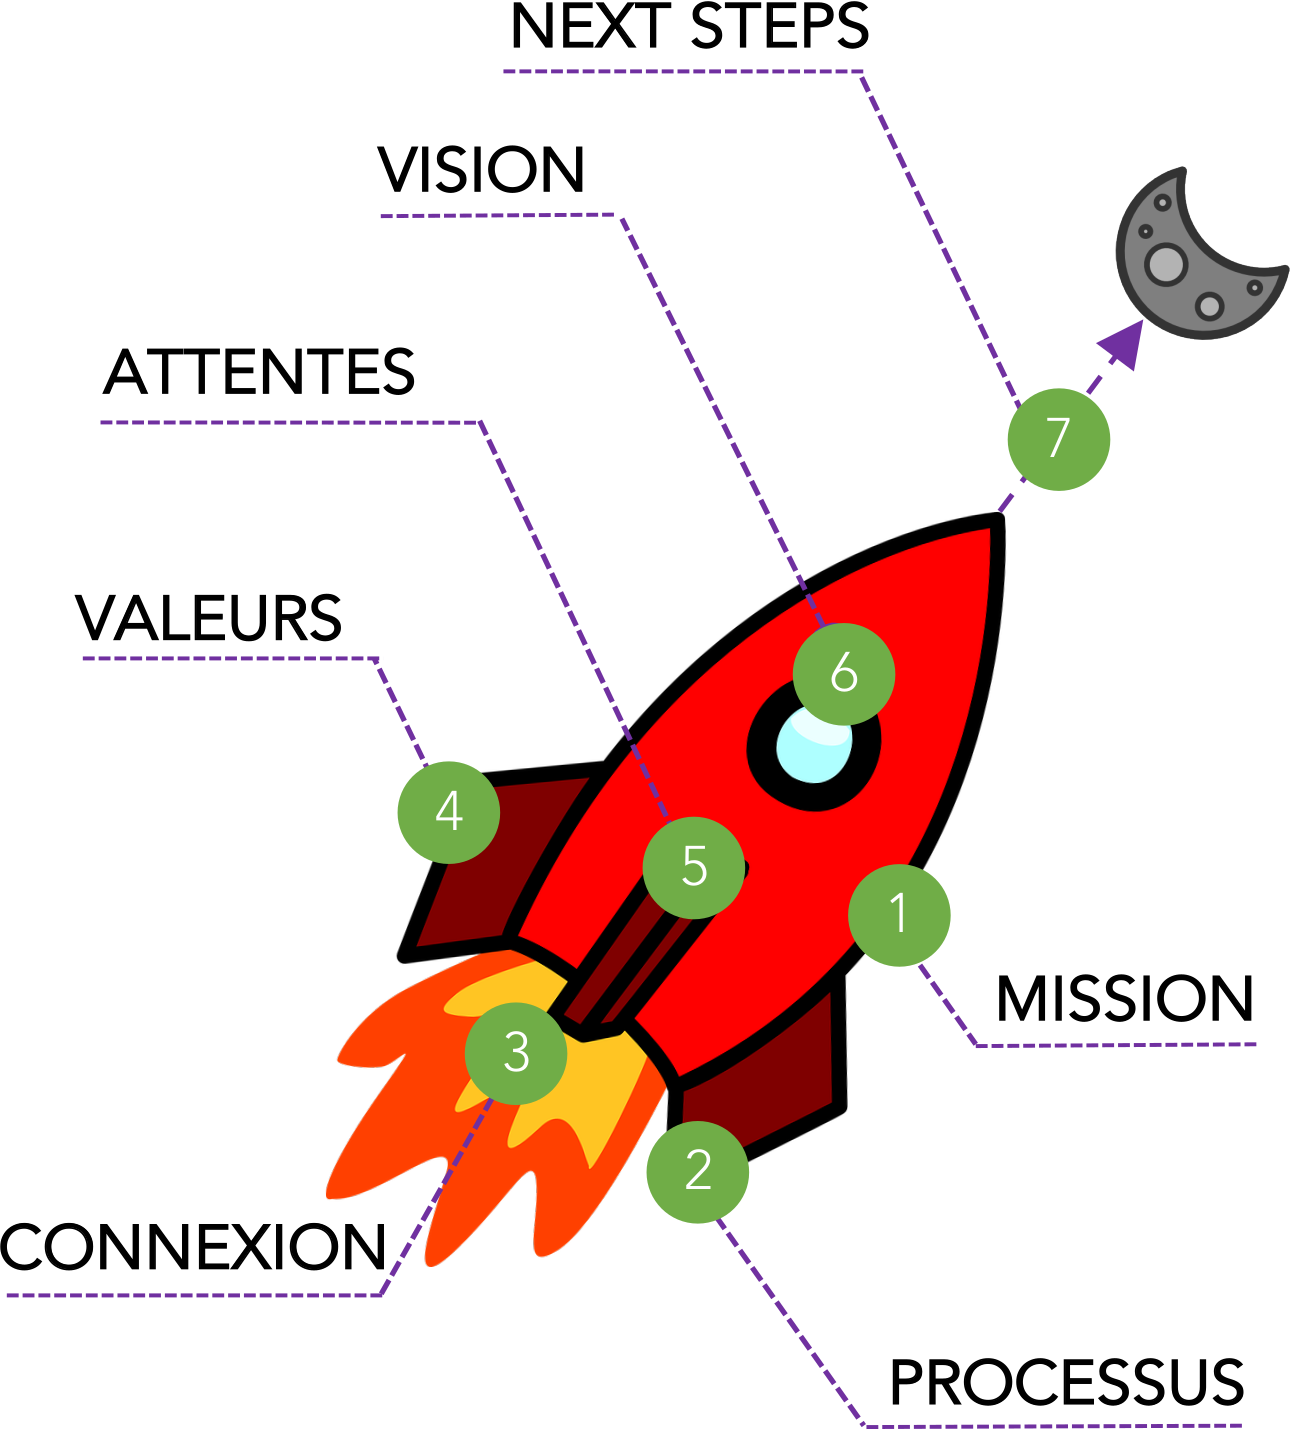
\includegraphics[width=4in]{guide_fusee_definition.png}
\caption{Guide fusée de CimarLab}
\label{fig:guide_fusee}
\end{figure}

\subsection{Critères éthiques de GNU concernant l'hébergement de logiciel}

La licence AGPLv3 n’est pas toujours bien respectée~\cite{violation_libre_2017}.

Les critères éthiques concernant l'hébergement de logiciel~\cite{gnu_critere_hebergement_2022} doivent être accessibles sur les projets de réseau d’entraide. Un guide avec des critères mesurables pour les services destinées à tous ceux qui veulent utiliser un service pour héberger publiquement du code source libre, ainsi qu'éventuellement des programmes exécutables. Ces critères se concentrent sur la protection de la vie privée, le fonctionnement sans JavaScript non libre\footnote{\url{https://www.fsf.org/campaigns/freejs}} , la compatibilité avec les licences à copyleft et leur philosophie, et l'absence de discrimination contre les utilisateurs, quels qu'ils soient.  Les questions à répondre : 

\begin{enumerate}
    \item Est-ce que l'hébergeur fournit l'accès au code source des programmes qu'il héberge?
    \item Est-ce que l'hébergeur permet la redistribution des copies des programmes qu'il héberge?
    \item Est-ce que l'hébergeur permet aux utilisateurs d'apporter des modifications aux programmes qu'il héberge et de les partager avec la communauté?
    \item Est-ce que l'hébergeur impose des restrictions sur l'utilisation ou la redistribution des programmes qu'il héberge?
    \item Est-ce que l'hébergeur respecte les licences de logiciels libres et les droits d'auteur associés aux programmes qu'il héberge?
    \item Est-ce que l'hébergeur fournit des informations sur les licences de logiciels libres et les droits d'auteur associés aux programmes qu'il héberge?
    \item Est-ce que l'hébergeur respecte la vie privée et la sécurité des utilisateurs des programmes qu'il héberge?
    \item Est-ce que l'hébergeur fournit un support et une assistance adéquats aux utilisateurs des programmes qu'il héberge?
\end{enumerate}

\section{Poïèse}

\subsection{Définition de la poïèse}

La poïèse (ou poïesis) est un terme d'origine grecque qui désigne le processus créatif de fabrication, de production ou de création. Il est souvent utilisé dans le contexte de l'art et de la littérature pour décrire le processus de création d'une œuvre, que ce soit un poème, une pièce de théâtre, un roman ou une peinture.

Dans ce contexte, la poïèse est considérée comme un processus actif et dynamique, impliquant l'imagination, l'inspiration, la créativité et la maîtrise technique. Elle implique souvent un certain niveau d'engagement personnel et émotionnel de la part de l'artiste\label{poiese_artise} ou du créateur.

En dehors de l'art, le terme poïèse peut également être utilisé pour décrire tout processus de création ou de production, y compris dans des domaines tels que la science, la technologie ou l'industrie.

Les termes «Allopoïèse», «Autopoïèse», «Sympoïèse» ont été inventés pour décrire des phénomènes biologiques, hors dans ce mémoire, ils ont été adaptés pour un contexte technologique.

\subsection{Allopoïèse}

Un système qui développe\footnote{production/fabrication : Utiliser sans limitation, Modifier pour adapter, Étudier pour comprendre le fonctionnement et Copier pour reproduire.} quelques choses avec des composantes externes.

«L'allopoïèse est le processus par lequel un système produit quelque chose qui n'est pas le système lui-même. Ceci est le contraire de l'autopoïèse.[...] La plupart des processus de production industrielle sont allopoïétiques : une chaîne de montage peut produire des voitures mais pas les machines utilisées dans cette forme de production. [...] La reproduction n'est pas une auto-production.»~\cite{wiki_allopoiesis_2018}~\cite{vuc_allopoiesis_2018}


% «une définition qui est proche de celle d’une machine abstraite et qui décrit la machine comme autopoïétique, autoproductrice d’elle-même et reproduisant en permanence ses composantes tel un système sans input ni output. Varella développe assez loin cette théorie. Il oppose dans sa conception, l’autopoïèse qu’il rapporte essentiellement aux êtres vivants biologiques, à une allopoïèse où la machine va chercher ses composantes à l’extérieur d’elle-même. En fait, dans son concept d’allopoïèse il range les systèmes sociaux, les machines techniques et, pour finir, tous les systèmes machiniques qui ne sont pas des systèmes vivants.»
% «Les machines allopoïétiques se trouvent toujours en adjacence à des machines autopoïétiques et il faut donc prendre en considération les agencements qui les font vivre ensemble.»
% Citer ce document / Cite this document :
% Guattari Félix. À propos des machines. In: Chimères. Revue des schizoanalyses, N°19, printemps 1993. pp. 85-96 ;
% doi : https://doi.org/10.3406/chime.1993.1881
% https://www.persee.fr/doc/chime_0986-6035_1993_num_19_1_1881


\subsection{Autopoïèse}

Un système qui se développe par soi même avec seulement ses composantes internes.

«L'autopoïèse est la propriété d'un système de se produire lui-même, en permanence et en interaction avec son environnement, et ainsi de maintenir son organisation (structure) malgré son changement de composants (matériaux) et d'informations (données).[...]le maintien de sa propre organisation (auto-production)»~\cite{wiki_autopoiesis_2022}.

Le maintien de sa propre organisation signifie l'auto-production, voir exemple illustratif auto-reproducteur~\ref{exemple_illustratif_auto_reproducteur}.

Un système est de l'autopoïèse~\cite{tatsuya_computational_autopoiesis_2000} dans le contexte qu'il est : 
\begin{enumerate}
    \item \textbf{Autonome} : il doit être capable d'apporter des changements variés pour maintenir son organisation;
    \item \textbf{Individuel} : il doit être indépendant dans sa définition, par sa prise de décision par rapport aux observateurs externes, en reproduisant à répétition et en maintenant son organisation;
    \item \textbf{Connaissant et établis ses limites} : il doit être capable d'établir ses limites dans son processus de reproduction par lui même sans se faire affecter des limites établis par les observateurs externes;
    \item \textbf{Absent d'entrant et de sortant} : Les stimulis externes doivent être interprété dans un contexte d'observation pour en retirer de l'amélioration continue, elles ne doivent pas impacter la maintenance de l'organisation directement, mais son évolution doit en prendre compte.
\end{enumerate}

Le concept de vue sur les entrants et sortants d'un système est une perception des observateurs externes et ne clarifie pas l'organisation ou les opérations de production du système. 

% TODO à valider : Ainsi, le système va opérer sans s'ajuster lui-même en rapport avec son état et le stimulis externe.

% TODO Alors comment fait-il pour se produire lui même en interaction avec son environnement s'il n'a pas d'entrant et sortant?

La conception d'un système autopoïèse\cite{tatsuya_computational_autopoiesis_2000} devrait comporter les points suivants : 

\begin{enumerate}
    \item Les composantes du système sont déterminés par les opérations du système;
    \item Les opérations du système sont produites avant les conditions initiales;
    \item Les opérations du système sont seulement exécutées pour leur propre réussite et non pour réaliser la production d'un produit;
    \item Dans les opérations du système, ce qui se passe à l'intérieur du système est clairement différent des jugements des observateurs externes.
\end{enumerate}

% TODO La Technopoïèse doit être différent de l'autopoïèse, bien qu'il doit être autonome dans son évolution, il doit suivre des principes moraux et respecter des règles de société.

%  L'autopoïèse s'applique aussi à l'être humain, tant en sociologie\footnote{\url{https://fr.wikipedia.org/wiki/Sociologie}}, la science cognitive\footnote{\url{https://fr.wikipedia.org/wiki/Sciences_cognitives}}, la philosophie\footnote{\url{https://fr.wikipedia.org/wiki/Philosophie}} et la psychopathologie\footnote{\url{https://fr.wikipedia.org/wiki/Psychopathologie}}.

Appliquer l'autopoïèse sur un système est de forcer un changement de point de vue vers l'intérieur du système, puisque l'extérieur est matière à interprétation par la distinction de son environnement. En sciences naturelles, ce changement de point de vue est difficilement acceptable puisque le point de vue est fait par des observateurs externes.

Des modèles mathématiques sont expliqués dans l'article~\cite{tatsuya_computational_autopoiesis_2000} tel un système de réparation du métabolisme ((M,R) systems), introduit par Rosen, pour démontrer le «Quasi-Autopoietic Systems».
Puis il y a des modèles d'apprentissage automatique qui ont été inspirés de l'autopoïèse pour effectuer des tâches de reconnaissance de formes. Pour pouvoir représenter l'autopoïèse en mathématique ou en modèle informatique, il est nécessaire de trouver un mécanisme d'un système qui crée son espace avec ses limites et son environnement, par soi-même.

% TODO documentation intéressante : https://www.researchgate.net/publication/228784157_A_Computational_Aspect_of_Autopoiesis

\subsection{Sympoïèse}

Un système qui développe en collectivité. Caractéristique d'une technologie qui fait de la poïèse.

La sympoïèse est un concept utilisée en écologie et en théorie des systèmes pour décrire les processus de production collective et collaborative dans les écosystèmes. Elle se distingue de l'autopoïèse, qui est le processus par lequel un système produit et reproduit ses propres composants de manière autonome. Par exemple, les coraux sont des collectifs d'organismes en interaction qui produisent des structures complexes telles que des récifs, qui ont des effets bénéfiques sur l'écosystème dans son ensemble.

«La nature est une puissance d’engendrement qui surgit et s’autoproduit. Donna Haraway a récemment proposé de remplacer le concept "d’autoproduction" par celui de "sympoïèse" qui désigne la coproduction du milieu par des espèces en interrelations plutôt que l’activité autonome de certains organismes isolés.»~\cite{guillibert:tel-02929676}

\subsection{Technopoïèse}

Un système technologique qui développe. Caractéristique d'une technologie qui fait de la poïèse.

% Un système technologique qui travaille pour la poïèse en mettant en place plusieurs caractéristiques, par exemple : l'«Allo» et l'«Auto».

La technologie est là pour assister l'utilisateur et l'accompagner dans l'évolution de celle-ci. «Parce que l’appareil prend place entre la manifestation de l’œuvre et le travail de l’artiste en les découplant, en leur imposant une langue intermédiaire qui code puis décode. L’artiste produit des lignes de code, que la technologie intègre pour fournir à l’œuvre la source de sa manifestation : elle sépare ontologiquement\footnote{Une ontologie est une représentation formelle et explicite de la connaissance d'un domaine, qui spécifie les concepts, les relations et les entités qui existent dans ce domaine et comment ils sont interconnectés.} le travail de l’un et son résultat dans l’autre.»~\cite{artiste_techno_conf_2012} L'artiste~\footnote{Voir l'artiste de la «Définition de la poïèse»~\ref{poiese_artise}} ici signifie un programmeur informatique dans un processus créatif de fabrication, de production ou de création sur des technologies.

Pour éviter que la machine prend le dessus, il faut l'orienter vers la technopoïèse. «Si la technologie est un médium parasite, alors ne suffit-il pas de compter sur la charge poïétique du médium primaire, pour conserver à la poïèse ses caractères nécessaires – et imaginer l’art technologique comme un art d’abord, agrémenté, partiellement seulement, de technologie?»~\cite{artiste_techno_conf_2012} % Cette machine doit être libre pour respecter l'humain. % TODO référence machine libre respect humain

%«Our main claim in this study is to underline that the biopoetic process organizing technopoiesis involves at least four levels, with emergences and constrains between the levels. Furthermore, we see technopoiesis as the dynamics between these four levels based on mechanisms expressing the relation between biology, poetics and external representations that cognitively and socio-culturally ground the evolution of technology.»~\cite{10553_41343}

La relation entre la sympoïèse et la technopoïèse permettrait de concevoir des technologies plus durables et écologiquement responsables, qui favorisent la production collective et collaborative dans les écosystèmes.

Ainsi, le terme «technopoïèse» fait référence à la capacité de l'humanité à créer et à façonner la technologie pour répondre à ses besoins et à ses désirs. 

\subsection{Auto-technopoïèse}

% TODO source chatgpt

% L'auto-technopoïèse étend cette idée, de la technopoïèse, en suggérant que les systèmes technologiques peuvent devenir autonomes et se réguler eux-mêmes sans l'intervention humaine.

L'auto-technopoïèse est un concept qui décrit la capacité des systèmes technologiques à s'auto-organiser et à s'auto-réguler. Plus précisément, l'auto-technopoïèse se réfère à la capacité des systèmes technologiques à maintenir leur propre structure, leur fonctionnement et leur évolution, en utilisant des mécanismes internes de régulation et d'adaptation.

% Le terme "technopoïèse" fait référence à la capacité de l'humanité à créer et à façonner la technologie pour répondre à ses besoins et à ses désirs. L'auto-technopoïèse étend cette idée en suggérant que les systèmes technologiques peuvent devenir autonomes et se réguler eux-mêmes sans l'intervention humaine.

% Un exemple d'auto-technopoïèse est l'Internet, qui est un système complexe de réseaux informatiques interconnectés à l'échelle mondiale. L'Internet est capable de s'auto-réguler et de s'adapter à des changements dans son environnement, tels que l'augmentation du trafic de données ou les pannes de serveurs. Cela est rendu possible grâce à des mécanismes internes de régulation, tels que les protocoles de communication standardisés et les systèmes de routage dynamique.

% En résumé, l'auto-technopoïèse est un concept qui décrit la capacité des systèmes technologiques à s'auto-organiser et à s'auto-réguler. Cette capacité est de plus en plus importante à mesure que les systèmes technologiques deviennent plus complexes et interconnectés.

Pour faire des améliorations technologiques dans la société, sur des réseaux d'entraide, il faut orienter l'auto-technopoïèse dans de la R\&D~\cite{innovation_complex_social_system_2010} orienté aux besoins technologiques dans la gestion de cas d'urgence humanitaire, par exemple le «mouvement des villes en transition»~\cite{MOUV_063_0130}\footnote{\url{https://fr.wikipedia.org/wiki/Ville_en_transition}}, en lien avec la sympoïèse.

% https://transitionlibre.ca

% Référence : 
% Teubner, G. (1993). Autopoietic law: A new approach to law and society. Walter de Gruyter.
% Luhmann, N. (1986). The autopoiesis of social systems. John Wiley & Sons.
% Castells, M. (1996). The rise of the network society. Blackwell Publishers.
% Ahrweiler, P. (2012). Innovation in complex social systems. Routledge.
  % Revue de littérature / Literature review
\Chapter{MÉTHODE}\label{sec:Theme1} \label{chapitre_methode}

L’objectif général de ce projet a été de créer et de valider le fonctionnement d’un automate générateur de code qui sert à l’implantation d’un ERP libre. Plus spécifiquement, les travaux ont été concentré sur les cinq sous-objectifs suivants:

\textbf{SO-1} développer un générateur de code de module sur Odoo,

\textbf{SO-2} développer une logique d'amélioration continue sur l'écriture du code,

\textbf{SO-3} développer une interface permettant de paramétrer la génération de code,

\textbf{SO-4} développer un système de distribution,

\textbf{SO-5} développer un système de gestion de communauté.

La méthodologie Agile a été adopté pour le développement de ces composantes d'un automate générateur de code. Les fonctionnalités de génération de code ont été validées par des tests de comparaison entre les codes générés et les codes révisés par le développeur.

% TODO mettre à jour avec les nouveaux résultats
% TODO mettre au passé
% TODO mettre en texte les étapes en dessous

\section{SO-1 - Générateur}
Développer une logique d’écriture de module sur une architecture de MVC avec support de plateforme web. Mise en place d’un concept de gabarit de code qui génère du code. Mise en place de la génération de code à partir de données. Générer un module à partir d’une base de données externes.

\section{SO-2 - Rétro-ingénierie}
Développer la capacité de comprendre une structure de code et de la reproduire. Définir ce que c’est de l’amélioration continue et son application dans un contexte d’automatisation. Mise en place de test de validation de code sur des critères de qualité mesurables. Intégration de règles de codage standardisées pour favoriser le réseau d’entraide.

\section{SO-3 - Interface}
Proposer une classification des techniques que l’automate peut réaliser en programmation. Développer un interface permettant le contrôle de l’automate pour l’orienter dans la programmation de fonctionnalités. Rendre disponible une interface LCNC pour permettre aux utilisateurs de programmer leurs fonctionnalités.

\section{SO-4 - Déploiement}
Développer un système de distribution de l’automate.

\section{SO-5 - Réseau d’entraide}
Documenter les processus de développement pour amener les utilisateurs à contribuer et les faire participer à la maintenance. Mettre des guides pour permettre le sentiment d'appartenance. Mettre en place une politique tolérance zéro avec un système de communication non violente et créer un lieu de discussion public. Élaboration du prototype pour les spécifications du réseau de l’Accorderie du Canada. Élaboration du prototype pour les spécifications de l’organisme CEPPP du Canada.

\section{Environnement informatique}
La plateforme ERPLibre 1.5.0 contenant Odoo 12 communauté, qui utilise les langages Python 3.7, XML, Javascript et SCSS. Nos tests et développement ont été effectués sur le système d’exploitation Ubuntu 20.04.
Pour les temps d’exécution des tests, ils ont été effectués sur une machine avec le CPU AMD Ryzen 9 5950X, mémoire ram 2x«32GiB DIMM DDR4 Synchronous Unbuffered (Unregistered) 2667 MHz (0.4 ns)», et disque 1To wd-black-sn850-nvme.
Toutes les commandes utilisées sont faites à partir de la racine du projet ERPLibre.

\section{Méthodologie de test}
Les tests ont été codés directement dans ERPLibre dans un script Python avec un ensemble de script pour valider les différences dans le Git après exécution, et cacher des différences.

Le tout a été programmé avec la technique parallélisme avec la bibliothèque Asyncio et des nouveaux processus et non des «thread»\footnote{Processus légé}. Seul le test de nouveau projet est exécuté après le parallélisme ajouter plus de temps à l’exécution.

Puisque le test d’un générateur de code consiste à valider ce qu’il a généré, ainsi vérifier la couverture de code est un bon indicateur pour déterminer le code utilisé et validé ce qui est déprécié dans le générateur.

\subsection{Couverture du code}
La couverture du code a été faite avec la bibliothèque «Coverage» version 7.0.1 en Python et configurée sur le répertoire qui contient le générateur de code pour faire le suivi des lignes exécuter dans la machine. Ça devient une métrique de la performance d’utilisation sur la quantité de fonctionnalité généré.
             % Premier thème (Doctorat) ou "Détails de la Solution" (Maîtrise) / First topic (PhD) or "Details of the Solution" (Master's).
\Chapter{RÉSULTAT EXPÉRIMENTAUX}\label{sec:Theme2}

Nous présentons les résultats en commençant par décrire l’implémentation du modèle conceptuel du robot logiciel codeur présenté dans la sous-section~\ref{subsection_cadre_conceptuel}. Ensuite, nous présenterons successivement les résultats propres à chacun des sous-objectifs décrits dans le chapitre~\ref{chapitre_methode}.

\section{Implémentation: du modèle conceptuel au modèle opérationnel}

L’implémentation de la machine (conceptuelle) est passée par la programmation manuelle d’une première interface et d’un premier noyau, en mettant à jour une version préliminaire de générateur, basée sur une GUI\cite{bluiksnot_repo} en lui intégrant la capacité de générer du code à partir d’un module externe via son \textit{hook} au moment de l’installation. La version à ce jour, ainsi que ses guides d’utilisation et ses scripts associés, sont disponibles sur le site de ERPLibre\footnote{\url{https://erplibre.ca}}.

L’interface permet l’interactivité avec un utilisateur ou le système-cible. Dans le cadre conceptuel~\ref{subsection_cadre_conceptuel}, l’interface est découplée en deux ensembles de méta-données: µ$_C^A$ et µ$_C^B$. µ$_C^B$ est l’ensemble qui paramétrise le passage de méta-données au code pour un module spécifique. µ$_C^A$ est l’ensemble qui paramétrise le passage de code aux méta-données, tout en préparant un µ$_C^B$ adapté à ce module spécifique. Ce découplage a permis l’adaptation de l’interface au contexte de l’installation de modules sur une instance Odoo via des \textit{hooks}. Par la suite, un ensemble supplémentaire de méta-données, noté µ$_C^0$, a été dégagé de la programmation manuelle de versions successives de µ$_C^A$. µ$_C^0$ sert à initialiser une version de départ de µ$_C^A$.

Le noyau prend les paramètres issus de l’interface pour créer des méta-données, générer l’ensemble des fichiers des modules désirés (mode direct) et faire de la rétro-ingénierie (mode indirect) sur des modules existants.

\subsection{Développement et amélioration continue}

Dans la Figure~\ref{fig:dia_sequence_gc}, µ$_C^0$, µ$_C^A$, µ$_C^B$, $C$ et $M$ sont tous des modules installables sur Odoo. $M^i$ et $M^d$ sont des sections de code dans le module $M$. µ$_C^0$, µ$_C^A$ et µ$_C^B$ dépendent de $M$. µ$_C^A$, ce sont les macro-méta-données, alors que µ$_C^B$, sont les micro-méta-données.

\begin{figure}
\centering
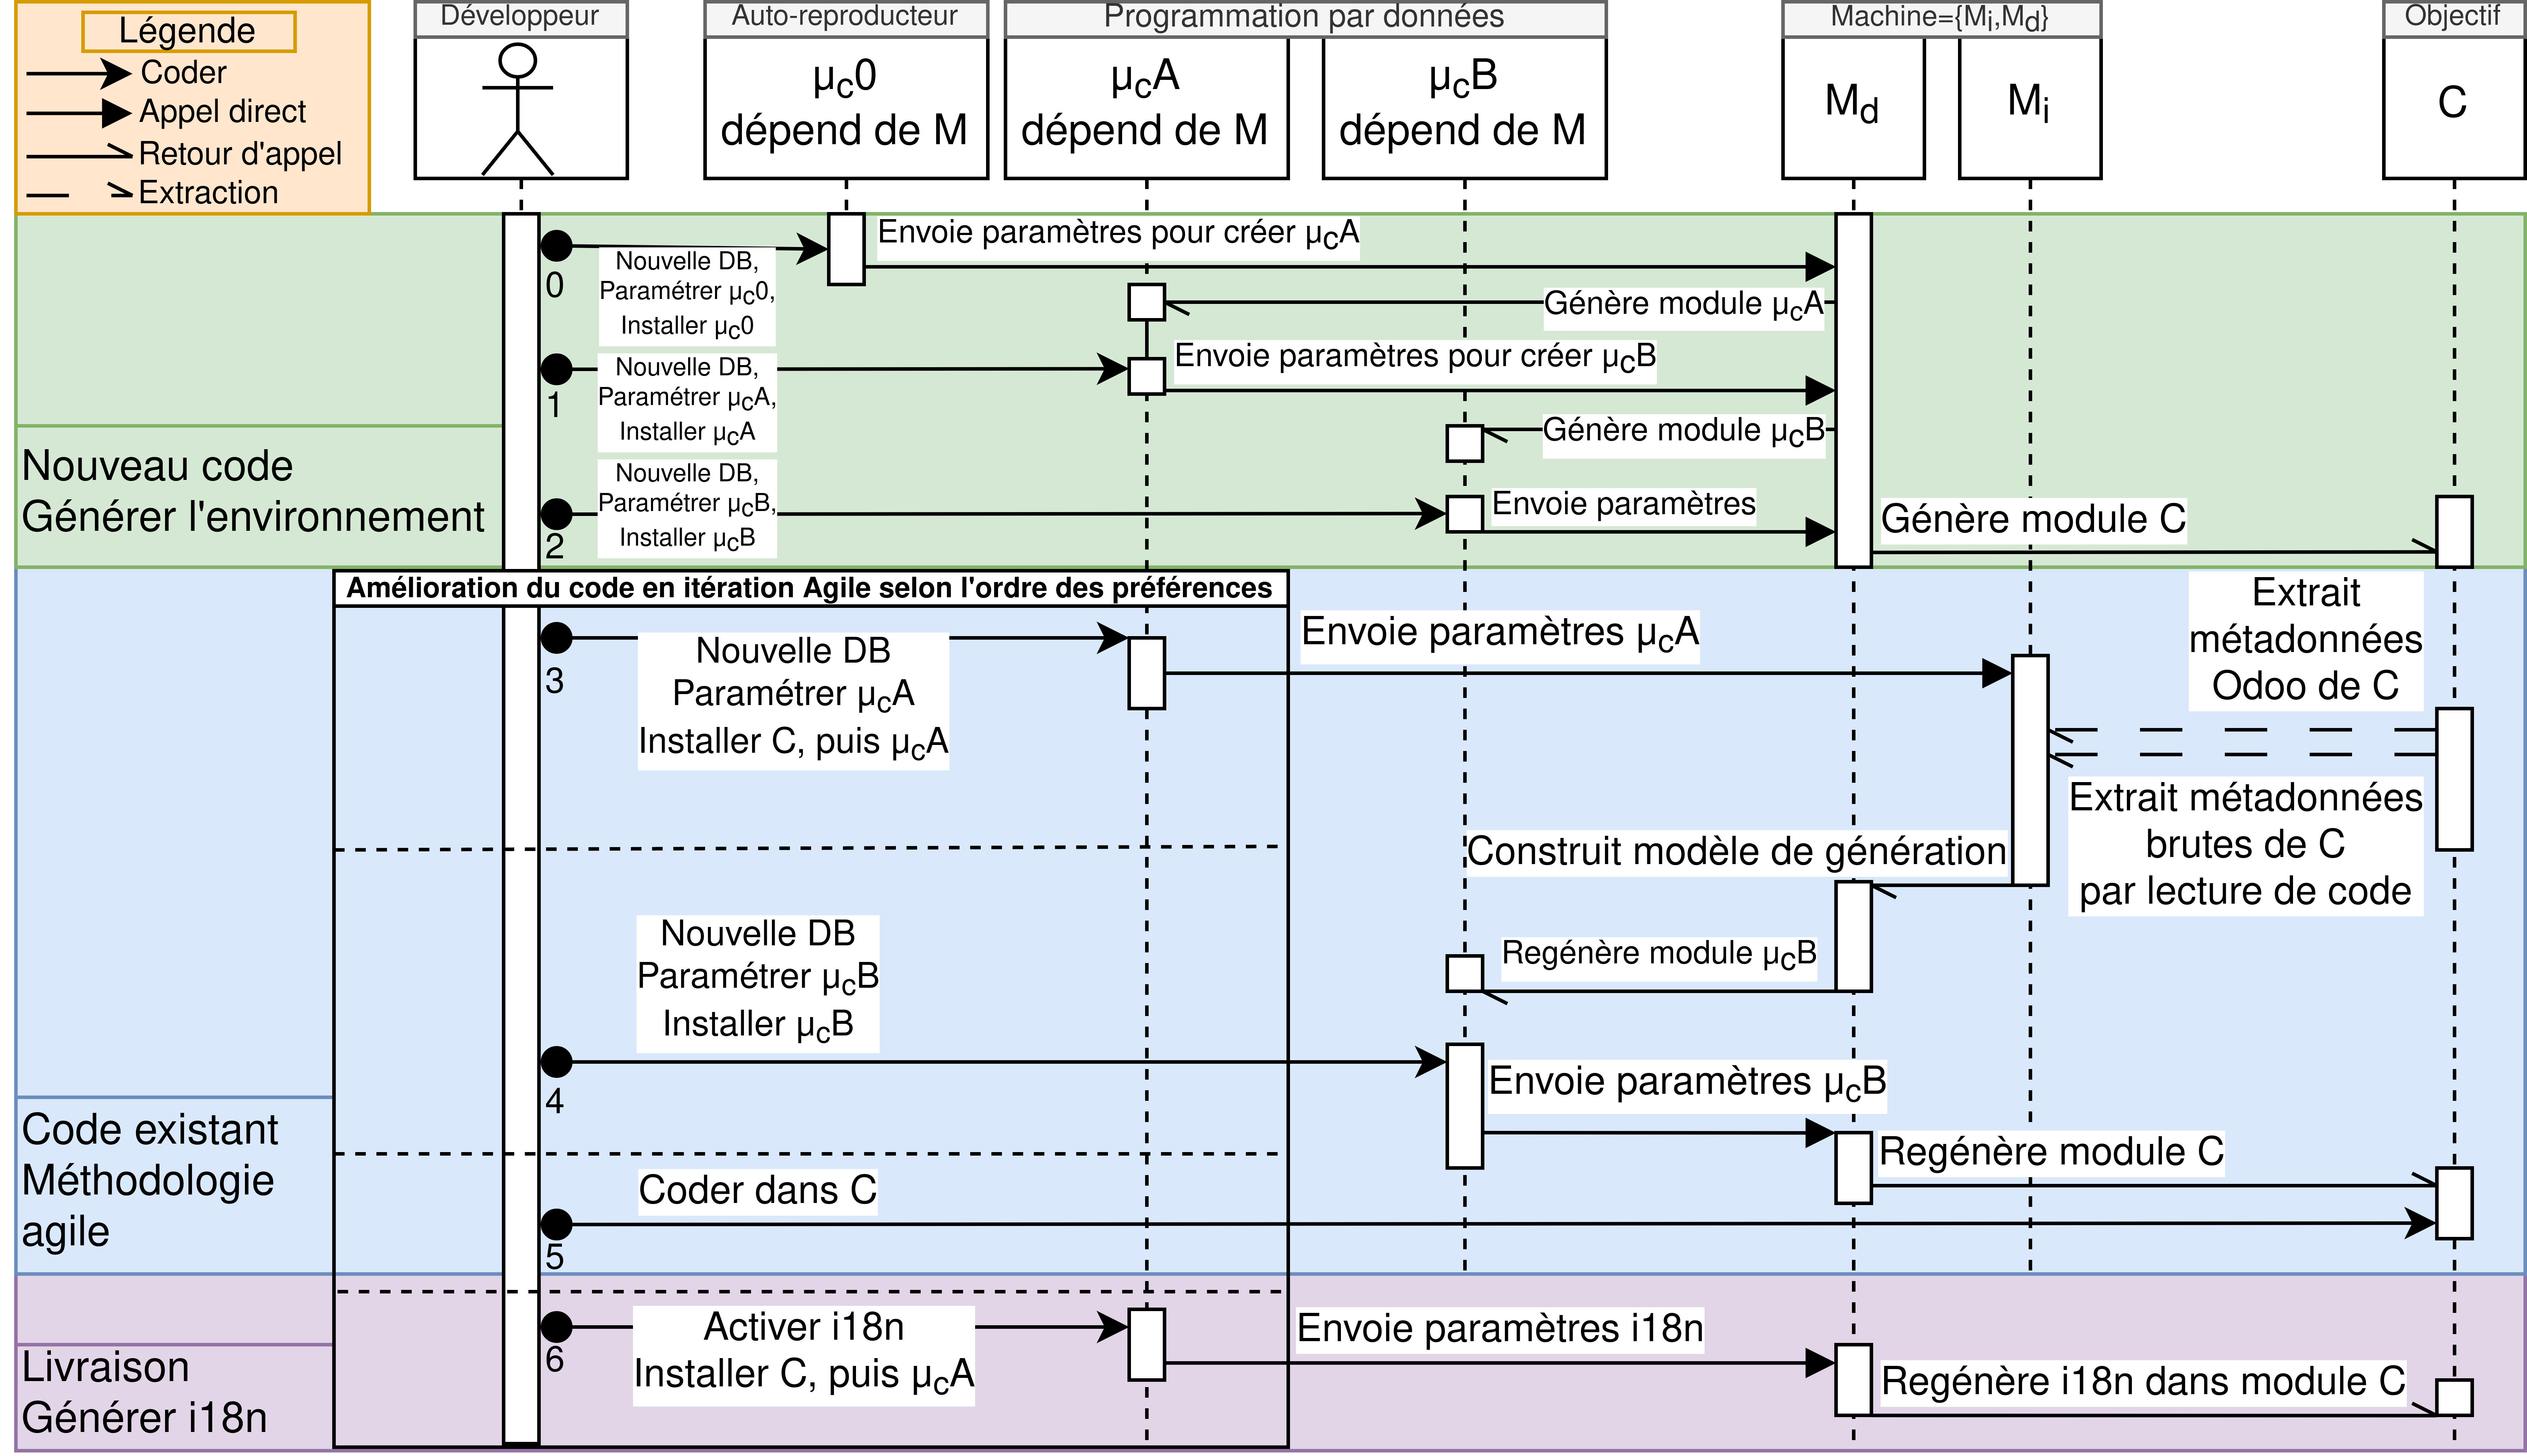
\includegraphics[width=6.535in]{images/code_generateur_erplibre_global_sequence.drawio.png}
\caption{Interaction du développeur avec le générateur de code}
\label{fig:dia_sequence_gc}
\end{figure}

Au départ d’un nouveau module code, µ$_C^0$ génère µ$_C^A$ qui génère µ$_C^B$ qui génère $C$. Il existe un script qui automatise un nouveau code, le développeur peut paramétrer le nom des modules et leurs emplacements. Ensuite, le développement commence en itérations agiles, les actions de 3 à 6 peuvent être exécutées dans l’ordre du choix du développeur.

Passer par l’étape 3 permet de mettre à jour l’étape 4, selon l’état du code, grâce à la rétro-ingénierie. L’étape 4 permet de mettre à jour le code selon le générateur. Il est possible de générer de nouvelles sections, comme la vue portail. Passer à l’étape 5 permet de personnaliser le code directement alors que l’étape 6 permet de mettre à jour le i18n de manière automatique.

La livraison sert à générer le i18n. C’est Odoo qui le génère, mais le générateur envoie les commandes, la liste des langues désirées à supporter et place les fichiers aux bons endroits dans le module. La raison pour laquelle c’est µ$_C^A$ qui doit le générer, c’est parce que le module doit être fini d’être généré et chargé de nouveau, pour ensuite générer les langues, sinon elles sont corrompus par les traces de µ$_C^B$.

% TODO mettre dans discussion : Dans un contexte où l’ingénierie et la rétro-ingénierie serait parfaite, on n’aura pas besoin de mémoriser µ$_C^A$ et µ$_C^B$. Entre-temps, il y a une intervention humaine sur chacun de ces modules pour accélérer le développement. L’outil Git est utilisé pour faire des comparaisons entre les états d’itérations, seul ce qui est commité contient le bon contenu.

\subsection{Architecture}\label{architecture_result}
La présente section décrit et explique l'architecture choisie.

La Figure~\ref{fig:dia_architecture} démontre un développeur qui utilise l'interface de la machine qui opère dans le noyau de la machine.

\begin{figure}
\centering
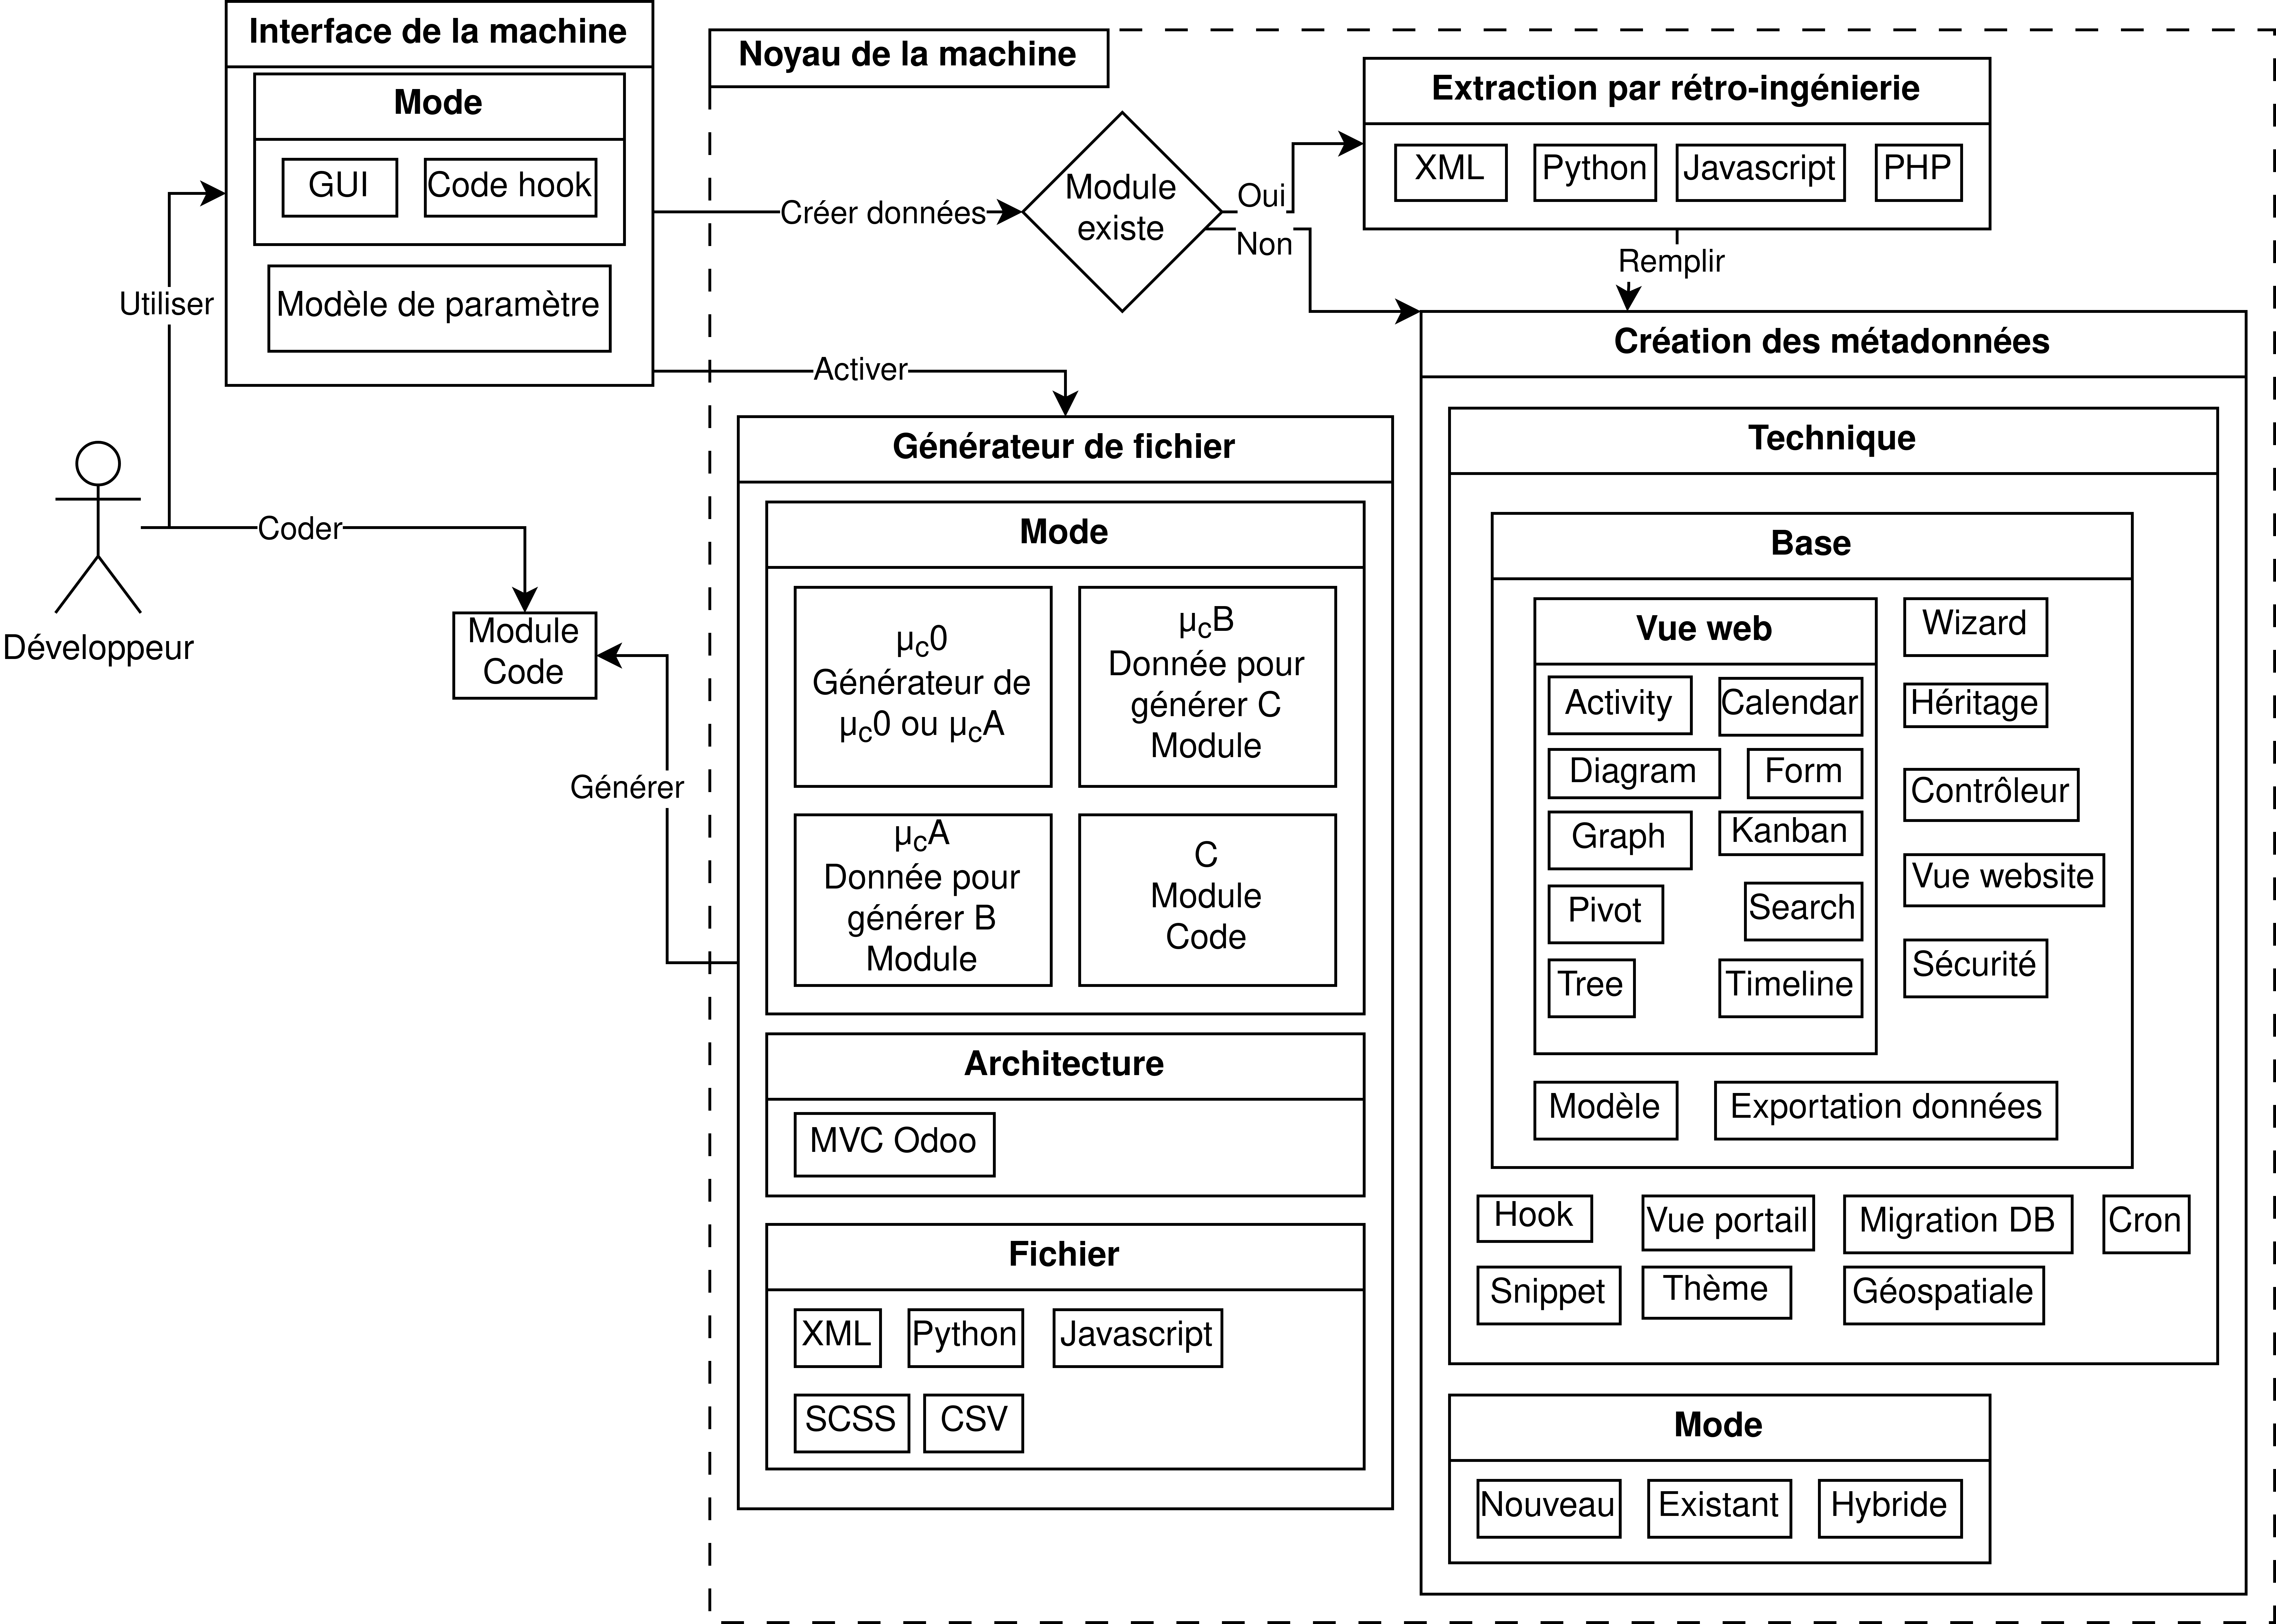
\includegraphics[width=6.535in]{images/architecture_machine.drawio.png}
\caption{Architecture du générateur de code dans son ensemble, nommé machine. Le développeur peut modifier le code source directement ou utiliser l'interface de la machine qui passe par un ensemble de composantes.}
\label{fig:dia_architecture}
\end{figure}

La section de l’interface machine permet à l’utilisateur de créer un modèle de données pour indiquer à la machine quelle opération effectuer avec les données associées. Plusieurs combinaisons, héritables, sont possibles, selon les différentes techniques. De plus, c’est ici que l’on vient activer la génération de code.

La section de l’extraction par rétro-ingénierie permet de remplir le modèle de méta-données, sans passer par la paramétrisation. Ça extrait des informations qui ne sont pas accessibles dans le modèle de données d’Odoo sur le module.

La section de la création de méta-données se fait soit par l’utilisateur via la GUI ou par le «Code \textit{Hook}», il gère simultanément plusieurs techniques qui sont dans des modules. Le mode «nouveau» permet de créer de nouvelles données. Une fois qu’elles sont créées, c’est le mode «existant» qui est utilisé. Cependant, le mode «hybride» permet d’écraser les données existantes en réactivant le mode «nouveau».

La section du générateur de fichiers se fait activer par l’interface, mais prend les méta-données pour faire sa génération, selon le mode qu’il doit générer et l’architecture qu’il connaît. Il fait des liaisons entre les modèles et les vues en référence aux noms des champs de chaque modèle de données.

Chacun de ces blocs de l’architecture est modulaire, chaque technique est héritable, pour modifier le comportement et ajouter des liaisons afin de permettre une génération de code.

La sécurité dépend du modèle, le contrôleur dépend du modèle et la vue dépend du contrôleur et du modèle.

\subsection{Auto-générateur}

On arrive à l'auto-générateur représenté par µ$_C^0$, voir Annexe~\ref{annexe_cg_code_uc0}. Au moment de l'installation de celui-ci, il génère le même code que lui-même, au même endroit dans le système de fichiers. Une légère modification va créer une autre entité qui sera une déviation dans l’objectif de démarrer une chaîne de production logicielle.

C'est le module $M$ qui contient les méta-données de µ$_C^0$. Ainsi, exécuter µ$_C^0$ devient un test de fonctionnalité et on obtient un succès lorsqu'il n'y a pas de différence. Cependant, sa programmation est actuellement spécifique à sa génération, aucun autre module n’a besoin de cette fonctionnalité unique.

L'auto-générateur est utilisé pour générer des µ$_C^A$ avec une légère modification dans les paramètres. Même s'il a la capacité de générer un µ$_C^B$, mieux vaut créer la chaîne proposée pour faire de l'amélioration continue.

\section{Résultats propres à SO-1}
Nous examinerons maintenant les résultats propores à chaque sous-objectif décrit dans le chapitre 3, méthode.
\subsection{Génération par gabarit}

La génération par gabarit était déjà supportée dans la version initiale~\cite{bluiksnot_repo}, de plus, il y a eu des améliorations telles que l'utilisation des \textit{f-strings} au lieu d'utiliser la fonction \textit{format} de \textit{String}, l'utilisation de la bibliothèque Code-writer en Python\footnote{\url{https://pypi.org/project/code-writer/}} et l'utilisation de la bibliothèque lxml\footnote{\url{https://pypi.org/project/lxml/}}.

\subsection{Génération de l'architecture MVC}

L’architecture MVC était déjà supportée dans la version initiale~\cite{bluiksnot_repo}, de plus, il y a eu des améliorations telles que les règles de sécurité sont ajustées selon les configurations et personnalisables par la suite et l'ajout de bouton qui ouvre des \textit{Wizard}\footnote{\url{https://github.com/ERPLibre/odoo-code-generator/tree/9d79f67/code_generator/wizards}} pour générer les vues, les modèles et les contrôleurs, voir Figure~\ref{fig:dia_gui_mvc}, Figure~\ref{fig:dia_wizard_mvc} et le tableau~\ref{tab:stat_code_wizard_mvc} sur les statistiques du code. Ainsi, le développeur peut les configurer et demander de générer les méta-données associées.

\begin{figure}[htb]
\centering
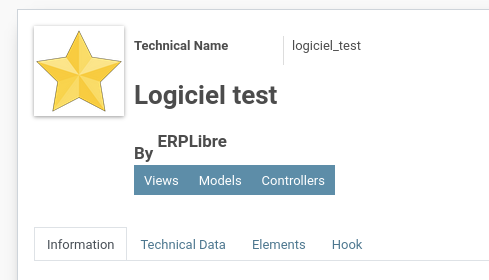
\includegraphics[width=3in]{images/GUI_MVC.png}
\caption{Exemple support MVC dans GUI du générateur de code}
\label{fig:dia_gui_mvc}
\end{figure}

\begin{figure}[htb]
\centering
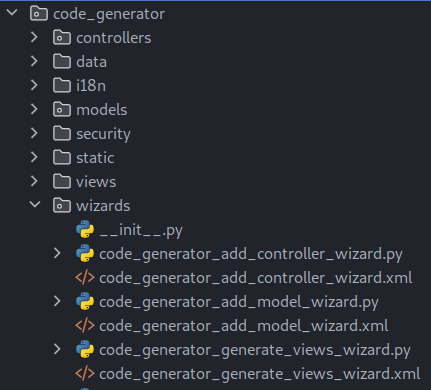
\includegraphics[width=3in]{cg_wizard_mvc.png}
\caption{Démonstration du code pour le MVC dans la section \textit{wizards} du module du générateur de code}
\label{fig:dia_wizard_mvc}
\end{figure}

\begin{table}[htb]
\caption{Statistiques sur le code des «wizards» sur la GUI qui gère la génération de MVC}
\centering
\begin{tabular}{|l|l|l|l|l|l|l|}

\hline
\cellcolor[HTML]{d9d9d9}{\textbf{Langage}} & \cellcolor[HTML]{d9d9d9}{\textbf{Fichiers}} & \cellcolor[HTML]{d9d9d9}{\textbf{\%}} & \cellcolor[HTML]{d9d9d9}{\textbf{Code}} & \cellcolor[HTML]{d9d9d9}{\textbf{\%}} & \cellcolor[HTML]{d9d9d9}{\textbf{Commentaire}} & \cellcolor[HTML]{d9d9d9}{\textbf{\%}}\\\hline

Python & 5 & 55.6 & 1809 & 58.5 & 560 & 17.3\\\hline
XML & 4 & 44.4 & 178 & 92.7 & 10 & 5.2\\\hline
Total & 9 & 100.0 & 2068 & 60.4 & 570 & 16.6\\\hline

\end{tabular}
\label{tab:stat_code_wizard_mvc}
\end{table}

\subsection{Générer un module à partir d’une base de données externes}

La migration de données à partir de SQL était déjà supportée dans la version initiale~\cite{bluiksnot_repo}, cependant il y a eu des améliorations\footnote{\url{https://github.com/ERPLibre/odoo-code-generator/tree/9d79f67/code_generator_db_servers}}, telles que l'ajout de types de données, dont ceux utilisés par le projet Accorderie, l'ajout d'associations entre les types de données et les différentes personnalisations de l’architecture Odoo, la modification de l'interface qui représente la base de données avec les contrôleurs pour permettre la configuration de la migration sur le modèle de données désiré et la gestion des interdépendances entre modèles. Pour gérer le problème d'interdépendances, il a fallut créer une séquence de création des données avec une seule dépendance et, à la toute fin, ajouter l'interdépendance en mettant à jour les données. Il y a eu au moins 1639 ajouts de lignes de code, voir Figure~\ref{fig:dia_cg_db_servers}.

\begin{figure}[htb]
\centering
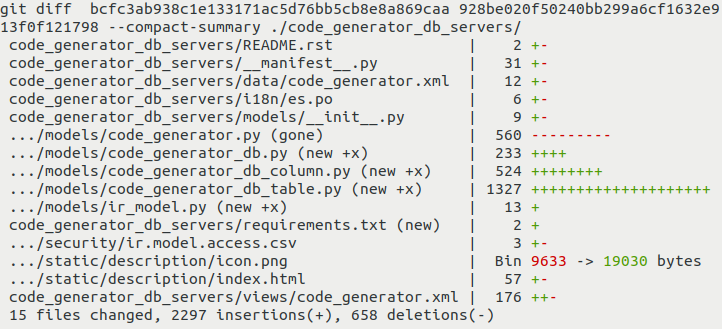
\includegraphics[width=4in]{git_diff_code_generator_db_servers.png}
\caption{Démonstration des modifications effectués pour adapter le code de la migration de base de données pour supporter plus de fonctionnalités.}
\label{fig:dia_cg_db_servers}
\end{figure}

\subsection{Génération de code par des données}

La génération de code par des données a la capacité de prendre les données via les interfaces utilisateurs telles que la GUI et le «Code \textit{hook}». Cela permet la personnalisation pour obtenir un logiciel adapté à ce que l’utilisateur est capable d’exprimer.

Le robot logiciel codeur est une machine qui, grâce à son interface «code \textit{hook}», se fait commander par deux couches de méta-données paramétrables par l’humain. Les deux couches interfèrent entre elles pour permettre l’évolution de la fonctionnalité désirée. Pour voir un exemple de génération de code par données, voir Annexe~\ref{annexe_cg_code_uc0}.

\subsection{Interprétation des résultats de SO-1}

\subsubsection{SO-1 Accomplissements}
Pour résumer l'ensemble des accomplissements du premier sous-objectif (SO-1), nous avons fait une simplification de l’écriture de technique dans le générateur de code avec l’utilisation de \textit{f-string}, de la bibliothèque \textit{Code-writer }et de la bibliothèque \textit{lxml}, nous avons fait un ajout de \textit{Wizard} pour configurer le MVC selon des paramètres, nous avons améliorer l’importation des bases de données externes, supporté la génération de code par des données et augmenté le nombre de techniques de génération de code, le support des \textit{templates} \textit{Qweb} et fait l'ajout du type de données géospatiales.

\subsubsection{SO-1 Feuille de route}
La brève feuille de route du premier sous-objectif se résume à implémenter les fonctionnalités manquantes dans la GUI pour générer les MVC d’un module, à augmenter le nombre de technologies à supporter sur l'importation des données, à ajouter le support de génération sur différentes architectures, à supporter différentes techniques de sécurités personnalisables, comme l’anonymisation des données, à générer automatiquement une documentation sur l’utilisation d’une technique et à supporter la génération sur d’autres systèmes \textit{ERP} libres tel que Tryton\footnote{\url{https://www.tryton.org}}

\section{Résultats propres à SO-2}

\subsection {Extraction de code et reproduction}

De la macro et micro extraction ont été réalisées avec plusieurs techniques combinées. Pour pouvoir faire de la reproduction, il a suffit de faire de la macro extraction, c'est-à -dire faire une recherche dans toutes les classes pour copier le contenu de chaque méthode pour le transformer en méta-données et pouvoir faire l’opération directe de générer le code qui a été copié. L’utilisation de l’\textit{AST} a servi à déterminer quelle ligne de code était à découper pour la recopier.

Cependant, il était nécessaire, dans certains contextes, de faire de la micro extraction, telles que l’extraction des noms des constantes, qui sont transformées en valeurs, lors de l’exécution, l’extraction des commentaires qui n’est pas supportée dans la bibliothèque \textit{AST} de Python 3.7, l’extraction des décorateurs et l’extraction des paramètres sur les méthodes.

De plus, les vues ont été extraites dans le but d'obtenir des méta-données spécifiques qui caractérisent la reconstruction de la vue, ces données n’étaient pas accessibles dans les données d'Odoo.

Tout le code en lien avec l'extraction de données se retrouve dans les fichiers\footnote{\url{https://github.com/ERPLibre/odoo-code-generator/tree/9d79f67/code_generator}} extrator\_controller.py, extractor\_module.py, extrator\_module\_file.py et extractor\_view.py, voir le tableau~\ref{tab:stat_code_extractor} pour comprendre les statistiques sur le code.

\begin{table}[htb]
\caption{Statistiques sur le code de l'extraction de données de modules Odoo}
\centering
\begin{tabular}{|l|l|l|l|l|l|l|}

\hline
\cellcolor[HTML]{d9d9d9}{\textbf{Langage}} & \cellcolor[HTML]{d9d9d9}{\textbf{Fichiers}} & \cellcolor[HTML]{d9d9d9}{\textbf{\%}} & \cellcolor[HTML]{d9d9d9}{\textbf{Code}} & \cellcolor[HTML]{d9d9d9}{\textbf{\%}} & \cellcolor[HTML]{d9d9d9}{\textbf{Commentaire}} & \cellcolor[HTML]{d9d9d9}{\textbf{\%}}\\\hline

Python & 4 & 100.0 & 1415 & 72.6 & 127 & 6.5\\\hline

\end{tabular}
\label{tab:stat_code_extractor}
\end{table}

Certaines informations ont été extraites dans le \textit{Javascript} à l’aide de la bibliothèque \textit{pyjsparser}. Pour l’extraction d'un projet externe d'une autre technologie, un extracteur de PHP a été développé via un \textit{parser} de la communauté\footnote{\url{https://github.com/JameelNabbo/PHP-Parsers}}.

% TODO manque info sur le générateur de générateur de code
C'est en développant les techniques de génération de code que nous réalisons la reproduction. Un script a été développé pour accélérer l’écriture du générateur de code, ainsi qu'un générateur de générateur de code. Ensuite, le développeur peut le transformer légèrement pour prendre les paramètres des méta-données.

\subsection {Amélioration continue sur la génération}

Grâce à l’extraction des méta-données, dès que la technique de génération est bien développée avec les méta-données, le code est automatiquement généré avec de bonnes pratiques logicielles, corrigeant automatiquement les problèmes.

L’intérêt d'utiliser Odoo pour lire le module est qu'il valide déjà certains fonctionnements. Par exemple, il n'y pas d’erreur de syntaxe dans le Python où les XML étaient bien construits.

Ainsi, pour un module désiré, nous utilisons les outils pour générer µ$_C^A$ et µ$_C^B$, puis en avançant dans le développement, nous bouclons entre le 3 et 4 sur Figure~\ref{fig:dia_sequence_gc}.

\subsection {Test de validation de génération de codes}\label{test_validation_generation_code_resultat}

Pour tester ce générateur de code, la technique du test de comparaison des sorties de la génération a été utilisée. Pour procéder, un développeur valide via l'outil Git ce qui est \textit{commité}\footnote{Un terme dans l'outil Git pour valider le code en créant un état dans l'historique.}. Ainsi, un script a été développé pour lancer en parallèle les tests et valider les différences de génération avec ce qui a été \textit{commité} précédemment. Un succès est lorsqu'il y a aucune différence dans le code entre la version générée et la précédente. Ainsi, les tests implémentés permettent de valider l’installation du module généré, de valider que µ$_C^B$ génère bien le module cible sans différence dans le code, de valider que µ$_C^A$ génère µ$_C^B$ sans différence dans le code, ainsi que valider que la migration d’une base de données SQL se fait sans différence dans le code.

En exécutant tous les tests, voir Annexe~\ref{annexe_test_generateur_code}, une couverture de 84\% est obtenue, tous les tests présents sont un succès, sauf ceux sur l’auto-générateur.

Les tests deviennent une documentation sur l'utilisation du générateur de code. Puisque la génération de code se fait par données, il suffit de changer les paramètres pour générer un autre module et lancer un nouveau projet sur le module généré pour obtenir toute la chaîne.

\subsection {Règles de codage standardisées}

Au moment de générer les fichiers, toutes les sorties textes sont traitées par des outils de mise en forme, en suivant des règles de codage standardisées.

Pour le Python, l’outil \textit{black} est utilisé pour la mise en forme en suivant le standard PEP8 avec \textit{isort} pour réordonner les importations. \textit{Black} donne une mise en forme non naturelle comparée à l’écriture de code pour un humain. Cependant, son résultat facilite la lecture et le suivi des différences pour les futurs ajouts. Le Javascript, le HTML et le XML sont mis en forme avec l’outil Prettier.

De plus, le générateur force le déplacement des classes dans leur fichier respectif pour créer une classe par fichier. Les champs, pour chaque modèle, sont déplacés en ordre alphabétique, mais le premier est celui qui est utilisé pour représenter le modèle\footnote{Référence à l'attribut «\_rec\_name»}.

\subsection{Interprétation des résultats de SO-2}

\subsubsection{SO-2 Accomplissements}
Pour résumer l'ensemble des accomplissements du deuxième sous-objectif, nous avons fait de l'extraction du code via l’utilisation d’un AST et extraction des méta-données dans les fichiers XML, de l'amélioration continue sur la génération de code, grâce à la reproduction à l’aide de l’extraction du code, développé un outil pour aider à la création de technique de génération à l’aide d’un générateur de générateur de code, intégré dans le générateur de code des tests de validation en reproduisant l’ensemble des techniques en démonstration, ainsi qu'appliquer des règles de codage standardisées sur la génération de code.

\subsubsection{SO-2 Feuille de route}
La brève feuille de route du second sous-objectif se résume à finaliser l’implémentation de l'auto-génération sur le générateur de code, de mettre à jour les tests pour atteindre une couverture de code à 100\% et d'ajouter des tests sur les techniques d’extractions de code tel que le PHP.

\section{Résultats propres à SO-3}

\subsection{Classification des techniques développées}\label{result_technique_developpe}

En référence à la Figure~\ref{fig:dia_architecture}, les techniques «Modèle», «\textit{Form}», «\textit{Tree}», «Contrôleur» et «Migration \textit{DB}~\footnote{Module de migration de base de données}», étaient déjà implémentées dans la version initiale~\cite{bluiksnot_repo}, mais elles ont reçu des améliorations pour s’agencer aux autres techniques. Les autres techniques ont été développées pour permettre une modularité aux modules à générer, puis supporter de nouvelles fonctionnalités telles que la gestion des cartes interactives avec le géospatial.

% TODO faire un diagramme des dépendances
% Les techniques :
% \begin{enumerate}
%     \item Contrôleur;
%     \item Cron;
%     \item Exportation des données;
%     \item Géospatiale (dépend de Modèle);
%     \item Héritage;
%     \item Hook;
%     \item Migration DB\footnote{importation des données par DB};
%     \item Modèle;
%     \item Portal;
%     \item Sécurité;
%     \item Snippet;
%     \item Thème;
%     \item Vue web;
%     \begin{enumerate}
%         \item Activity;
%         \item Calendar;
%         \item Diagram;
%         \item Form;
%         \item Graph;
%         \item Kanban;
%         \item Pivot;
%         \item Search;
%         \item Timeline;
%         \item Tree;
%     \end{enumerate}
%     \item «website\_leaflet» (dépend de Snippet et Géospatiale);
%     \item Wizard;
% \end{enumerate}

\subsection{Interface du générateur de code}

\subsubsection{L'interface graphique}

 L'interface graphique existait déjà dans la version initiale~\cite{bluiksnot_repo}, elle a été améliorée pour afficher plus d'informations par rapport au développement. Elle sert à faciliter la paramétrisation du générateur de code. Elle n’a pas été priorisée et elle manque de fonctionnalités si nous la comparons à ce qui peut être supporté via la technique \textit{code hooks} avec µ$_C^A$ et µ$_C^B$. L'interface permet de créer un module, de renommer un module, d'ajouter des modèles, voir Annexe~\ref{annexe_cg_gui_model}, et des champs, voir Annexe~\ref{annexe_cg_gui_champs}, d'ajouter des menus, d'ajouter de la sécurité, de changer les icônes, de changer les informations sur les propriétés \textit{manifest }du module, d'ajouter du code, voir Annexe~\ref{annexe_cg_gui_code} et de modification des \textit{hooks}, voir Annexe~\ref{annexe_cg_gui_hook};

\subsubsection{L'interface \textit{code \textit{hook}}}

L'interface \textit{code \textit{hook}}, voir exemple à l'Annexe~\ref{annexe_cg_code_uc0}, permet d’accéder à la totalité des fonctionnalités du générateur de code via µ$_C^A$ et µ$_C^B$. Elle a été utilisée pour toutes les démonstrations qui servent de tests et elle contient la paramétrisation pour les modules désirés. De plus, l'avantage de cette interface est qu'elle nous permet d'ajouter du code pour rendre dynamique la paramétrisation.

\subsection{Interprétation des résultats de SO-3}

\subsubsection{SO-3 Accomplissements}
Pour résumer l'ensemble des accomplissements du troisième sous-objectif, nous avons fait l'ajout de nouvelles techniques et une classification de celles-ci, nous avons rendu accessible une interface graphique pour paramétrer la génération de code et avons rendu accessible une interface de programmation pour utiliser toutes les fonctionnalités du robot logiciel codeur.

\subsubsection{SO-3 Feuille de route}
La brève feuille de route du troisième sous-objetif se résume à ajouter des paramètres pour faire davantage de personnalisation sur les techniques, à extraire les techniques du générateur et les implémenter une par module, à supporter les fonctionnalités manquantes sur toutes les techniques pour l’interface graphique et à supporter l’accès à la création de méta-données par la rétro-ingénierie via l’interface graphique.

\section{Résultats propres à SO-4}

\subsection{Utilisation d’un conteneur Docker}

Puisque le générateur de code fait partie de ERPLibre, la version 1.5.0 contient les modules de génération de code. Le déploiement se fait rapidement en utilisant le logiciel Docker et le générateur de code permet l’utilisation de l’interface graphique pour générer des modules Odoo.

\subsubsection{SO-4 Feuille de route}
La brève feuille de route du quatrième sous-objectif se résume à développer une synchronisation entre les instances pour permettre la redondance, à développer une gestion de son infrastructure via le générateur de code, à faire participer le robot logiciel codeur à la maintenance de l’infrastructure de déploiement, à utiliser d’autres systèmes de conteneur en distribution qui sont libres comme «\textit{Pod}»~\footnote{\url{https://podman.io/}} et à développer la capacité du robot logiciel codeur de valider techniquement si le logiciel est AGPLv3 au moment de l’exécution.

\section{Résultats propres à SO-5}
Le cinquième sous-objectif met en relation le générateur de code avec la communauté. Le but du générateur de code n'est pas de remplacer les humains, mais de mieux les outiller et soutenir la communauté. De plus, le cinquième sous-objectif présente les deux cas d'étude propres à ce mémoire.
\subsection{Guide : créer une communauté autour d’une technologie pour un réseau d’entraide libre}

% Un guide hybride a été produit pour comprendre les aspects cités du démarrage d’un projet, de gestion d’une communauté autour d’un projet libre et des règles d'hébergement libres. 

Avant de démarrer un projet, nous suggérons au gestionnaire de projet de suivre le guide en 7 étapes, voir Annexe~\ref{annexe_demarrer_projet_7_etape}, qui permet de démarrer rapidement un projet et de s'assurer que les membres impliqués du réseau d'entraide comprennent les mêmes enjeux et s'alignent dans la même direction. Par la suite, nous proposons le guide suivant pour gérer l'intégration d'un membre en communauté, voir Annexe~\ref{annexe_guide_integration_membre}. De plus, nous encourageons les bonnes habitudes en communauté avec le guide suivant pour la gestion du comportement en communauté, voir Annexe~\ref{annexe_guide_comportement}. Ensuite, pour se préparer au développement public, nous conseillons le guide suivant, voir Annexe~\ref{annexe_guide_dev_public}. Les problèmes peuvent survenir entre les membres de la communauté, c'est pourquoi nous suggérons le guide suivant pour faciliter la résolution de problème, voir Annexe~\ref{annexe_guide_resolution_probleme}. La communauté a besoin ensuite de formation technique et fonctionnelle, voir Annexe~\ref{annexe_guide_documentation}. Puis la sécurité est importante pour protéger les données dans la communauté, ce pourquoi nous suggérons les étapes suivantes à intégrer au projet communautaire, voir Annexe~\ref{annexe_guide_securite}. Puis au niveau de la communication, nous suggérons de faire un suivi des émotions et des sentiments des membres lors des réunions relatives au projet et mettre en place des outils favorisant la communication non violente. Finalement, en lien avec le développement libre, nous suggérons les étapes suivantes, voir Annexe~\ref{annexe_guide_libre}.

% \section{Projets divers}

\subsection{Projet module «auto\_backup»}

Le module «auto\_backup»\footnote{\url{https://github.com/ERPLibre/server-tools/tree/f6054fc/auto_backup}} est le premier module de la communauté de l'organisation OCA répertoire \textit{server-tools} à avoir été testé dans ce projet, un µ$_C^A$\footnote{\url{https://github.com/ERPLibre/odoo-code-generator-template/tree/b5ae8e/code_generator_template_demo_sysadmin_cron}} et µ$_C^B$\footnote{\url{https://github.com/ERPLibre/odoo-code-generator-template/tree/b5ae8e/code_generator_auto_backup}} ont été générés. Le générateur de code a pu modifier le module pour appliquer de la qualité logicielle qui a permis de développer la technique de gestion des \textit{cron}, en lançant des sauvegardes, par SSH ou en local, à des moments spécifiques dans le temps.

% \subsection{Projet module \textit{workflow} \textit{design}}

% C’est un module de gestion de projet qui a été développé entièrement avec le générateur de code qui permet de faire le suivi sur les opportunités, les menaces, les forces, les faiblesses et les objectifs. Il a été utilisé dans le projet Accorderie.

% \subsection{Projet module STARS}

% Le module STARS dépend de l’application Projet, il permet de configurer une procédure intégrée dans un projet pour suivre les étapes de STARS, voir Figure~\ref{fig:workflow_stars}.

% \begin{figure}
% \centering
% 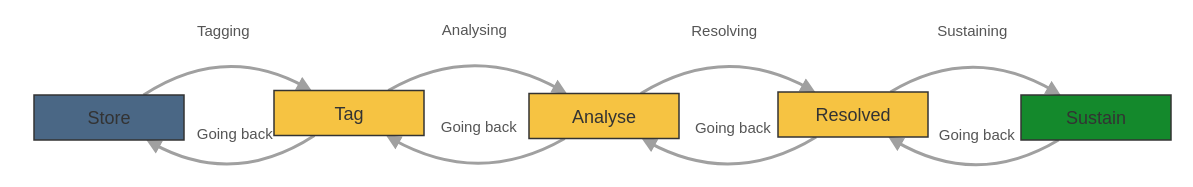
\includegraphics[width=6.535in]{workflow_stars.png}
% \caption{Procédure STARS dans l'application Projet vue Diagramme}
% \label{fig:workflow_stars}
% \end{figure}

% Ainsi, nous pouvons créer un nouveau projet et suivre cette procédure en ajoutant des tâches d'amélioration continue de son organisation, voir Figure~\ref{fig:kanban_stars}.

% \begin{figure}
% \centering
% 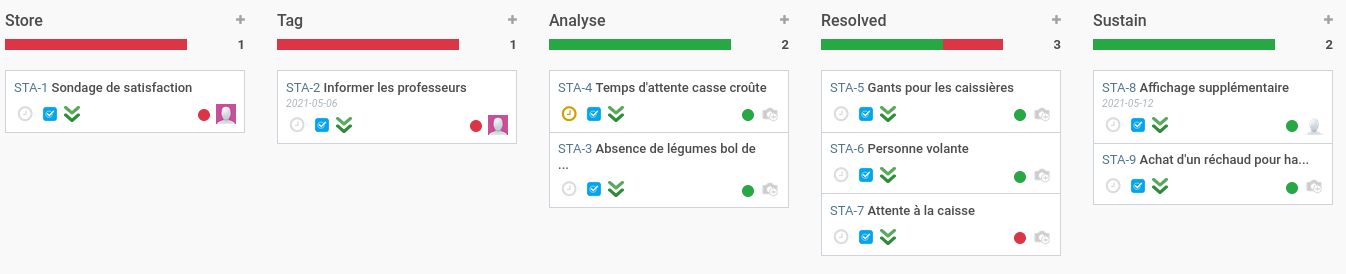
\includegraphics[width=6.535in]{kanban_stars.png}
% \caption{Suivi des tâches de projet avec procédure STARS en vue Kanban}
% \label{fig:kanban_stars}
% \end{figure}

\subsection{Projet module SRS}

Le module de spécification des exigences logiciels (SRS), c’est un module de gestion de projet qui a été développé entièrement avec le générateur de code\footnote{\url{https://github.com/ERPLibre/scrummer/tree/45ef25/code_generator_project_srs}}\footnote{\url{https://github.com/ERPLibre/scrummer/tree/45ef25/code_generator_template_project_srs}}\footnote{\url{https://github.com/ERPLibre/scrummer/tree/45ef25/project_srs}}. Il permet de faire l’analyse des besoins pour ensuite passer à l’analyse fonctionnelle et, finalement, définir les requis fonctionnels d’un projet. Il a été utilisé, entre autres, pour le projet Accorderie et le projet Portail CEPPP.

\subsection{Projet espace Accorderie}

Le projet\footnote{\url{https://github.com/TechnoLibre/odoo_accorderie/tree/ae5b4c}} a débuté par l'élaboration d'une analyse des besoins fonctionnels, puis un ensemble de requis logiciels ont été rédigés avec un membre du Réseau de l'Accorderie.

Le générateur de code a permis de créer un module Odoo 12.0 avec les modèles de données de l'Accorderie calqués sur leur base de données en SQL de MariadB, voir Annexe~\ref{annexe_db_accorderie_2019}.

Plusieurs corrections ont été effectuées avant la migration : correction des noms des champs pour les uniformiser; correction des types de champs (exemple le «\textit{True}» était exprimé par la valeur «-1» dans un type «\textit{int}», ainsi ce type a été transformé en booléen); enlever les doubles dépendances par changement de l’architecture; correction des données erronées (un champs est requis, mais il manque des données pour certaines entrées). De plus, le modèle de données n’a pas été conçu pour de l’automatisation, mais plutôt pour que les échanges de services soient validés par des membres de la communauté.

Dans l'Annexe~\ref{annexe_db_accorderie_2023}, on peut observer les adaptations des champs. Par exemple, avec la table «accorderie\_echange\_service», il y a l'ajout des champs : «nb\_heure\_estime» pour avoir une prévision des heures à effectuer, «nb\_heure\_dure\_trajet» pour reconnaître le temps de déplacement, «distance\_trajet» pour connaître la distance qui sera calculée avec le projet libre \textit{Open Source Routing Machine} (OSRM).

La migration du modèle de données a été faite dans un module qui dépend de la technique \textit{Migration DB }qui permet d'importer le modèle. Certaines données nécessitent la création d’un fichier de données XML. Pour les autres données, un autre module a été créé pour ajouter les données directement dans une base de données qui sera migrée vers une mise en production.

Un portail a été généré, pour remplacer les formulaires utilisés par l'ancienne plateforme PHP pour visualiser les entrées. Cependant, cette fonctionnalité a été abandonnée, puisque cette technologie ne plaisait pas.

Une maquette a été conçue pour un nouvel espace membre. Ainsi, nous avons utilisé la technique \textit{website\_snippet} pour afficher des données sur le site web et créer des formulaires. Cette base a permis d’accélérer la création de code de communication entre le client et le serveur. À force de faire l’intégration et la personnalisation de cette maquette, il n’y a plus vraiment de code qui provient du générateur de code.

Le générateur de code a permis d’aider à créer un diagramme pour afficher le processus d’échange de temps, voir Annexe~\ref{annexe_processus_accorderie_2023}, puis une application en Javascript avec AngularJS a été développée pour afficher ce processus à l’utilisateur, une machine à état, qui permet de revenir, selon des paramètres, à un état du processus.

Dues à des limitations humaines et de temps, tout le reste du projet a dû être fait manuellement, puisque la technologie a été changée pour faciliter le développement de l’interface.

Les statistiques du travail sont démontrées dans le tableau~\ref{tab:stat_code_accorderie}.


\begin{table}[htb]
\caption{Statistiques sur l'ensemble des modules Odoo pour le projet Accorderie.}
\centering
\begin{tabular}{|l|l|l|l|l|l|l|}

\hline
\cellcolor[HTML]{d9d9d9}{\textbf{Langage}} & \cellcolor[HTML]{d9d9d9}{\textbf{Fichiers}} & \cellcolor[HTML]{d9d9d9}{\textbf{Code}}\\\hline

XML & 79 & 34711\\\hline
Python & 91 & 19434\\\hline
Javascript & 14 & 3755\\\hline
Css & 37 & 2488\\\hline
Autre & 3 & 57\\\hline
Total & 224 & 60445\\\hline

\end{tabular}
\label{tab:stat_code_accorderie}
\end{table}

\subsection{Projet Portail CEPPP}

Dans le second cas d'étude pour le Projet Portail CEPPP, l'objectif était de faire une section portail pour les patients et une section administrative pour les recruteurs, les partenaires et les administrateurs de la plateforme, de rendre accessible des formulaires et d'anonymiser les données. Le mandat était de migrer les fonctionnalités de la plateforme qui a été développée sur SuiteCRM en PHP.

Un module d'extraction de PHP a été développé, mais il n'est pas accessible dans les techniques du générateur de code. Le modèle de données était directement dans le code et, puisqu'il est dynamique, il n'est pas dans la base de données. La base de données n'a pas été extraite, les données ont été exportées en \textit{Comma-separated values} (CSV) et un module d'importation des données a été développé. Au total, il y a eu 23 fichiers analysés et 2851 données extraites.

Voici les statistiques du Tableau~\ref{tab:stat_code_portail_ceppp} du code après ré-ingénierie et adaptation des fonctionnalités à livraison de la plateforme en début septembre 2023\footnote{\url{https://portailppp.ca}}.

\begin{table}[htb]
\caption{L'évolution entre la génération et la ré-ingénierie des statistiques sur les langages du portail CEPPP}
\centering
\begin{tabular}{|l|l|l|l|}

\hline
\cellcolor[HTML]{d9d9d9}{\textbf{Langage}} & \cellcolor[HTML]{d9d9d9}{\textbf{\# Ligne extrait}} & \cellcolor[HTML]{d9d9d9}{\textbf{\# Ligne personnalisée}} & \cellcolor[HTML]{d9d9d9}{\textbf{\# Diff}}\\\hline

XML & 6 861 & 3 856 & - 3 005\\\hline
Python & 567 & 1 564 & + 997\\\hline
Javascript & 0 & 68 & + 68\\\hline
CSV & 25 & 51 & + 26\\\hline

\end{tabular}
\label{tab:stat_code_portail_ceppp}
\end{table}

L'anonymisation n'est pas supportée par le générateur de code, puis la personnalisation enlève beaucoup de champs mis de manière générique dans les fichiers XML. 

Le modèle de données du portail CEPPP dans Odoo 12 contient 24 modèles Annexe~\ref{annexe_db_ceppp_2022}. L'interface administrateur Annexe~\ref{annexe_form_ceppp_2022} contient la fiche du patient dont les partenaires ont accès seulement qu'à la partie anonymisée Annexe~\ref{annexe_form_anonyme_ceppp_2022}.

Le nombre de lignes de XML a diminué car le générateur de code génère, de base, toutes les vues de tous les champs. Au moment de la ré-ingénierie, il y a eu beaucoup de nettoyage et de données XML effacées. Cependant, le développeur va mettre plus de code Python pour développer des logiques qui ne sont pas supportées par le robot logiciel codeur. Le Javascript ajouté sert à supporter les dates dans le portail. L’ajout de CSV permet l’ajout de permissions et rôles pour l’anonymisation.

\subsection{Interprétation des résultats de SO-5}

\subsubsection{SO-5 Accomplissements}
Pour résumer l'ensemble des accomplissements du cinquième sous-objectif, nous avons fait un test de la génération sur un module existant de la communauté nommé «auto\_backup», des modules de gestion de projet ont été générés pour faire le suivi de la conception fonctionnelle et de l’amélioration continue, le projet Accorderie a bénéficié du générateur de code pour la migration de la base de données vers Odoo et le projet Portail CEPPP a bénéficié du générateur de code pour la migration du code PHP vers Odoo, ainsi que de l’aide au développement de la section Portail.

\subsubsection{SO-5 Feuille de route}
La brève feuille de route du cinquième sous-objectif se résume à supporter la demande de \textit{\textit{Pull Request}} sur les projets Git respectifs, lorsqu’il y a une amélioration. Il doit y avoir un suivi et valider les règles de contribution de la communauté, développer d’autres modules de gestion de projet pour l’accompagnement dans le développement de projet client, développer des modules de gestion de communauté sur des projets de logiciels libres et créer le suivi du développement des modules communautaires avec une traçabilité sur les résultats avec des métriques de génie logiciel.

\section{Discussion}

\subsection{Comment les résultats obtenus soutiennent-ils le libre?}
Le réseau d’entraide a besoin d’un support technologique libre, puisque permettre aux participants de suivre leurs 4 libertés vont faciliter l'adaptation à des situations d’urgence et apporter des solutions rapidement. Les 4 libertés sont : étudier, copier, modifier et utiliser. La liberté d'étudier est représentée par la rétro-ingénierie qui a permis au générateur de code de comprendre certaines fonctionnalités pour pouvoir recréer les méta-données adéquatement pour la reproduction. La liberté de copier est représentée par l’auto-générateur qui a été mis en place, il reste à auto-reproduire le robot logiciel codeur, par son module principal de générateur de code. La liberté de modifier est représentée au moment d'une ré-ingénierie, la rétro-ingénierie est accessible pour permettre une génération de code automatique en appliquant une mise en forme de code et une validation de la qualité logicielle. Puis la liberté d'utiliser est représentée par le robot logiciel codeur qui a la capacité d’utiliser ses fonctionnalités générées et d’exécuter des scripts d’automatisation à des périodes de temps adaptables.

\subsection{Avancement sur le développement en réseau d'entraide}

Voir Figure~\ref{fig:dia_outil_dev_reseau_entraide}, un ensemble d'outils est rendu accessible aux gestionnaires de communauté, aux développeurs de projet. L'outil \textit{No-code/Low-code} est l'interface du générateur de code pour les assister dans leur développement. La section formation sur le développement comprend les exemples de code via les tests qui sont faits pour être facilement transformables pour gérer des nouveaux contextes. La détection des anomalies est mise en place par la révision par les pairs sur l'état du code. Des guides de gestion de communauté sont accessibles pour faciliter l'ajout de participants. Enfin, la mise en place de méthodologie Agile avec suivi du développement pour l'adaptation aux changements est mise à disposition.

\begin{figure}
\centering
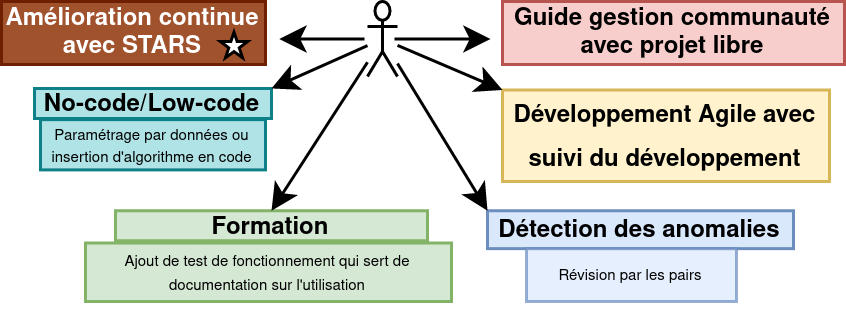
\includegraphics[width=5in]{images/developpeur_outil_developpement.drawio.png}
\caption{Intéraction entre les développeurs et les outils de développement dans un réseau d'entraide}
\label{fig:dia_outil_dev_reseau_entraide}
\end{figure}

\subsection{Avancement de la technopoïèse}\label{avancement_technopoiese}
Voir Figure~\ref{fig:dia_auto_machine_discussion}, la ré-ingénierie manuelle est le processus habituel d'un développeur. Avec ce projet, nous avons une autopoïèse fonctionnelle semi-automatique, avec intervention humaine, puis une allopoïèse complète avec intervention humaine, lorsque cette dernière est en dehors des techniques maîtrisées par le robot logiciel codeur.

Pour l'Allopoïèse, le robot logiciel codeur vient assister l'intervention humaine à $H_0$ et $H_1$, qui permet de passer des méta-données, sur le module désiré, à une nouvelle version de ce module. Après une modification, il faut boucler avec le mode direct et le mode indirect du générateur de code pour avoir une version stable.

Pour l'Autopoïèse, la génération de code se fait directement sur le module de génération de code, c'est-à-dire que la machine est mise à jour avec l'assistance de la machine. L'humain intervient dans l'adaptation de la fonctionnalité et la correction de technique d'ingénierie au moment de la génération, aux endroits $H_0$ et $H_1$. À la fin de la modification, il faut boucler avec le mode direct et le mode indirect du générateur de code pour avoir une version stable de soi-même. Puisque le générateur de code génère le générateur de code, il y a des techniques et guides d'utilisation qui sont mis à la disposition dans le projet pour éviter de s'auto-écraser\footnote{C'est un problème qui peut arriver fréquemment dans ce système, de perdre des modifications en bouclant dû à une mauvaise manipulation ou une mauvaise configuration. Il faut toujours \textit{comiter} le travail avant de démarrer la machine.} et perdre son travail.

\begin{figure}
\centering
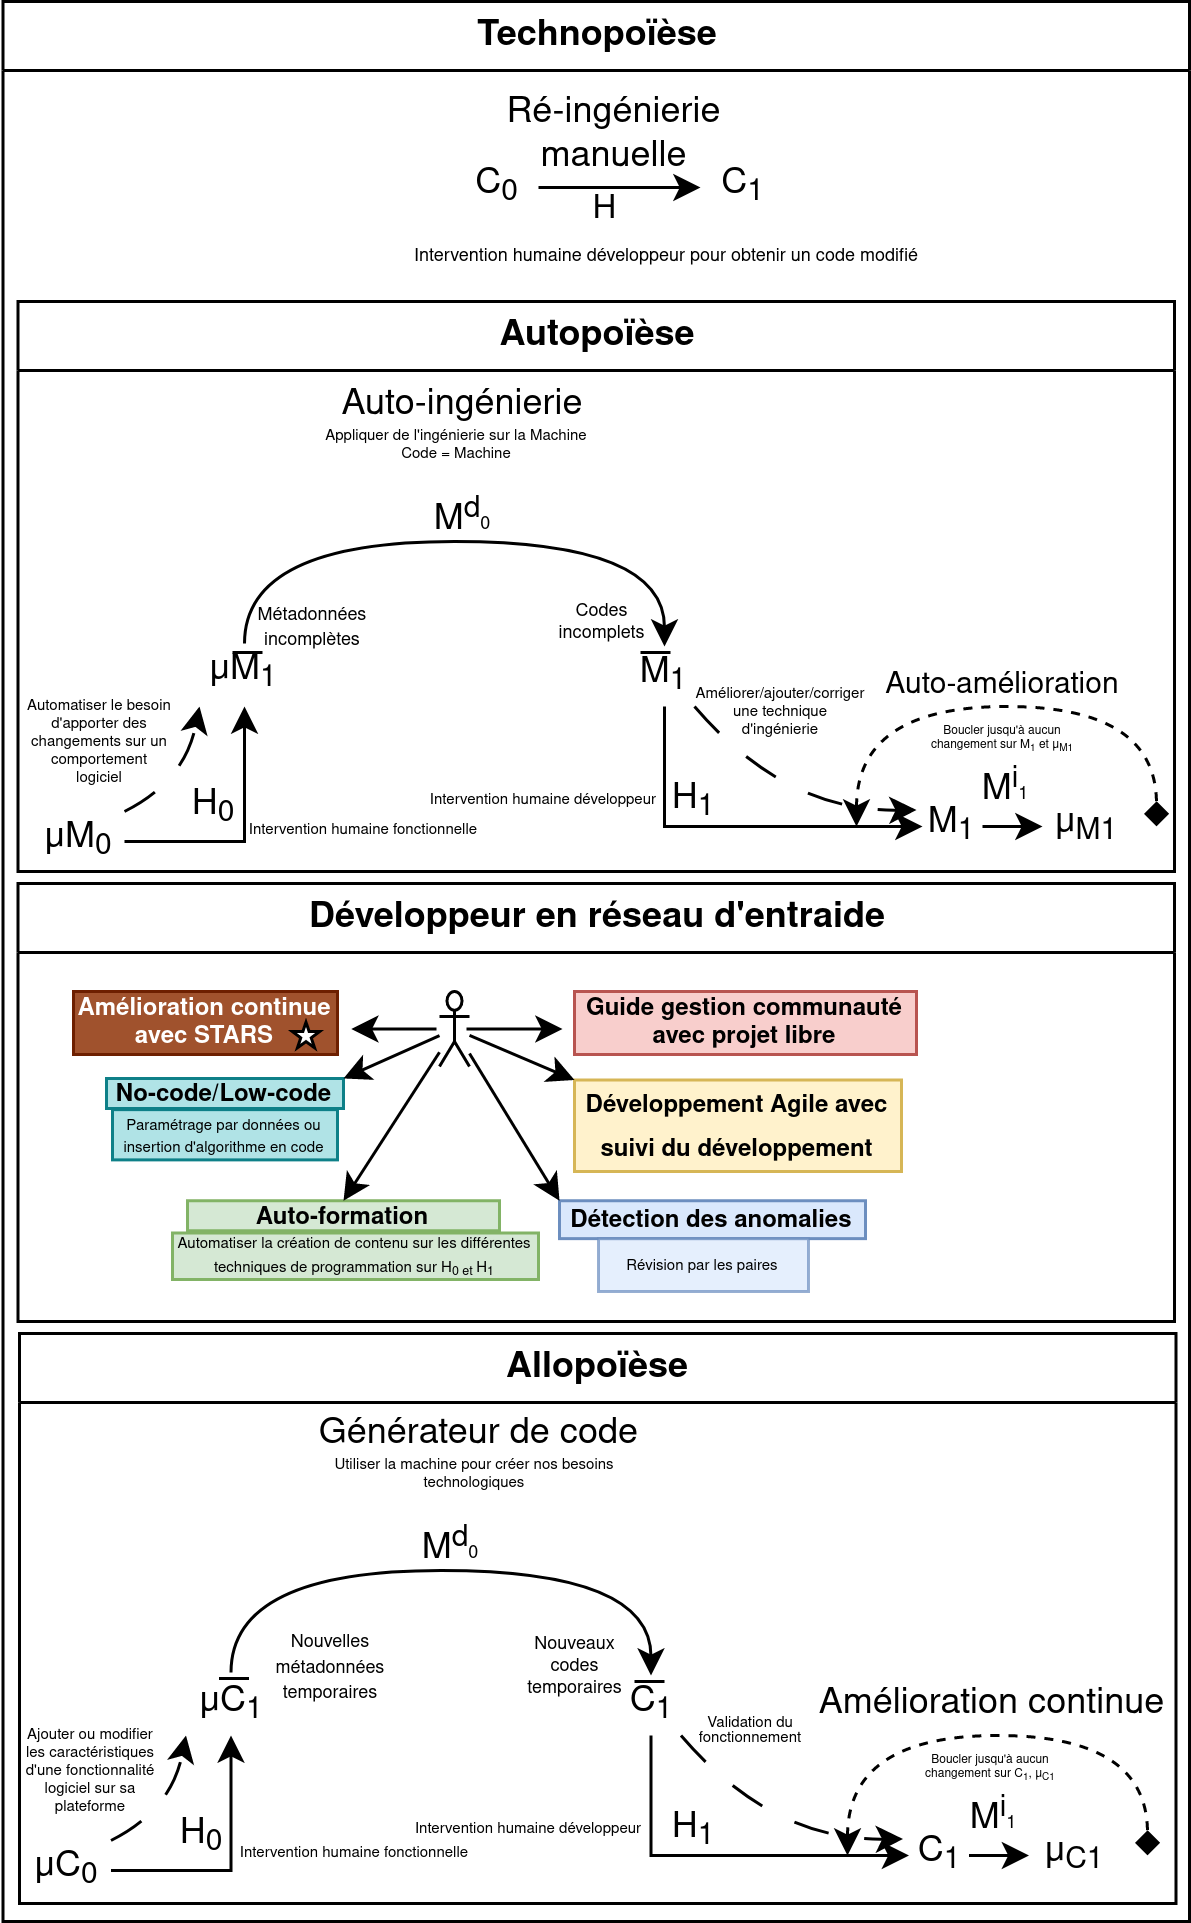
\includegraphics[height=8.5in]{images/auto_machine_discussion.drawio.png}
\caption{Architecture du générateur de code}
\label{fig:dia_auto_machine_discussion}
\end{figure}

\subsection{Réalisation du robot logiciel générateur de code}
Dans la revue littérature section~\ref{robot_logiciel_developpeur_revue}, nous avons déterminé 4 critères pour définir un robot logiciel codeur :

\subsubsection{Autonomie}
Nous avons des résultats qui démontrent 100\% d'autonomie dans quelques contextes, voir les résultats sur les tests de validation Section~\ref{test_validation_generation_code_resultat}. Cependant, le robot logiciel codeur n'est pas 100\% autonome pour tous les contextes, il a besoin d'intervention humaine pour des personnalisations ou des techniques non supportées, voir Section~\ref{avancement_technopoiese}.

% TODO une fois qu'on aura supporté plus de technique et l'autopoïèse entière, la prochaine étape serait de le faire fonctionner en continue. Bien qu'il soit capable via l'interface graphique, les efforts n'ont pas été effectué pour cette capacité.

\subsubsection{Adaptable}
Le robot logiciel codeur est adaptable, il génère 6 composantes, voir résultat d'architecture section~\ref{architecture_result} : web, \textit{website}, portail, \textit{snippet}, migration de données entrantes et migration de modèle de données entrantes. De plus, il est capable d'interagir avec des technologies en dehors d'Odoo comme extraire du code externe en PHP du logiciel SuiteCRM et des bases de données externes (MySQL/SQL Server/PostgreSQL) pour importer des modèles de données et migrer des données.

% TODO il faudrait supporter la génération de technologies externes, nous travaillons présentement à générer des applications mobiles natives, ou même générer des modules sur d'autres plateforme ERP tel que Tryton ou NextERP.

\subsubsection{Compétences techniques}
Le robot logiciel codeur contient plusieurs compétences techniques qui sont décrites dans les résultats section~\ref{result_technique_developpe}. De plus, il permet la personnalisation pour chacune des composantes du nombre de champs, des types de champs et du type d'affichage associé aux champs.

% TODO les techniques ont été développés comme preuve de concept, il manque de mâturité et de personnalisation. 

\subsubsection{Compétences sociales}
Le robot logiciel codeur donne accès à des outils pour le développeur. Il y a une interface graphique LCNC qui permet la paramétrisation pour la génération de code. Il y a aussi une interface de code pour paramétrer le fonctionnement de la génération accompagnée de la rétro-ingénierie et il permet d'accompagner le développeur dans l'évolution de son module. Il contient aussi une fonctionnalité pour afficher les différences de code entre la version précédente et la version générée, il permet de créer des statistiques sur les lignes de codes et il permet de montrer la couverture de code.

% TODO manque l'outil en temps réel, ce n'est pas supporté dans Odoo, il faut utiliser une application tierce tel que Etherpad et ajouter les méthodes de synchronisation des mises à jour sur les données. Il manque l'accès directe aux script à la racine du projet ERPLibre pour contrôler les outils de contrôle de la qualité. Collaboration, conscience professionnelle, résolutions de problèmes en équipe, communication efficace, adaptivité sur les livrables et exigences clientes



% \subsection{DevOps}
% Il faudrait mettre en place les outils de dev ops.
% Mise à jour des bibliothèques (avoir une vue d’ensemble autre que Poetry)

% \subsection{Gestion de communauté}
% Un downtime de plus d’une journée cause drastiquement un abandon des participants à l’utilisation d’une technologie au sein d’une autre.

% \subsection{Réseau d’entraide}

% Il doit y avoir un responsable pour chaque localité accompagné du robot logiciel codeur pour répondre à ses besoins de numérisations via une souveraineté numérique. C’est le gestionnaire de communauté.

% Chaque projet d’urgence doit être capable d’avoir une équipe en charge pour accélérer la résolution de problèmes locaux.

% \subsection{Technopoïèse}
% À titre de discussion sur la signification de technopoïèse.

% Auto-répliqueur : une machine qui se copie lui même.
% Allopoïèse : une machine qui crée une autre machine avec des éléments extérieurs, l’inverse de l’autopoïèse.
% Autopoïèse : la propriété d’un système de se produire lui-même, en permanence et en intéraction avec son environnement, et ainsi de maintenir son organisation (structure) malgré son changement de composants (matériaux) et d’informations (données).
% REF https://fr.wikipedia.org/wiki/Autopo%C3%AF%C3%A8se
% Technopoïèse : une technologie qui a la propriété de se produire lui-même …
% «Une technologie pour étudier la vie humaine, des nouvelles sociétés et les accompagner dans leur développement d’autopoïèse. »
% La technopoïèse doit être développée dans un contexte de logiciel libre pour mettre au centre le réseau d’entraide et avoir le contrôle sur les dérives non éthiques.
% Outil passif utilisé par les humains pour jouer un rôle actif dans la création de la société et de la culture en façonnant leur environnement et leur mode de vie. Comprendre comment les technologies influencent la façon dont les individus interagissent et comment elles peuvent être utilisées pour améliorer la vie des gens, de manière responsable et éthique.

% \subsection{robot logiciel codeur libre}

% Les robots codeurs peuvent être programmés pour effectuer différentes tâches, telles que la génération de code source, la correction de bugs, l'optimisation des performances, la maintenance des systèmes et la gestion de versions. Certains robots codeurs peuvent même apprendre à partir d'exemples de code existant et développer des algorithmes en se basant sur des données d'entrée.

% Les robots codeurs peuvent également améliorer la qualité du code en réduisant les erreurs humaines, en accélérant les tests et en appliquant des pratiques de codage cohérentes.»

% TODO projet d’impression 3D à distance, avec des propriétaires de machines qui les entretiennent.

% TODO connaissance de la physique et les appliquer, optimisation pour accompagner les communautés dans leur gestion d’urgence
% TODO doit reproduire les 4 libertés pour l’utilisation, l’accompagner dans son développement pour améliorer ses habitudes de vies par lui même sans dépendre d’autrui, restons en communauté locale pour réduire la consommation.
% TODO faciliter l’intégration de l’intération entre notre robot personnel et celui d’une technologie externe.

             % Second thème (Doctorat) ou "Résultats théoriques et expérimentaux" (Maîtrise) / Second theme (PhD) or "Theoretical and experimental results" (Master's)
\Chapter{CONCLUSION}\label{sec:Conclusion}
% Texte / Text.

%%
%%  SYNTHESE DES TRAVAUX / SUMMARY OF WORKS
%%
\section{Synthèse des travaux}
% Texte / Text.
Les résultats obtenus ont permis d’atteindre en tout ou en partie l’ensemble des sous-objectifs énoncés dans le chapitre~\ref{chapitre_methode}.%, voir Tableau~\ref{tab:synthese_travaux}.

\subsection{Projet Accorderie}
% TODO synthèse
La migration de la base de données a été réussie, mais elle est encore à ce jour en adaptation vers un modèle Odoo plus intégré au ERP. Les efforts ont été mis pour la création d’une interface utilisateur avec des technologies qui n’étaient pas à la base supportées dans Odoo.

\subsection{Projet Portail CEPPP}
% Synthèse
La signification que le nombre de lignes de XML aurait diminué, c’est que l’automate génère de base toutes les vues de tous les champs. Au moment de la ré-ingénierie, il y a eu beaucoup de nettoyage et de données XML effacées. Cependant, le développeur va mettre plus de code Python pour développer des logiques qui ne sont pas supportés par l’automate. Le Javascript ajouté sert à supporter les dates dans le portail. L’ajout de CSV sert pour l’ajout de permissions et rôles pour l’anonymisation.

Après la première migration par l’extraction du modèle de données par PHP, le client a pu testé la plateforme pour avoir une idée à quoi ressemblerait l’utilisation dans l’espace administration de leur modèle de données et ils ont fait des demandes de changement. Une analyse a été effectuée, nous avons utilisé le générateur de code pour générer les vues portails et fait une ré-ingénierie manuelle du modèle et des vues pour obtenir le résultat désiré. Une des fonctionnalités implémentés est l’anonymisation des données pour certains groupes d’utilisateurs, pour pouvoir visualiser des données sans avoir d’information personnelle sur le patient.




%%
%%  LIMITATIONS
%%
\section{Limitations de la solution proposée}\label{sec:Limitations}
% TODO dire en quoi ce que tu as fait améliore l’état de l’art décrit dans la littérature SYNTHÈSE
% TODO décrire les limitations/faiblesses de ce que tu as produit comme logiciel/résultats LIMITATION

\subsection{Couverture des tests}
% TODO limitation
Les tests devraient couvrir 100\% du code, cependant la couverture est de 84\% pour 3 raisons :

\begin{enumerate}
    \item Il y a du code fonctionnel non testé, il manque des tests;
    \item Il y a du code désuet qu’il faut nettoyer ou refactoriser;
    \item La gestion des erreurs n’est pas couverte, il faudrait les ignorer dans le test de couverture et faire des tests unitaires qui valide la gestion des erreurs.
\end{enumerate}


%%
%%  AMELIORATIONS FUTURES / FUTURE RESEARCH
%%
\section{Améliorations futures}
% Texte / Text.
% TODO dire ce qui doit être fait pour que les aspects d’utilisabilité de ton logiciel en terme de communauté, de libre, etc soient complets.

% TODO parler de la sympoïèse comme étant la suite sur la partie communautaire et la distribution de système


\subsection{Amélioration du générateur code}
% TODO amélioration future
Il faut intégrer la génération de code à l’intérieur des instances clientes dans l’objectif qu’ils soient accessibles de son gestionnaire de déploiement pour y ajouter les nouvelles fonctionnalités, démarrer la mise à jour, les tests, les améliorations, la migration, importation. Les instances clientes devraient proposer aux clients via les interfaces 

% Intégration de plusieurs types de réseaux de neurones accessibles librement, il doit être compatible avec le libre.

% Il faut suggérer aux clients des améliorations et de communiquer avec leurs gestionnaires de déploiements.

% Un générateur de code a été créé. L’embryon est créé, il faut terminer sa génération du générateur de code. Les déviances sont déjà créées

Une fois que le générateur de code aura atteint 100\% d’auto-génération, il restera limité à produire que les fonctionnalités qu’il utilise. Donc s’auto-générer fait office de test. Il faut faire des tests pour les fonctionnalités qu’il n’utilise pas (ou les combinaisons non utilisés) pour se reproduire. Il reste à auto-générer toutes ses techniques dans des modules qui font de l'héritage sur le générateur de code.

% Ajout de la génération de test de base, génération de documentation, mise à jour, migration lors d’une mise à jour sur les données, migration d’une mise à jour de la plateforme.

\subsubsection{Amélioration de l’architecture}
% TODO amélioration future
Parallélisation de tout le code tout le temps lorsque possible.

Automatisation de la configuration pour le déverminage, automatiser la détection des anomalies, améliorer l’interface no-code pour pouvoir accomplir les mêmes étapes que le mode de paramétrisation «Code hook». Supporter de nouvelles architectures dans la génération de code comme des applications Cordova pour le support mobile natif, des extensions Javascript dans Gnome Shell pour étendre les fonctionnalités du ERP directement sur le bureau d’un ordinateur sans passer par un navigateur web, générer des scripts de développement dans le projet ERPLibre qui ne dépendant pas d’Odoo, ou même supporter des applications embarqués.

De plus, il serait pertinent de supporter d’autres ERP externe comme NextERP ou Tryton qui sont des solutions libres. Cela va permettre la migration entre ERP des fonctionnalités et encourager l’utilisateur à prendre une solution entièrement AGPLv3 avec une communauté qui le supporte dans cette philosophie.

Problème d’extraction, il était dans le générateur de code au départ dans le développement, il y a donc une extraction à deux endroits qui rend complexe la gestion du code. Au fil de la progression du développement, l’extraction de données par rétro-ingénierie s’avère plus efficace que les méta-données du module dans le système Odoo.

L’auto-ingénierie sur la machine est en cours d’exécution sur le module de base, il faudrait aussi supporter les modules hérités qui sont définis comme des techniques.

Découper les fonctionnalités d'extraction et de génération, puis les séparer dans des modules des techniques du générateur de code.

Il faudrait réduire le nombre de technique dans Base pour qu’ils soient des modules externes par technique, ça faciliterait le changement d’architecture sur la gestion des méta-données, à adapter selon la rétro/ré-ingénierie.

% TODO mettre photo d'amélioration architecture

Les travaux d’amélioration devront être effectués après l’auto-génération.

\subsubsection{Amélioration de la gestion de projet et statistiques}
% TODO amélioration future
Le générateur de code doit offrir des outils de gestionnaire de projet pour suivre le développement, faire la liaison entre les demandes clients et les avancements des développeurs.

De plus, puisque l’état des méta-données évoluent, il devient difficile de faire le suivi des performances du générateur de code, puisqu’il vient aider dans les boucles d’itérations qui ne nécessitent pas de faire des commits, puisqu’on commit lorsque le tout est stable. Ainsi il faudrait faire des statistiques sur ces itérations pour évaluer la contribution du générateur.

Il manque l’analyse des différences de code sur les différentes sections générées.

\subsubsection{Suite du développement du générateur de code}
% TODO amélioration future
Il faudrait qu’il génère des tests fonctionnels, de la documentation fonctionnelle et développe la migration de données selon les changements des versions antérieurs. Un suivi des fonctionnalités selon les exigences clientes.

Une fois l’architecture mise à jour, la prochaine étape est de tester sa mise à niveau de tous les modules dans la communauté et détecter les techniques manquantes par supervision du développeur pour les implémenter. Une fois qu’il aura géré tous les modules de la communauté, on pourra implémenter la migration vers des mises à jour de la plateforme, c’est-à-dire vers Odoo 14, puis vers Odoo 16.

Une fois que l’auto-poïèse sera en place sur la gestion de la machine, la prochaine étape sera de faire l’auto-poïèse sur tout le code Odoo pour le développement de l’architecture.

\subsection{Projet Accorderie}
% TODO amélioration future
Maintenant qu’une plateforme sur le site web a été développée, il faudrait poursuivre la mise à jour du générateur de code pour supporter ce type de plateforme pour des projets futurs similaires.

\subsection{Projet Portail CEPPP}
% TODO amélioration future
Le générateur de code a été utilisé en début de projet et à fait économiser du temps de développement et réduit les erreurs possibles de retranscription du langage PHP au langage Python, ainsi que la génération des vues admin et portail. Cependant, l’automate a arrêté d’être utilisé au moment qu’on a commencé à diverger vers des fonctionnalités personnalisées qu’il ne pouvait pas supporter. Il faudra supporter ces fonctionnalités pour les futurs projets.

\subsection{NLP}
% TODO amélioration future
La technologie NLP va permettre de comprendre des textes rédigés par l’utilisateur et l’associer à des techniques de programmation.

% TODO Définir le besoin 
% TODO parler d’émotion et empathie

% Qu’est-ce qu’il faudrait développer pour se rendre au stade automate codeur?

Le NLP est une solution alternative pour interfacer avec l’utilisateur et communiquer avec pour développer des logiciels.

Suggestion d’explorer l’outil libre : Utiliser «HuggingFace» qui contient une grande communauté autour du développement d’un réseau de neurones pour faire du NLP par exemple, c’est compatible avec le logiciel libre.

\subsection{Support de développement de module dans la communauté Odoo}

ERPLibre supporte Odoo 12, puisque c’est lui qui supporte le plus de modules. Cependant, ces données représentent seulement ceux des repos utilisés par ERPLibre, il y a en beaucoup plus dans la communauté. C’est pourquoi il faut faire une recherche de ces modules dans la communauté et entreprises, et les rendre accessible par une base de données publiques~\footnote{Comme fait sur \url{https://odoo-code-search.com/}}.

Selon l’évolution, il faudrait migrer vers la version 14.0 en 2024. Donc il faut falloir supporter la migration de modules vers des versions supérieures.




%%
%%  CONCLUSION
%%

% Conclusion de la conclusion
% Nous avons besoin de continuer à faire de la recherche, pleins de question n'a pas été répondu, comment arriver à mettre en place une technopoïèse avec un automate générateur de code qui sait appliquer les 4 libertés? Quels seront les performances d'une machine autopoïèse? Va-t-on réussir à créer un robot codeur libre?

% L'autopoïèse qui sera développé servira à produire la représentation du contenu de ma thèse que je poursuis.

En conclusion, le robot logiciel libre codeur est en première phase de développement incluant la génération de code, l'interface avec l'utilisateur et la rétro-ingénierie pour appliquer de l'amélioration continue orienté au support d'un réseau d'entraide.
         % Conclusion.
%\backmatter
\ifthenelse{\equal{\Langue}{english}}{
	\renewcommand\bibname{REFERENCES}
	\bibliography{Document}
	\bibliographystyle{IEEEtran}			% Style bibliographique / Bibliography style 
}{
	\renewcommand\bibname{RÉFÉRENCES}
	\bibliography{Document}
	\bibliographystyle{IEEEtran-francais}    % Style bibliographique / Bibliography style 
}
%
\ifthenelse{\equal{\AnnexesPresentes}{O}}{
	\appendix%
	\newcommand{\Annexe}[1]{\annexe{#1}\setcounter{figure}{0}\setcounter{table}{0}\setcounter{footnote}{0}}%
	%%
%%  Annexes
%%
%%  Note: Ne pas modifier la ligne ci-dessous. / Do not modify the following line.
\ifthenelse{\equal{\Langue}{english}}{
	\addcontentsline{toc}{compteur}{APPENDICES}
}{
	\addcontentsline{toc}{compteur}{ANNEXES}
}
%%
%%
%%  Toutes les annexes doivent être inclues dans ce document
%%  les unes à la suite des autres.
%%  All annexes must be included in this document one after the other.
% \Annexe{Démo}
% Texte de l'annexe B\@. Remarquez que la phrase précédente se termine
% par une lettre majuscule suivie d'un point. On indique explicitement
% cette situation à \LaTeX{} afin que ce dernier ajuste correctement
% l'espacement entre le point final de la phrase et le début de la
% phrase suivante.
% une autre page!


% \begin{landscape}
% \Annexe{Encore une annexe / Another Appendix}
% Texte de l'annexe B\@ en mode «landscape».
% \end{landscape}

% \Annexe{Une dernière annexe / The Last Appendix}
% Texte de l'annexe C\@.

\Annexe{GUI générateur de code - les modèles} \label{annexe_cg_gui_model}

\begin{figure}[htb]
\centering
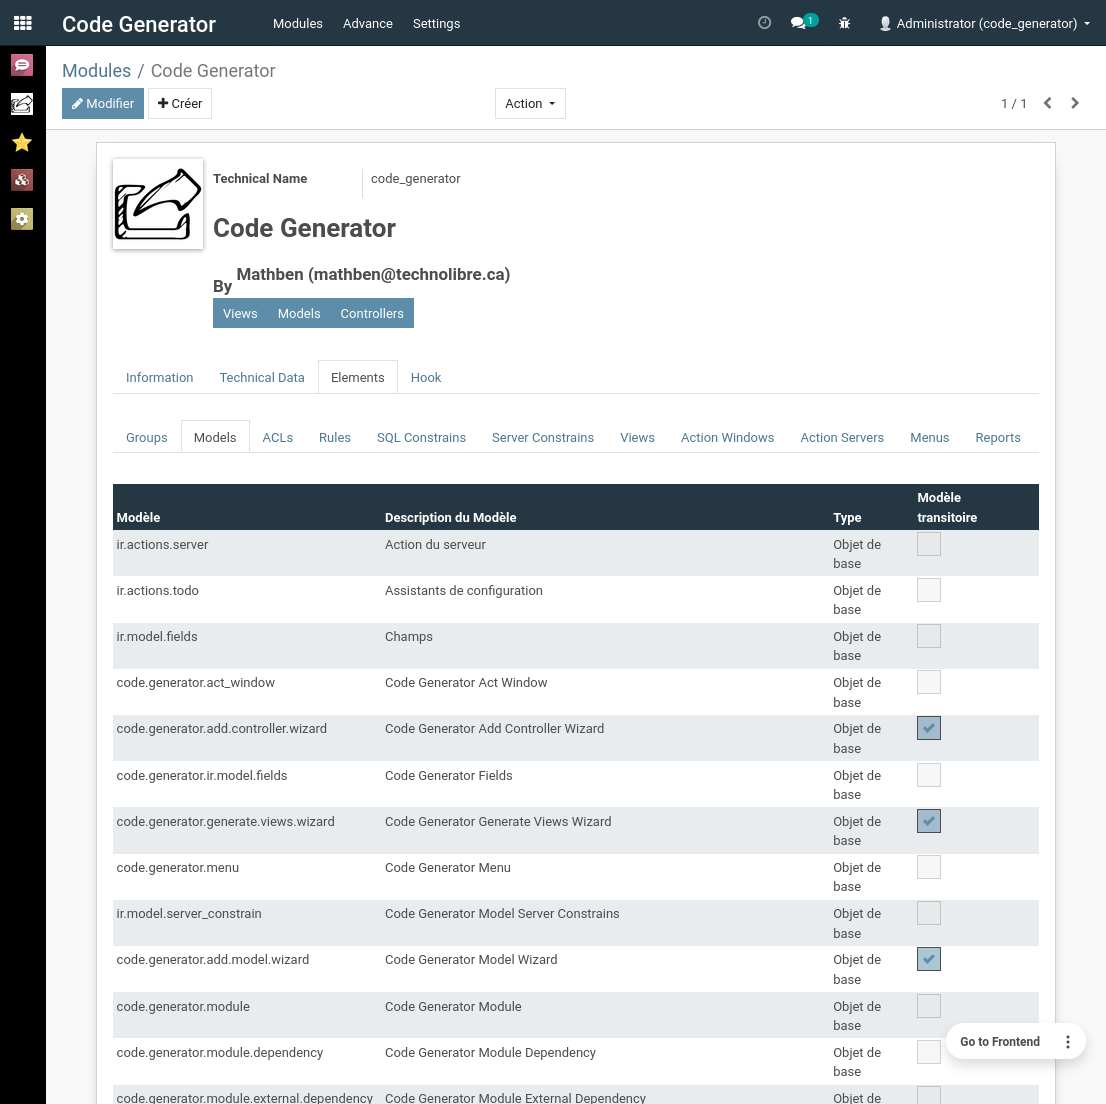
\includegraphics[width=6.535in]{cg_model.png}
\end{figure}

\Annexe{GUI générateur de code - les champs} \label{annexe_cg_gui_champs}

\begin{figure}[htb]
\centering
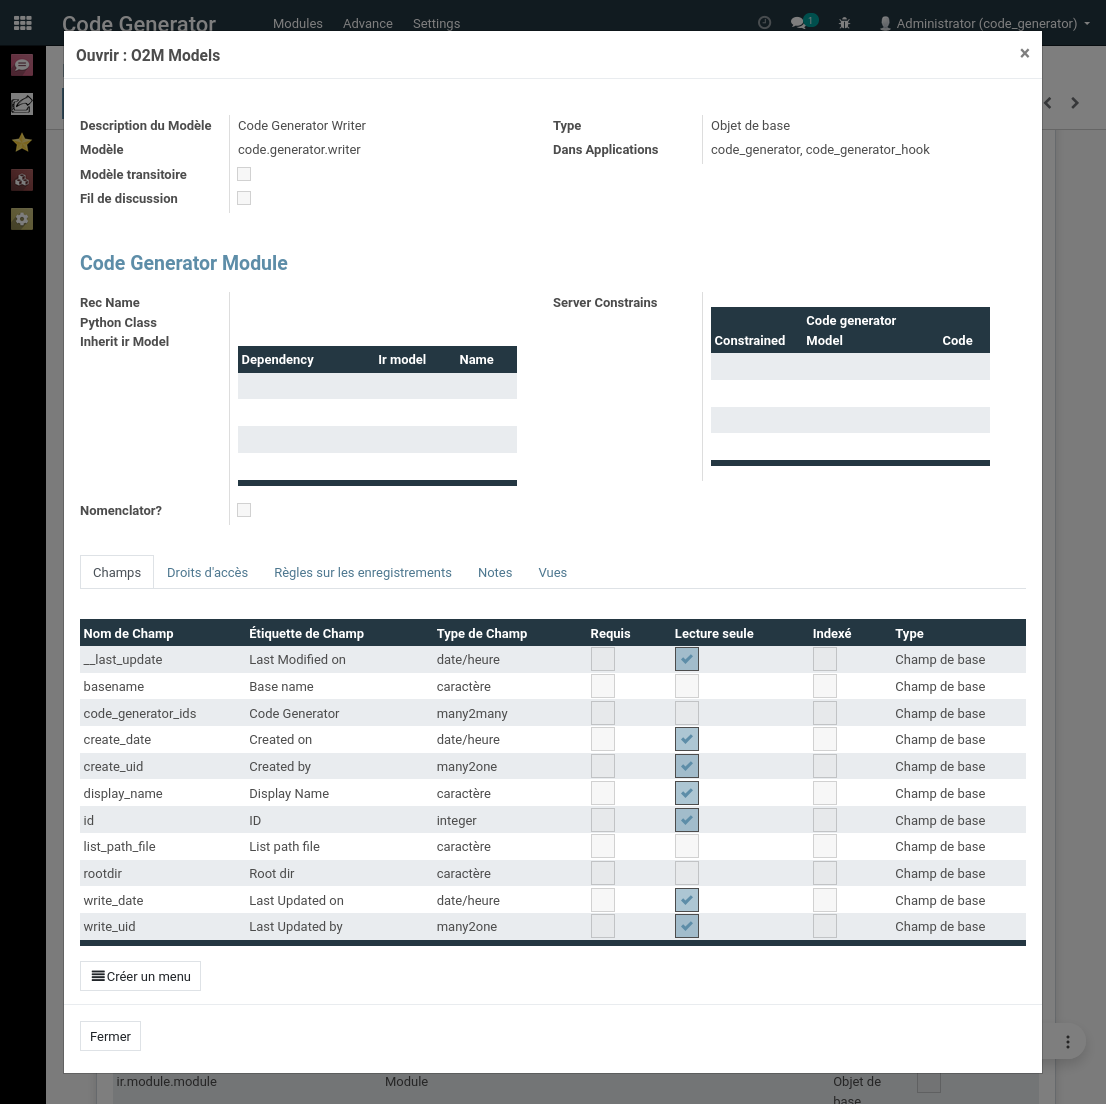
\includegraphics[width=6.535in]{cg_champs.png}
\end{figure}

\Annexe{GUI générateur de code - les codes} \label{annexe_cg_gui_code}

\begin{figure}[htb]
\centering
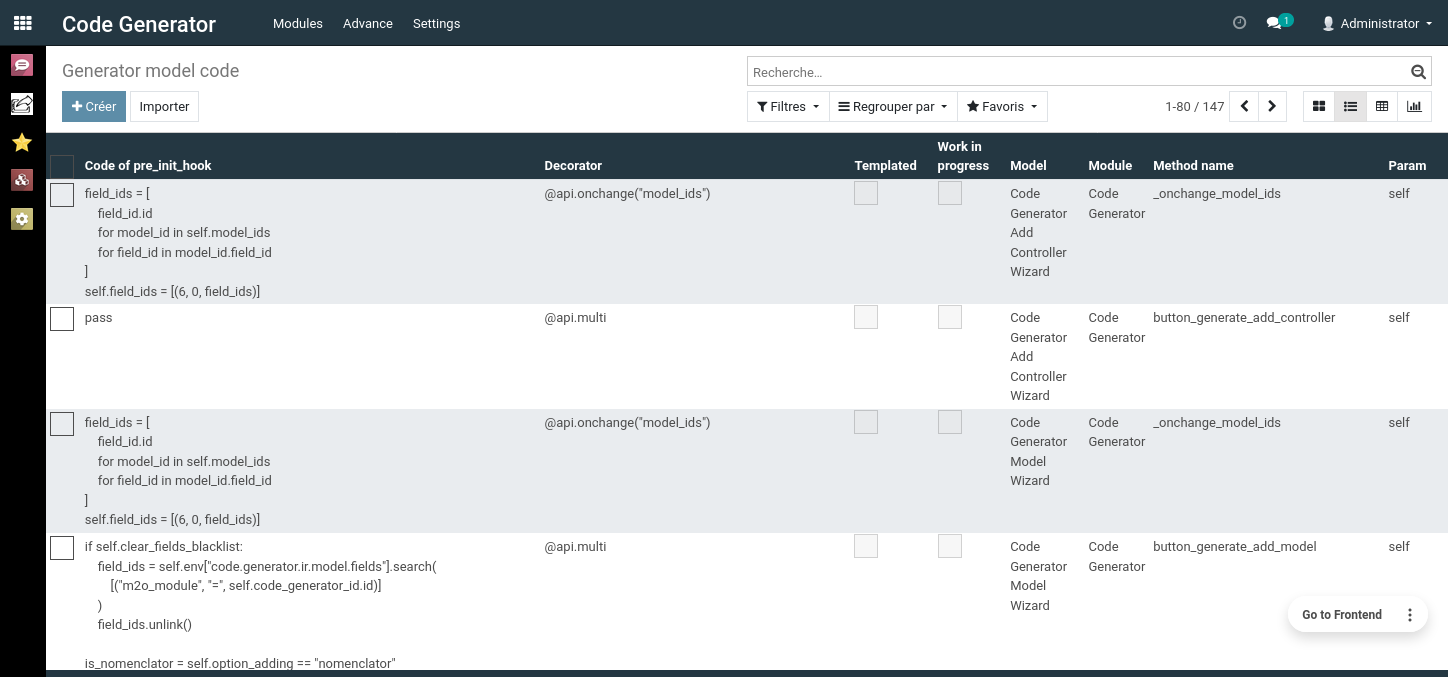
\includegraphics[width=6.535in]{cg_code.png}
\end{figure}

\Annexe{GUI générateur de code - les «hooks»} \label{annexe_cg_gui_hook}

\begin{figure}[htb]
\centering
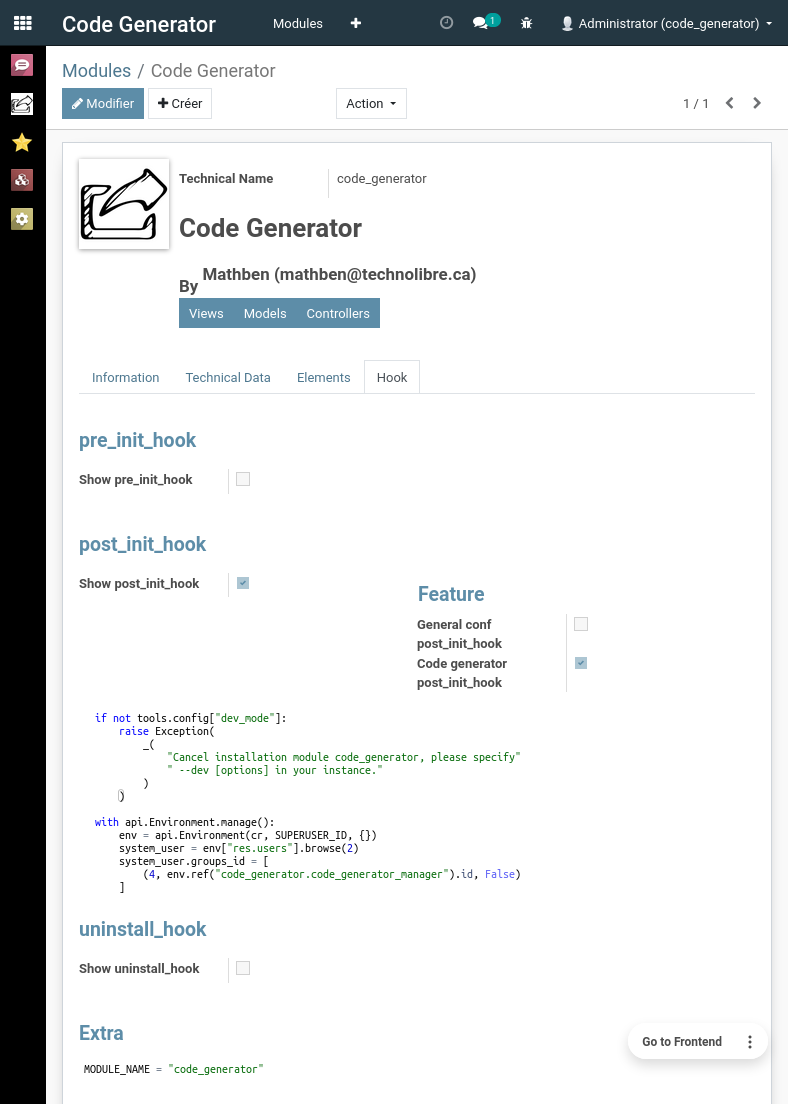
\includegraphics[height=7in]{cg_hook.png}
\end{figure}


\Annexe{Test couverture technique générateur de code} \label{annexe_test_generateur_code}

\begin{table}[htb]
\centering
\begin{tabular}{|l|l|l|l|l|l|}

\hline
\cellcolor[HTML]{d9d9d9}{\textbf{Technique}} & \multicolumn{2}{|l|}{\cellcolor[HTML]{d9d9d9}{base}} & \multicolumn{2}{|l|}{\cellcolor[HTML]{d9d9d9}{\textbf{\# instruction}}} & \cellcolor[HTML]{d9d9d9}{5 085}\\\hline

\multicolumn{2}{|l|}{\cellcolor[HTML]{efefef}{\textbf{Description du test}}} & \cellcolor[HTML]{efefef}{\textbf{Status}} & \cellcolor[HTML]{efefef}{\textbf{Durée (s)}} & \cellcolor[HTML]{efefef}{\textbf{\# de Miss}} & \cellcolor[HTML]{efefef}{\textbf{Cover (\%)}}\\\hline

\multicolumn{2}{|l|}{\shortstack[l]{Génération µ$_C^B$ modèle simple}} & Succès & 27 & 2 983 & 41\\\hline

\multicolumn{2}{|l|}{\shortstack[l]{Génération µ$_C^B$ modèle simple avec \\ héritage}} & Succès & 26 & 3 452 & 32\\\hline

\multicolumn{2}{|l|}{\shortstack[l]{Exportation µ$_C^B$ données «helpdesk»}} & Succès & 28 & 3 900 & 23\\\hline

% \end{tabular}
% \end{table}
% \begin{table}
% \centering
% \begin{tabular}{|l|l|l|l|l|l|}
% \hline

\cellcolor[HTML]{d9d9d9}{\textbf{Technique}} & \multicolumn{2}{|l|}{\cellcolor[HTML]{d9d9d9}{base + hook}} & \multicolumn{2}{|l|}{\cellcolor[HTML]{d9d9d9}{\textbf{\# instruction}}} & \cellcolor[HTML]{d9d9d9}{5 985}\\\hline

\multicolumn{2}{|l|}{\cellcolor[HTML]{efefef}{\textbf{Description du test}}} & \cellcolor[HTML]{efefef}{\textbf{Status}} & \cellcolor[HTML]{efefef}{\textbf{Durée (s)}} & \cellcolor[HTML]{efefef}{\textbf{\# de Miss}} & \cellcolor[HTML]{efefef}{\textbf{Cover (\%)}}\\\hline

\multicolumn{2}{|l|}{\shortstack[l]{Auto-génération µ$_C^0$}} & Succès & 17 & 4 683 & 22\\\hline

\multicolumn{2}{|l|}{\shortstack[l]{Nouveau projet µ$_C^0$ µ$_C^A$ µ$_C^B$ \\ «Hello World»}} & Succès & 39 & 4 610 & 23\\\hline

\multicolumn{2}{|l|}{\shortstack[l]{Génération µ$_C^A$ portail}} & Succès & 44 & 3 638 & 39\\\hline

\multicolumn{2}{|l|}{\shortstack[l]{Génération µ$_C^A$ modèle simple}} & Succès & 33 & 3 982 & 33\\\hline

\multicolumn{2}{|l|}{\shortstack[l]{Génération µ$_C^A$ modèle simple avec \\ héritage}} & Succès & 32 & 4 027 & 33\\\hline

\multicolumn{2}{|l|}{\shortstack[l]{Exportation µ$_C^B$ données «website»}} & Succès & 28 & 3 900 & 23\\\hline

\multicolumn{2}{|l|}{\shortstack[l]{Génération µ$_C^B$ du générateur de \\ code}} & Échec & 20 & 3 529 & 41\\\hline

\multicolumn{2}{|l|}{\shortstack[l]{Génération µ$_C^A$ du générateur de \\ code}} & Échec & 29 & 3 690 & 38\\\hline

% \end{tabular}
% \end{table}
% \begin{table}
% \centering
% \begin{tabular}{|l|l|l|l|l|l|}
% \hline

\cellcolor[HTML]{d9d9d9}{\textbf{Technique}} & \multicolumn{2}{|l|}{\cellcolor[HTML]{d9d9d9}{base + cron}} & \multicolumn{2}{|l|}{\cellcolor[HTML]{d9d9d9}{\textbf{\# instruction}}} & \cellcolor[HTML]{d9d9d9}{6 153}\\\hline

\multicolumn{2}{|l|}{\cellcolor[HTML]{efefef}{\textbf{Description du test}}} & \cellcolor[HTML]{efefef}{\textbf{Status}} & \cellcolor[HTML]{efefef}{\textbf{Durée (s)}} & \cellcolor[HTML]{efefef}{\textbf{\# de Miss}} & \cellcolor[HTML]{efefef}{\textbf{Cover (\%)}}\\\hline

\multicolumn{2}{|l|}{\shortstack[l]{Génération µ$_C^A$ «auto\_backup»}} & Succès & 36 & 3 422 & 44\\\hline

% \end{tabular}
% \end{table}
% \begin{table}
% \centering
% \begin{tabular}{|l|l|l|l|l|l|}
% \hline

\cellcolor[HTML]{d9d9d9}{\textbf{Technique}} & \multicolumn{2}{|l|}{\cellcolor[HTML]{d9d9d9}{base + portal}} & \multicolumn{2}{|l|}{\cellcolor[HTML]{d9d9d9}{\textbf{\# instruction}}} & \cellcolor[HTML]{d9d9d9}{5 799}\\\hline

\multicolumn{2}{|l|}{\cellcolor[HTML]{efefef}{\textbf{Description du test}}} & \cellcolor[HTML]{efefef}{\textbf{Status}} & \cellcolor[HTML]{efefef}{\textbf{Durée (s)}} & \cellcolor[HTML]{efefef}{\textbf{\# de Miss}} & \cellcolor[HTML]{efefef}{\textbf{Cover (\%)}}\\\hline

\multicolumn{2}{|l|}{\shortstack[l]{Génération µ$_C^B$ exemple MariaDB \\ \texttt{SQL}}} & Succès & 80 & 3 104 & 46\\\hline

% \end{tabular}
% \end{table}
% \begin{table}
% \centering
% \begin{tabular}{|l|l|l|l|l|l|}
% \hline

\cellcolor[HTML]{d9d9d9}{\textbf{Technique}} & \multicolumn{2}{|l|}{\cellcolor[HTML]{d9d9d9}{base + «theme\_website»}} & \multicolumn{2}{|l|}{\cellcolor[HTML]{d9d9d9}{\textbf{\# instruction}}} & \cellcolor[HTML]{d9d9d9}{5 336}\\\hline

\multicolumn{2}{|l|}{\cellcolor[HTML]{efefef}{\textbf{Description du test}}} & \cellcolor[HTML]{efefef}{\textbf{Status}} & \cellcolor[HTML]{efefef}{\textbf{Durée (s)}} & \cellcolor[HTML]{efefef}{\textbf{\# de Miss}} & \cellcolor[HTML]{efefef}{\textbf{Cover (\%)}}\\\hline

\multicolumn{2}{|l|}{\shortstack[l]{Génération µ$_C^B$ thème «website»}} & Succès & 27 & 3 938 & 26\\\hline

% \end{tabular}
% \end{table}
% \begin{table}
% \centering
% \begin{tabular}{|l|l|l|l|l|l|}
% \hline

\cellcolor[HTML]{d9d9d9}{\textbf{Technique}} & \multicolumn{2}{|l|}{\cellcolor[HTML]{d9d9d9}{base + «website\_snippet»}} & \multicolumn{2}{|l|}{\cellcolor[HTML]{d9d9d9}{\textbf{\# instruction}}} & \cellcolor[HTML]{d9d9d9}{5 615}\\\hline

\multicolumn{2}{|l|}{\cellcolor[HTML]{efefef}{\textbf{Description du test}}} & \cellcolor[HTML]{efefef}{\textbf{Status}} & \cellcolor[HTML]{efefef}{\textbf{Durée (s)}} & \cellcolor[HTML]{efefef}{\textbf{\# de Miss}} & \cellcolor[HTML]{efefef}{\textbf{Cover (\%)}}\\\hline

\multicolumn{2}{|l|}{\shortstack[l]{Génération µ$_C^B$ individuel \\ «website\_snippet»}} & Succès & 26 & 4 284 & 24\\\hline

\end{tabular}
\end{table}
\begin{table}[htb]
\centering
\begin{tabular}{|l|l|l|l|l|l|}
\hline

\cellcolor[HTML]{d9d9d9}{\textbf{Technique}} & \multicolumn{2}{|l|}{\cellcolor[HTML]{d9d9d9}{\shortstack[l]{base + portal + \\ «website\_snippet»}}} & \multicolumn{2}{|l|}{\cellcolor[HTML]{d9d9d9}{\textbf{\# instruction}}} & \cellcolor[HTML]{d9d9d9}{6 329}\\\hline

\multicolumn{2}{|l|}{\cellcolor[HTML]{efefef}{\textbf{Description du test}}} & \cellcolor[HTML]{efefef}{\textbf{Status}} & \cellcolor[HTML]{efefef}{\textbf{Durée (s)}} & \cellcolor[HTML]{efefef}{\textbf{\# de Miss}} & \cellcolor[HTML]{efefef}{\textbf{Cover (\%)}}\\\hline

\multicolumn{2}{|l|}{\shortstack[l]{Génération µ$_C^B$ multiple \\ «website\_snippet»}} & Succès & 36 & 2 898 & 54\\\hline

\multicolumn{2}{|l|}{\shortstack[l]{Génération µ$_C^B$ portail}} & Succès & 34 & 3 173 & 50\\\hline

% \end{tabular}
% \end{table}
% \begin{table}
% \centering
% \begin{tabular}{|l|l|l|l|l|l|}
% \hline

\cellcolor[HTML]{d9d9d9}{\textbf{Technique}} & \multicolumn{2}{|l|}{\cellcolor[HTML]{d9d9d9}{base + portal + «Migration DB»}} & \multicolumn{2}{|l|}{\cellcolor[HTML]{d9d9d9}{\textbf{\# instruction}}} & \cellcolor[HTML]{d9d9d9}{6 559}\\\hline

\multicolumn{2}{|l|}{\cellcolor[HTML]{efefef}{\textbf{Description du test}}} & \cellcolor[HTML]{efefef}{\textbf{Status}} & \cellcolor[HTML]{efefef}{\textbf{Durée (s)}} & \cellcolor[HTML]{efefef}{\textbf{\# de Miss}} & \cellcolor[HTML]{efefef}{\textbf{Cover (\%)}}\\\hline

\multicolumn{2}{|l|}{\shortstack[l]{Génération migration MariaDB \\ \texttt{SQL}}} & Succès & 121 & 3 267 & 50\\\hline

% \end{tabular}
% \end{table}
% \begin{table}
% \centering
% \begin{tabular}{|l|l|l|l|l|l|}

\hline
\cellcolor[HTML]{d9d9d9}{\textbf{Technique}} & \multicolumn{2}{|l|}{\cellcolor[HTML]{d9d9d9}{base + hook + portal}} & \multicolumn{2}{|l|}{\cellcolor[HTML]{d9d9d9}{\textbf{\# instruction}}} & \cellcolor[HTML]{d9d9d9}{6 699}\\\hline

\multicolumn{2}{|l|}{\cellcolor[HTML]{efefef}{\textbf{Description du test}}} & \cellcolor[HTML]{efefef}{\textbf{Status}} & \cellcolor[HTML]{efefef}{\textbf{Durée (s)}} & \cellcolor[HTML]{efefef}{\textbf{\# de Miss}} & \cellcolor[HTML]{efefef}{\textbf{Cover (\%)}}\\\hline

\multicolumn{2}{|l|}{\shortstack[l]{Génération µ$_C^A$ MariaDB \texttt{SQL}}} & Succès & 78 & 4 315 & 36\\\hline

% \end{tabular}
% \end{table}
% \begin{table}
% \centering
% \begin{tabular}{|l|l|l|l|l|l|}
% \hline

\cellcolor[HTML]{d9d9d9}{\textbf{Technique}} & \multicolumn{2}{|l|}{\cellcolor[HTML]{d9d9d9}{base + hook + cron}} & \multicolumn{2}{|l|}{\cellcolor[HTML]{d9d9d9}{\textbf{\# instruction}}} & \cellcolor[HTML]{d9d9d9}{6 153}\\\hline

\multicolumn{2}{|l|}{\cellcolor[HTML]{efefef}{\textbf{Description du test}}} & \cellcolor[HTML]{efefef}{\textbf{Status}} & \cellcolor[HTML]{efefef}{\textbf{Durée (s)}} & \cellcolor[HTML]{efefef}{\textbf{\# de Miss}} & \cellcolor[HTML]{efefef}{\textbf{Cover (\%)}}\\\hline

\multicolumn{2}{|l|}{\shortstack[l]{Génération µ$_C^A$ «auto\_backup»}} & Succès & 36 & 3 422 & 44\\\hline

% \end{tabular}
% \end{table}
% \begin{table}
% \centering
% \begin{tabular}{|l|l|l|l|l|l|}
% \hline

\cellcolor[HTML]{d9d9d9}{\textbf{Technique}} & \multicolumn{2}{|l|}{\cellcolor[HTML]{d9d9d9}{\shortstack[l]{base + geoengine + \\ «website\_leaflet»}}} & \multicolumn{2}{|l|}{\cellcolor[HTML]{d9d9d9}{\textbf{\# instruction}}} & \cellcolor[HTML]{d9d9d9}{5 423}\\\hline

\multicolumn{2}{|l|}{\cellcolor[HTML]{efefef}{\textbf{Description du test}}} & \cellcolor[HTML]{efefef}{\textbf{Status}} & \cellcolor[HTML]{efefef}{\textbf{Durée (s)}} & \cellcolor[HTML]{efefef}{\textbf{\# de Miss}} & \cellcolor[HTML]{efefef}{\textbf{Cover (\%)}}\\\hline

\multicolumn{2}{|l|}{\shortstack[l]{Génération µ$_C^B$ \\ «website\_snippet\_leaflet»}} & Succès & 33 & 3 259 & 40\\\hline

% \end{tabular}
% \end{table}
% \begin{table}
% \centering
% \begin{tabular}{|l|l|l|l|l|l|}
% \hline

\cellcolor[HTML]{d9d9d9}{\textbf{Technique}} & \multicolumn{2}{|l|}{\cellcolor[HTML]{d9d9d9}{\shortstack[l]{base + cron + hook + \\ «Migration DB» + geoengine + \\ portal + «theme\_website» + \\ «website\_snippet» + \\ «website\_leaflet»}}} & \multicolumn{2}{|l|}{\cellcolor[HTML]{d9d9d9}{\textbf{\# instruction}}} & \cellcolor[HTML]{d9d9d9}{8 746}\\\hline

\multicolumn{2}{|l|}{\cellcolor[HTML]{efefef}{\textbf{Description du test}}} & \cellcolor[HTML]{efefef}{\textbf{Status}} & \cellcolor[HTML]{efefef}{\textbf{Durée (s)}} & \cellcolor[HTML]{efefef}{\textbf{\# de Miss}} & \cellcolor[HTML]{efefef}{\textbf{Cover (\%)}}\\\hline

\multicolumn{2}{|l|}{\shortstack[l]{Tous les tests à succès}} & Succès & 194 & 1 371 & 84\\\hline

\end{tabular}
\end{table}

\Annexe{Diagramme modèle de données Espace Membre Accorderie 2019} \label{annexe_db_accorderie_2019}

\begin{figure}[htb]
\centering
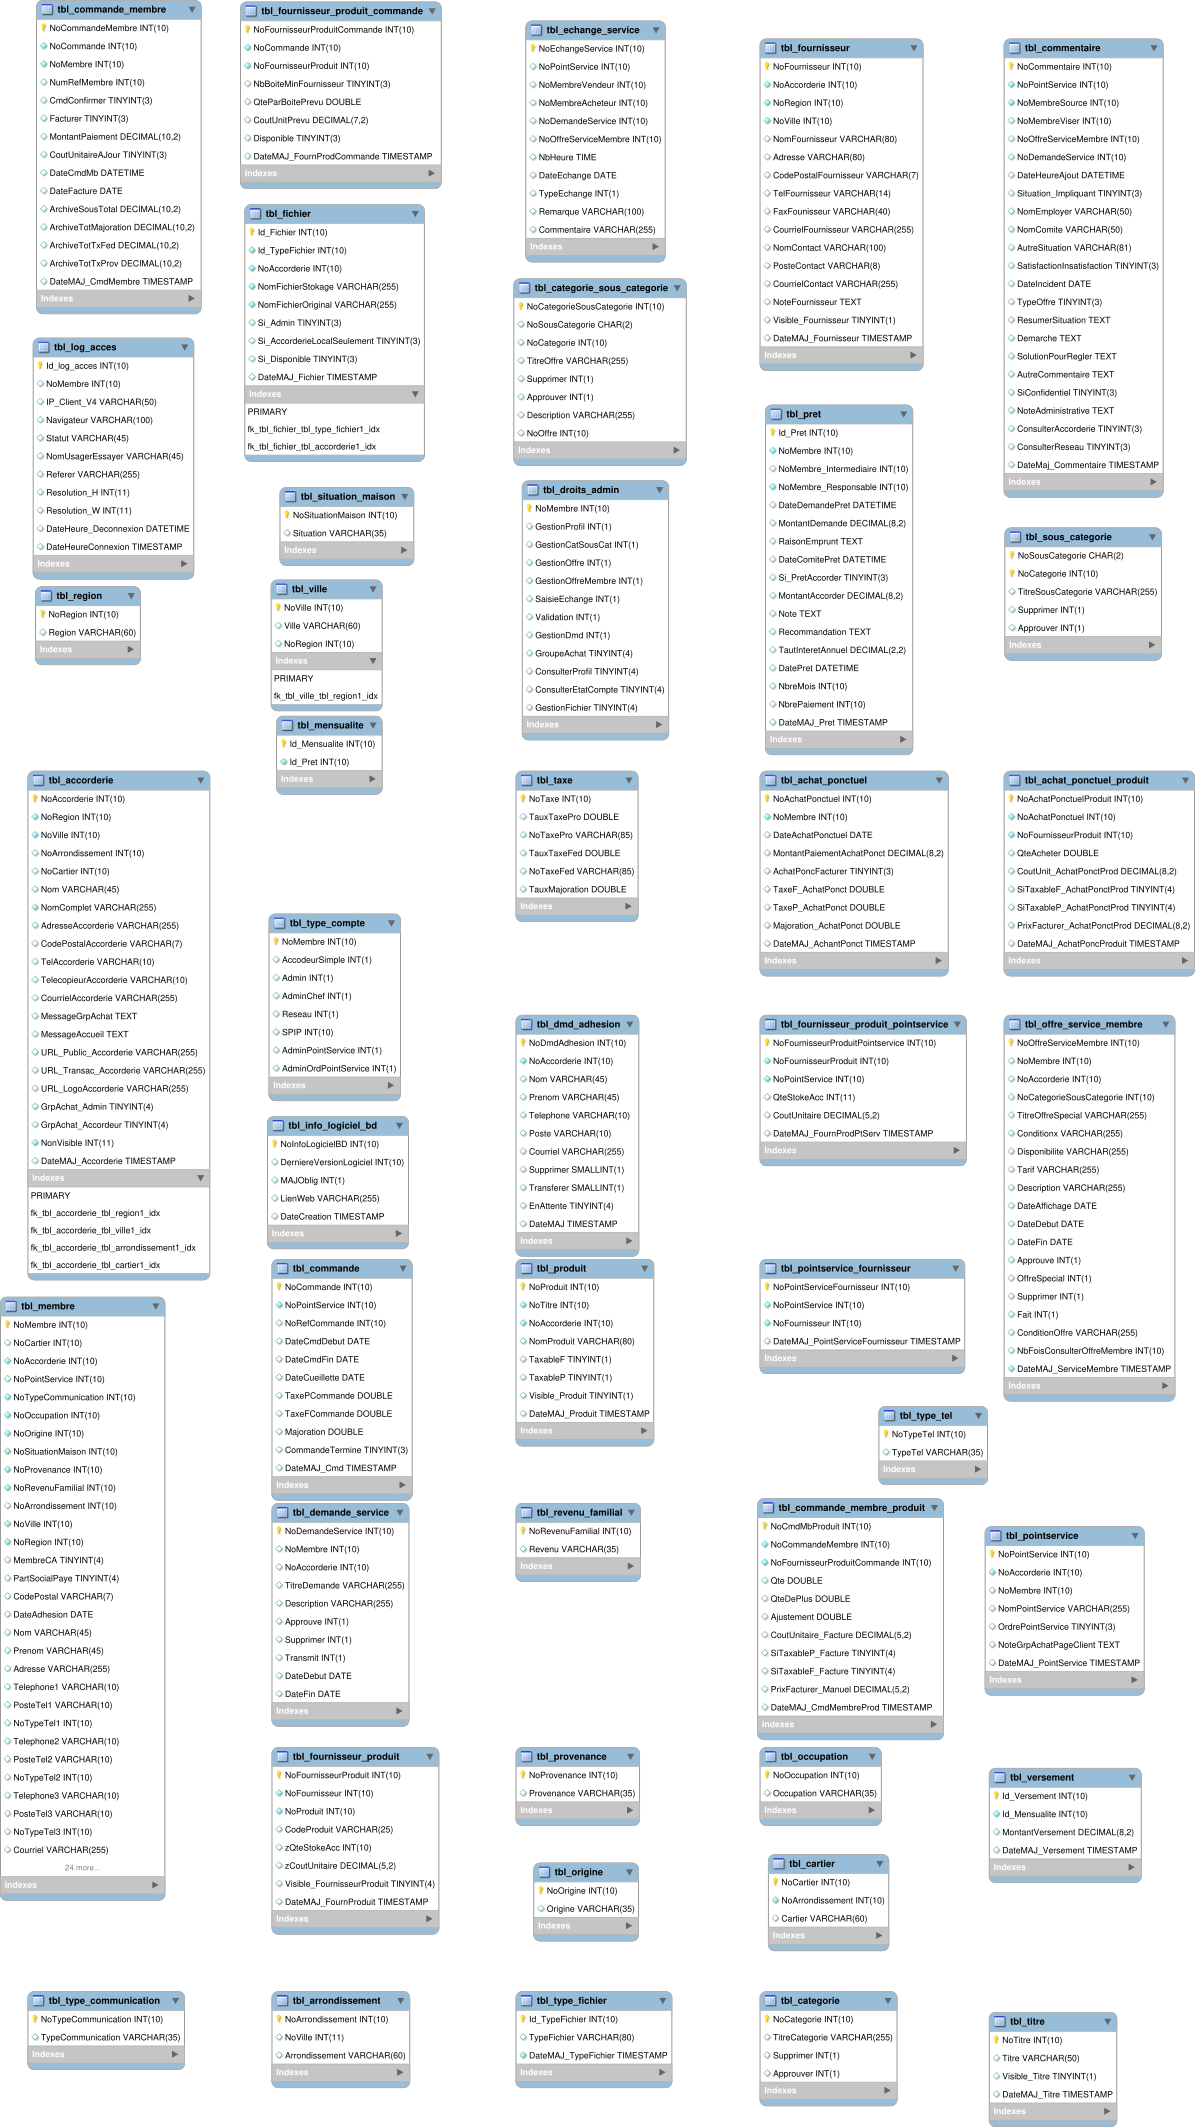
\includegraphics[height=7in]{schema_bd_accorderie.png}
\end{figure}

\Annexe{Diagramme nouveau modèle de données Espace Membre Accorderie 2023} \label{annexe_db_accorderie_2023}

\begin{figure}[htb]
\centering
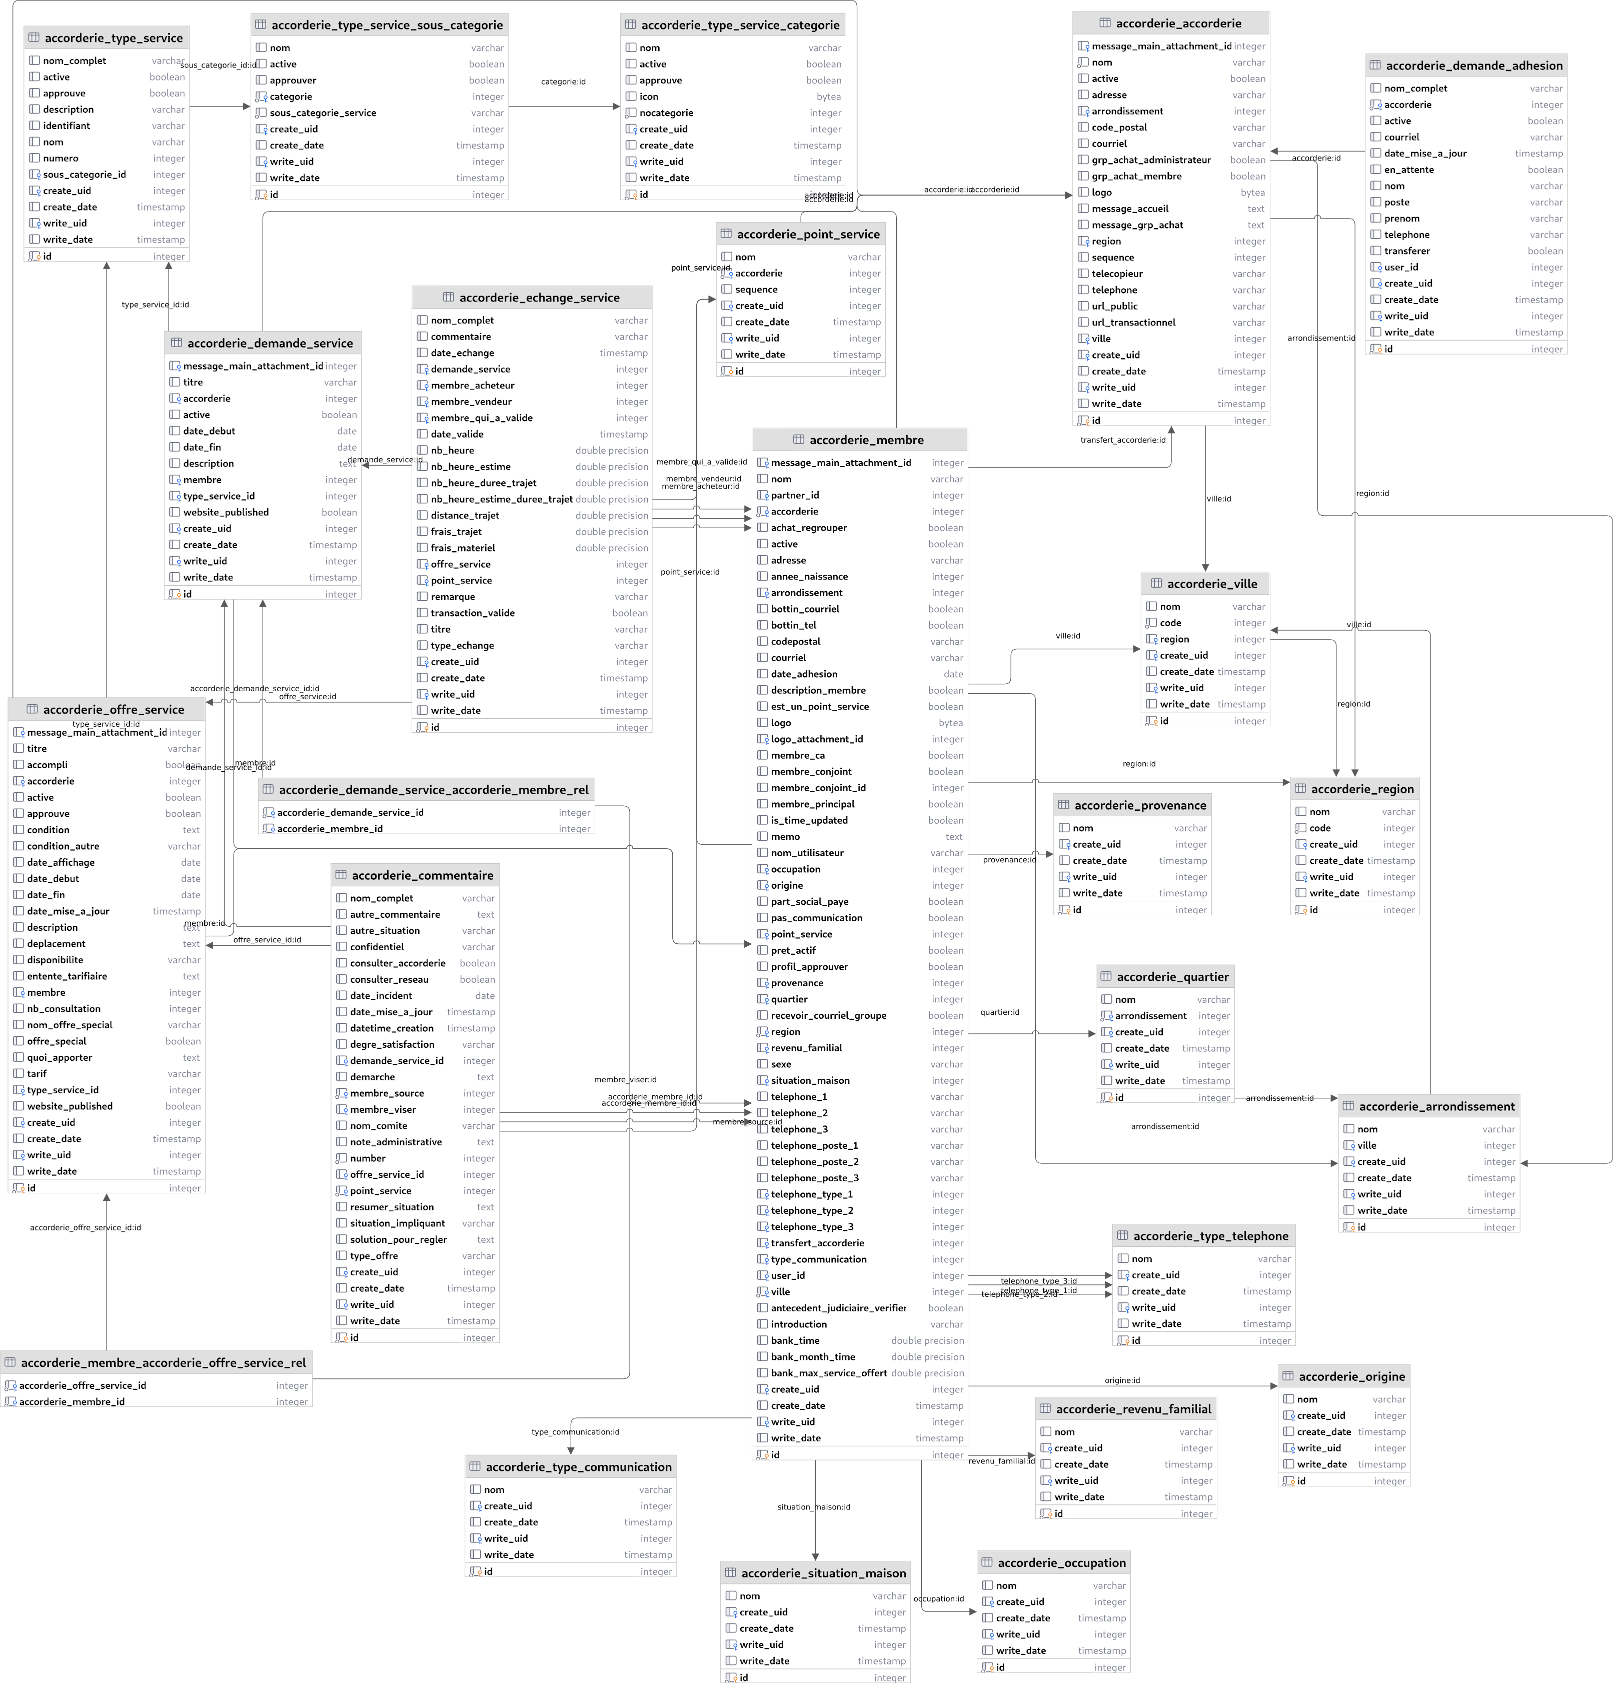
\includegraphics[width=6.535in]{schema_bd_accorderie_new_small.png}
\end{figure}

\Annexe{Diagramme processus pour demander, offrir, établir un échange et le valider - Accorderie 2023} \label{annexe_processus_accorderie_2023}

\begin{figure}[htb]
\centering
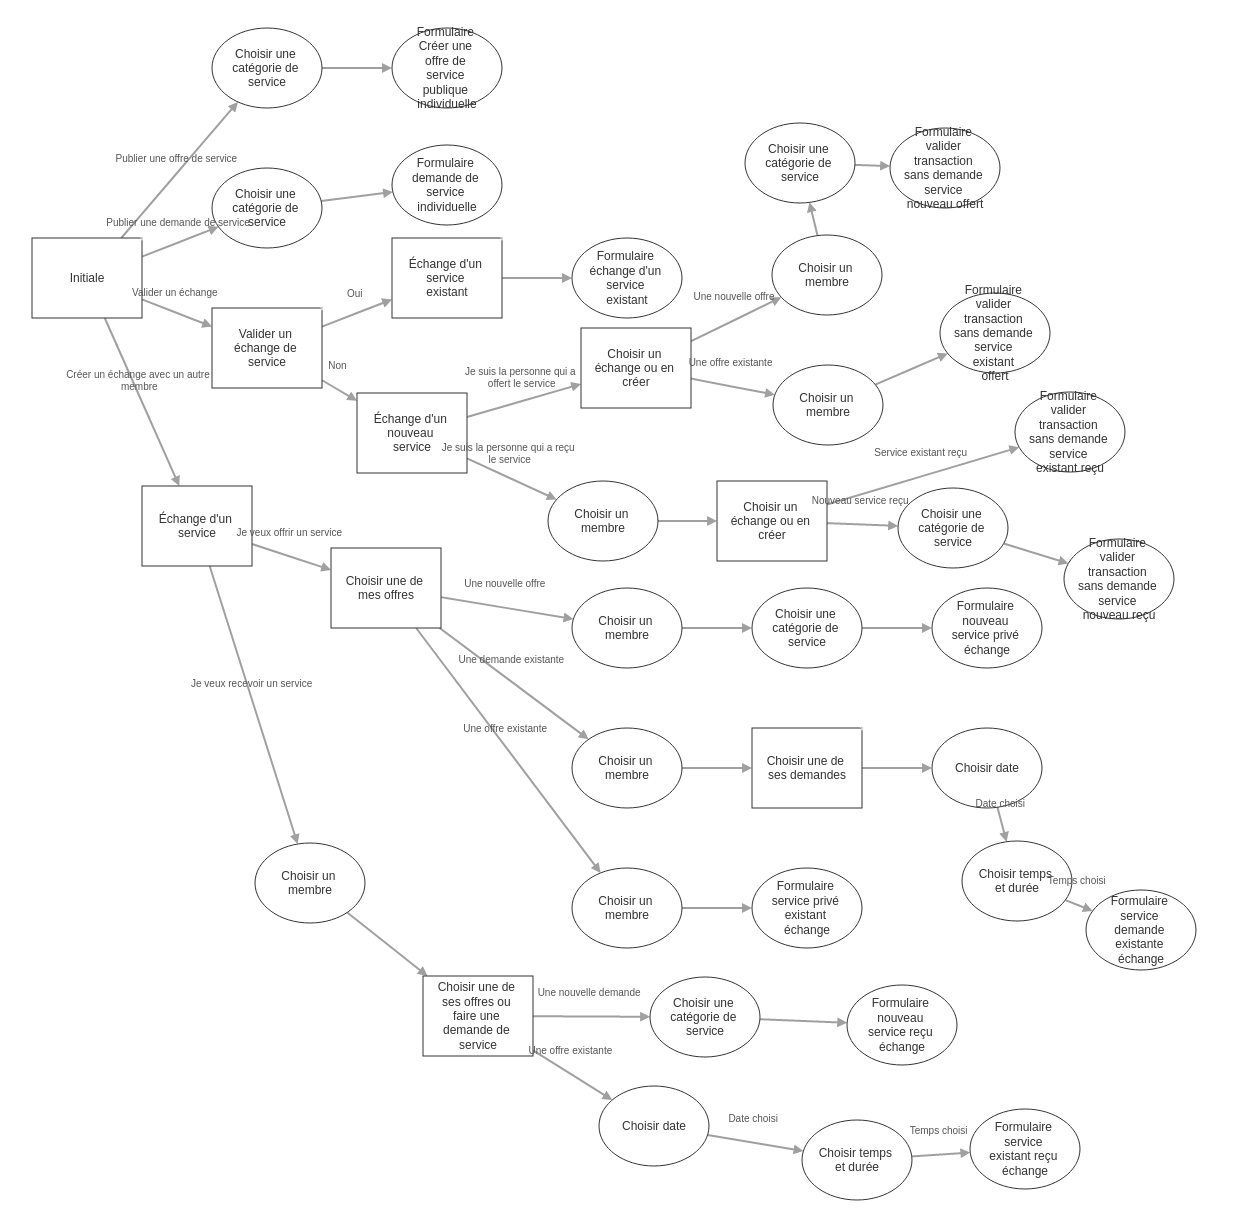
\includegraphics[width=6.535in]{accorderie_processus.png}
\end{figure}

\Annexe{Diagramme modèle de données du portail CEPPP septembre 2022} \label{annexe_db_ceppp_2022}

\begin{figure}[htb]
\centering
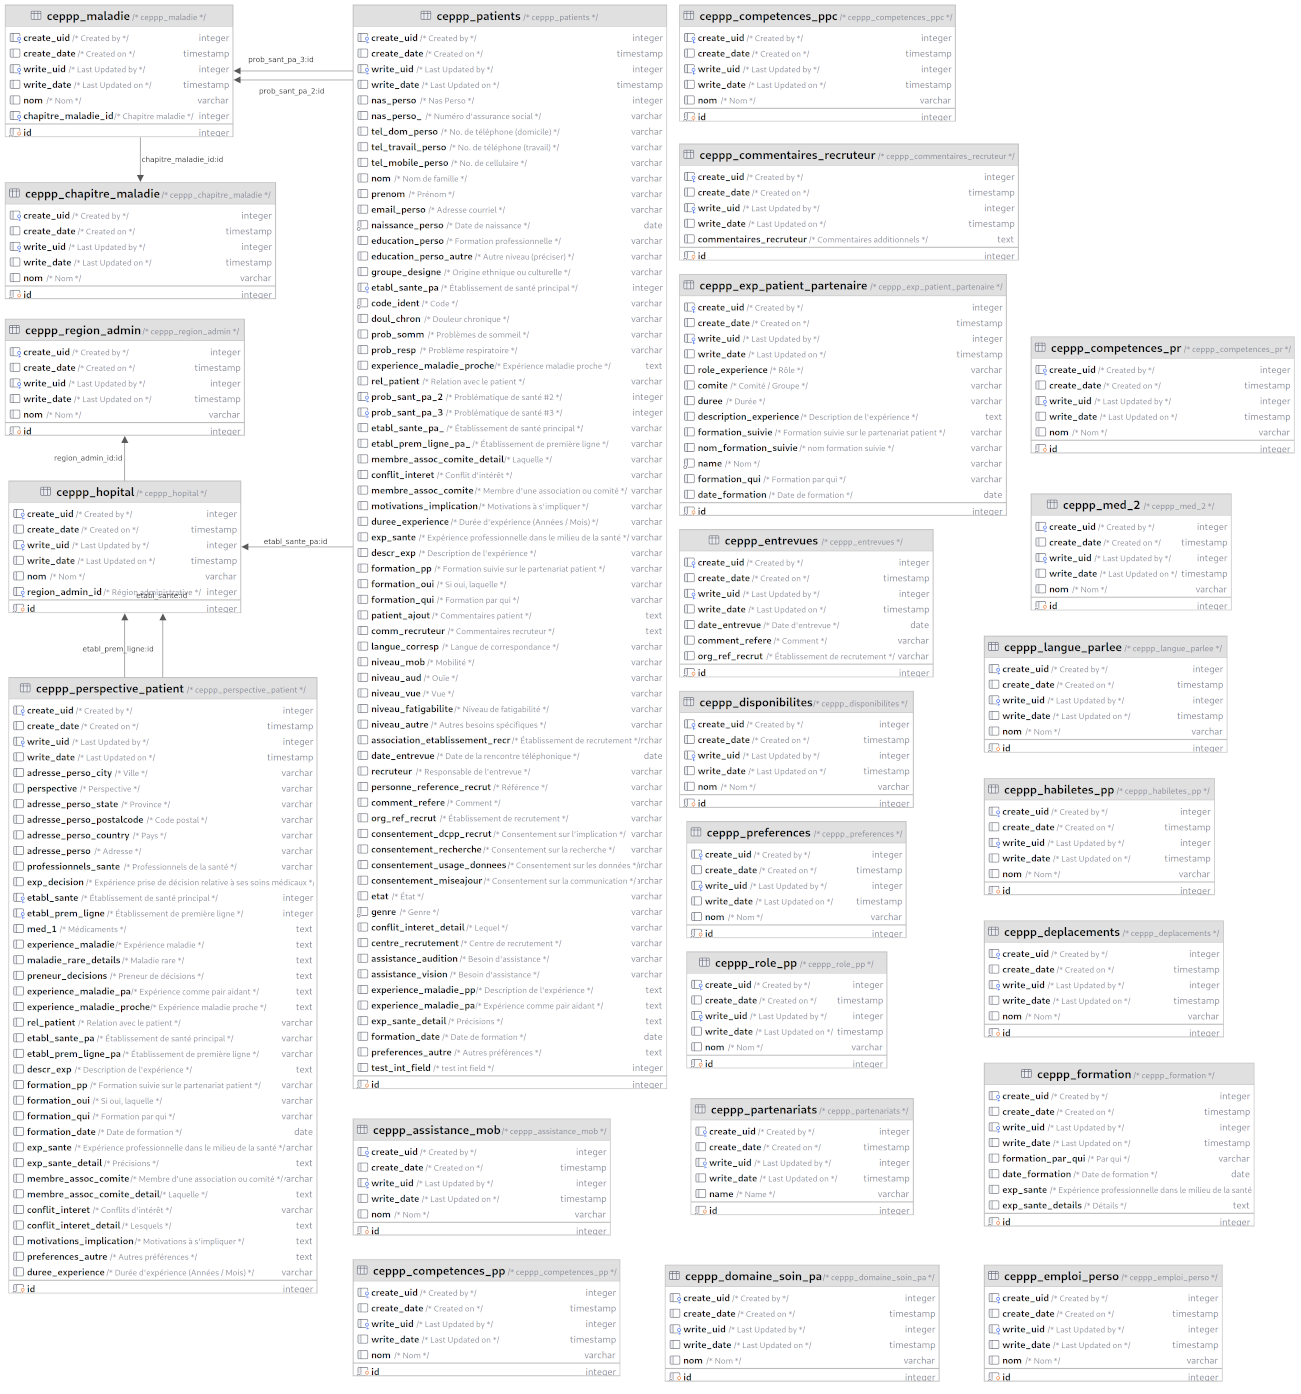
\includegraphics[width=6.535in]{schema_bd_ceppp_suite_crm_small.png}
\end{figure}

\Annexe{Vue formulaire administration portail CEPPP} \label{annexe_form_ceppp_2022}

\begin{figure}[htb]
\centering
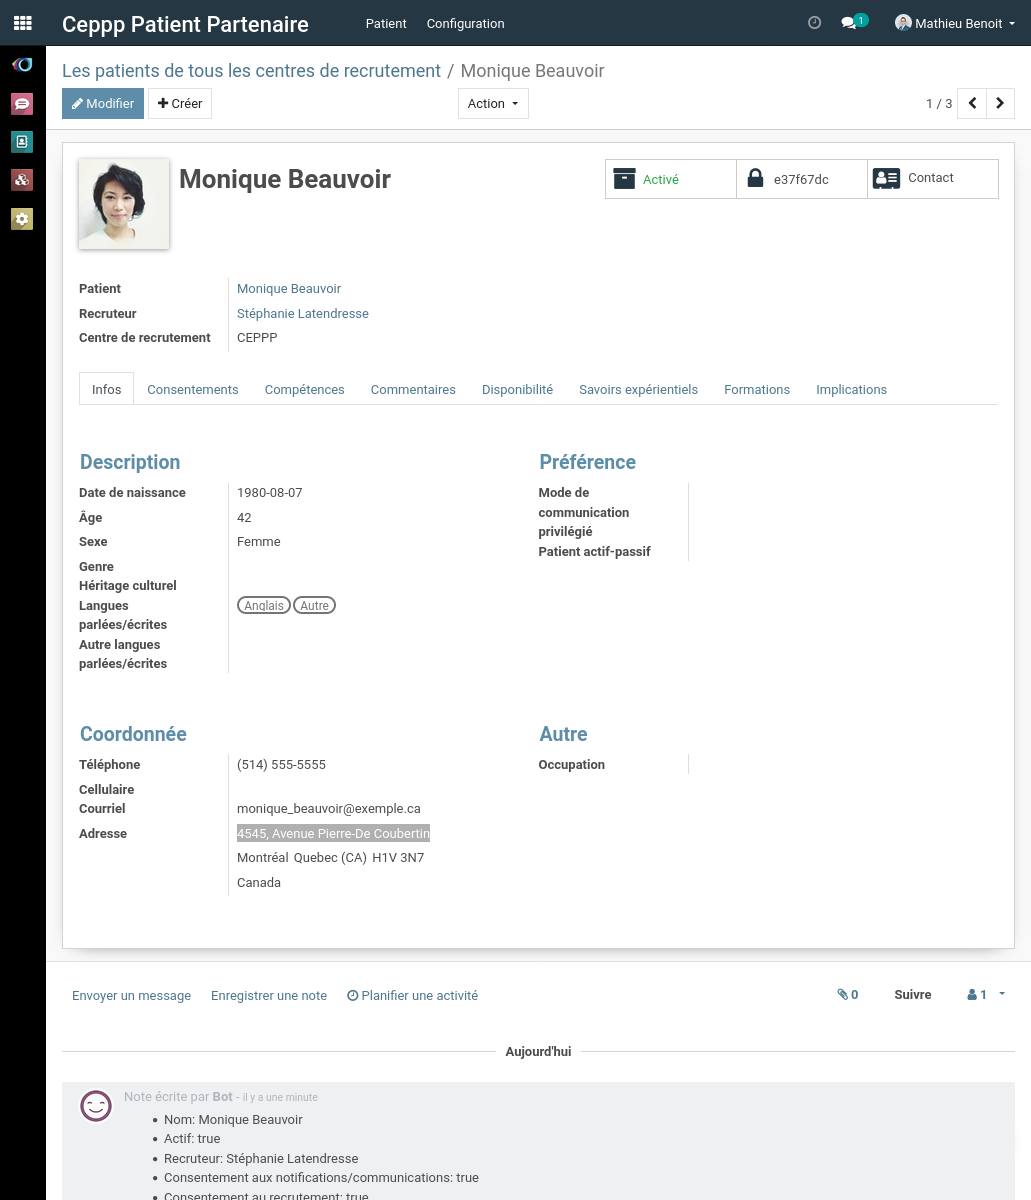
\includegraphics[height=7in]{exemple_vue_formulaire_patient_ceppp.png}
\end{figure}

\Annexe{Vue formulaire partenaire portail CEPPP} \label{annexe_form_anonyme_ceppp_2022}

\begin{figure}[htb]
\centering
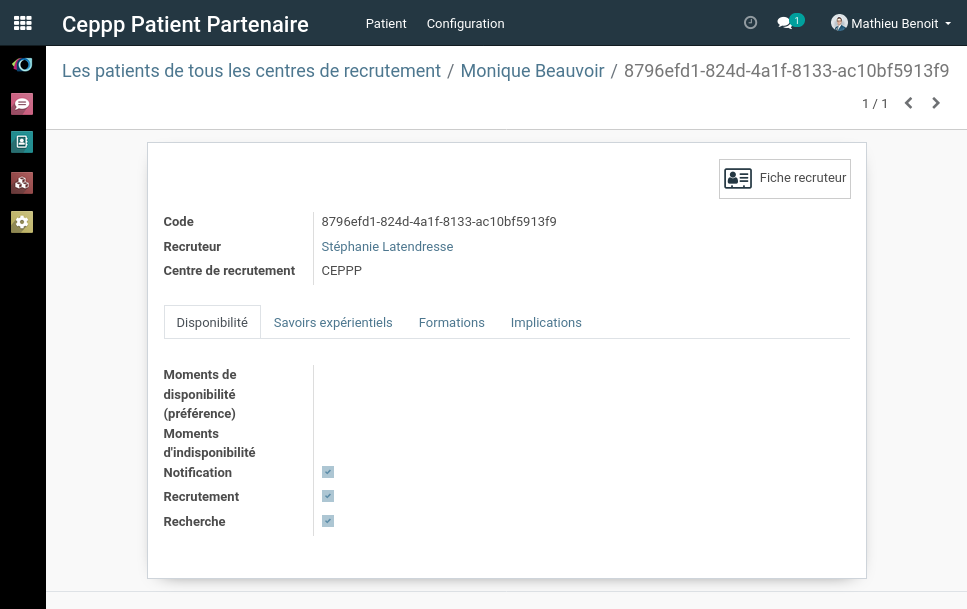
\includegraphics[width=6.535in]{exemple_vue_formulaire_patient_anonyme_ceppp.png}
\end{figure}
}
{}
\end{document}
